\documentclass[11pt]{article}
\renewcommand{\cite}[2][]{%
\ifx&#2&
    \parentcite{#1}%
\else
    \parencite[#1]{#2}%
\fi
}

\usepackage[utf8]{inputenc}
\usepackage[T1]{fontenc}
\usepackage{lmodern}
\usepackage[left=2.5cm, right=2.5cm, top=2.5cm,  bottom=2.5cm]{geometry}
\usepackage[activate]{microtype}
\usepackage[american]{babel}
\usepackage{verbatim}
\usepackage{graphicx}
\usepackage{svg}
\usepackage{xcolor}
\usepackage{csquotes}
\usepackage{amsmath}
\usepackage{amssymb}
\usepackage{nth}
\usepackage{listings}
\usepackage{wrapfig}
\usepackage{float}
\usepackage[inline]{enumitem}
\setlist{noitemsep}
\renewcommand{\labelitemi}{$-$}

\usepackage{placeins}
\usepackage{footnote}



\usepackage[
	pdftitle={},
	pdfauthor={},
	pdfcreator={pdflatex, LaTeX with KOMA-Script},
	pdfpagemode=UseOutlines,
	pdfdisplaydoctitle=true,
	pdflang={english}
]{hyperref}

\hypersetup{
	colorlinks=true,
	linkcolor=black,
	citecolor=black,
	filecolor=black,
	menucolor=black,
	urlcolor=black,
	linktocpage=true,
	bookmarksnumbered=true,
	linktoc=all
}

\usepackage[
	backend=biber,
	bibwarn=true,
	bibencoding=utf8,
	sortlocale=en_US,
	style=numeric
]{biblatex}

\bibliography{bibliography} 

\DeclareLanguageMapping{american}{american-apa}

\renewcommand{\cite}{\parencite}
\usepackage{cleveref}

\usepackage{booktabs}
\usepackage{makecell}


\usepackage{minted}

%\usepackage[compact]{titlesec}
%\titlespacing{\section}{0pt}{*2}{*0}
%\titlespacing{\subsection}{0pt}{*2}{*0}
%\titlespacing{\subsubsection}{0pt}{*2}{*0}
\setlength{\parskip}{10pt}
\setlength{\parindent}{0pt}

\title{
  Fast, scalable \textsc{WCOJ} graph-pattern matching on in-memory graphs in Spark\\
  \vspace{0.6cm}
  \large Master thesis draft iteration 2.0
}
\author{Per Fuchs}
\date{April 2019}

\begin{document}

\maketitle

\abstract{
  Graph pattern matching is a challenge for data processing systems like Spark because the size of the intermediary
  result required by finding the matches with standard binary join operators grow over linear with regards to the
  inputs.
  Recently popularized worst-case optimal join algorithms, \textsc{WCOJ}’s, seem a better match to tackle this challenge
  because they do not materialize the aforementioned large intermediary results.
  We investigate two major open questions regarding \textsc{WCOJ}’s in graph use cases.
  First, we develop a \textsc{WCOJ} specialized to graph-pattern matching, where the joins are self-joins on an edge table and compare its performance with a generic \textsc{WCOJ}. Second, we propose a novel method for distributed execution of such WCOJs. We show that the previously proposed methods to distribute WCOJs that would fit Spark, do not scale well to large graph patterns (five vertices and more). Based on this result, we propose to keep the edge relationship cached in compressed form on all workers but distribute the computation using a logical partitioning.
  Our approach trades off memory usage for better scalability.
  This is reasonable as most graphs today fit in main memory~\cite{snap}.
  In all, our work provides the first scalable Spark implementation of a \textsc{WCOJ}, very suited for graph use.
}
\newpage

\setlength{\parindent}{0em}
\setlength{\parskip}{0.7em}

\section*{Acknowledgements}

First, I want to thank my supervisors Peter Boncz and Bogdan Ghit for their support in this thesis.
Both read multiple drafts, provided feedback and new ideas.

Special thanks to Peter for the long discussions in the beginning to find a topic that connects distribution,
algorithms from theory to practice and graphs.
Furthermore, for giving me the big chance to present my thesis at the LDBC workshop after Sigmod in front of
multiple interested companies and two authors of important related \textsc{WCOJ} papers.

Bogdan always kept a positive attitude to the project and kept me motivated with friendly comments and encouraging thoughts.
Additionally, he asked many critical questions about angles I didn't give enough attention.

The Spark integration of this work has been inspired by the IndexedDataframes~\cite{indexed-dataframes} work of Alex Uta and the supervisors
of this thesis.
We used a similar design to extend the DataSet interface with an additional method to trigger a worst-case optimal join computation.

Richard Gankema, a PhD student at CWI, offered valuable hints towards the optimization of the Leapfrog Triejoin.

Bogdan Ghitta and Matheus Nerone, my office companions, helped during the proposal writing by being partners for discussions and later
by teaching me to play table tennis.

Finally, I'd like to thank my friends and in particular, my parents who helped me to stay focused on my thesis through a difficult private
situation in the last months.

\newpage
\tableofcontents
\newpage

\section{Introduction} \label{sec:introduction}
Worst-case optimal join (WCOJ) algorithms, e.g. Leapfrog Triejoin, in the last few years turned conventional thinking about join processing
on its head because these multi-join algorithms have provably lower complexity than classical binary joins,
i.e. join algorithms that join just two tables at-a-time.
In the areas of data warehousing and OLAP, this finding does not have much impact, though,
since the join patterns most commonly encountered there are primary-foreign-key joins, short (PK-FK joins),
where the join shapes a tree or snowflake and contains no cycles.
The computational complexity of PK-FK joins is by definition linear in size of the inputs.
In these \textit{conventional} cases, binary joins are worst-case optimal already, e.g. hash joins.

However, analytical graph queries often use FK-FK joins which can grow over linearly in the size of their inputs,
and often contain cycles.
For these use-cases, binary joins often exhibit highly suboptimal run-times because they generate a rapidly increasing set of
intermediary results, e.g. when navigating a social graph with an out-degree in the hundreds.
Many of these intermediary results are eliminated in later joins, e.g. a join that closes a cycle.
Hence, an algorithm which avoids generating these results in the first place is to perform much better and
closer to the optimal possible performance given by the output size.
\textsc{WCOJ} avoid many of the intermediary results and are guaranteed to reach the best possible run time in terms of
the output size~\cite{agm}.

Because of the frequent presence of cyclic join-patterns in graph-pattern matching, we believe that worst-case optimal join algorithms
could be a useful addition to (analytical) graph database systems.
Therefore, we aim to integrate a scalable, \textsc{WCOJ} algorithm in Spark which is used by some modern graph engines~\cite{caps,gcore,
graphframe}.

The rest of our introduction is structures as follows.
\Cref{subsec:graph-pattern-matching} defines the term graph pattern matching, its translation into datalog and
relational queries and two examples of cyclic graph pattern used in practice.
We aim to give the reader an intuitive understanding of why \textsc{WCOJ}'s are superior to binary joins for graph pattern matching
in~\cref{subsec:intuitive-example}.
\Cref{subsec:graphs-on-spark} motivates our choice to use Spark as the base for our thesis.
Next, we state our research questions and contributions in~\cref{subsec:research-questions-and-contributions}.
Then in~\cref{subsec:thesis-idea}, we outline the main ideas behind the thesis and their connections.
The most important results are summarized in~\cref{subsec:introduction-results}.
Finally, we outline the structure of the whole thesis.

\subsection{Graph pattern matching}\label{subsec:graph-pattern-matching}
Graph pattern matching is the problem of finding all instances of a specific subgraph in a graph.
The subgraph to find is described as a pattern or query.
In this thesis, we use datalog queries to define subgraph queries.

For example, \cref{eqn:triangle} shows the datalog query describing a triangle.

\begin{equation}
    \textit{triangle(a, b, c) $\leftarrow$ R(a, b), S(b, c), T(c, a)} \label{eqn:triangle}
\end{equation}

Here we join three atoms $S, R$ and $T$ with two attributes each $(a, b)$, $(b, c)$ and $(a, c)$ respectively.
The task of enumerating all triangles within the three atoms can be also be described as finding all possible
bindings for the join variables $a, b$ and $c$ within them.

The translation from datalog queries to graph patterns is straightforward.
An attribute or a variable refers to a vertice in a graph and an atom to an edge.
A depiction of the subgraph pattern described by~\cref{eqn:triangle} is shown in~\cref{fig:pattern-triangle}.

\begin{figure}
    \centering
    \includesvg[width=0.2\textwidth]{svg/triangle}
    \caption{Depiction of the triangle subgraph query.}
    \label{fig:pattern-triangle}
\end{figure}

In relational terms, a graph pattern matching query is an n-ary, conjunctive, self-equijoin on the edge relationship of the graph.
In this thesis, all join queries discussed belong to this subcategory of possible join queries.
Other join queries can be useful to describe more complex graph patterns, e.g. disjunction for two edges of which only one needs to
exist or negation to exclude instances that have too many connections.
Some techniques used in this work can be extended to cover these cases, we mention related literature but do not focus
our efforts on these extensions.

Graph pattern matching is fundamental to analytical graph analysis workloads~\cite{fraud-detection,flake2002,
bodaghi2018automobile,newman2004detecting}.
We show two graph patterns which are used in practice below and explain the use-cases.

\Cref{fig:pattern-diamond} shows the diamond query which is used by Twitter to recommend their users new people to follow.
The idea is that if a user $a$ is following multiple accounts $c_1, \dots, c_k$ who all follow a person $b$ then it is likely that
$b$ would be interesting to follow for $a$ as well.
In the figure, we see the diamond query for $k = 2$.
This is the diamond query as discussed in most papers in academia~\cite{olddog,myria-detailed,mhedhbi2019}, although,
Twitter uses $k = 3$ in production~\cite{twitter-diamond}.

\begin{figure}
    \centering
    \includesvg[width=0.2\textwidth]{svg/diamond}
    \caption{The dimaond query is used by Twitter. The vertices are users and the edges follower relationships.
    In the example, they could recommend $A$ to follow $D$ because $A$ follows $B_1$ and $B_2$ which both follow $C$.
    }
    \label{fig:pattern-diamond}
\end{figure}

Our second concrete use-case example is the n-cycle.
As explained in~\cite{fraud-detection}, cycles can be used to detect bank fraud.
A typical bank-fraud often involves so-called \textit{fraud-rings}.
These are two or more people who combine their legitimate contact information in new ways to craft multiple false identities.
For example, two people share real phone numbers and addresses to craft four fake identities; all combinations possible with two pieces
of information.
They open accounts under wrong names with real contact information, use these accounts normally to build trust with the bank and
build up bigger credit lines.
At a certain date, they max out all credit lines and disappear.
The phone numbers are dropped and the actual people living at the addresses deny ever knowing the identities that opened the accounts.

This scheme can be detected using graph pattern matching.
Let us assume, we have a graph database in which customer of the bank, their addresses and phone numbers are all vertices and the
relationship of an address or phone number belonging to a customer are edges.
Then, the case described above forms an 8-cycle of 4 persons (fake identities) connected by the shared use of phone numbers and
addresses.
The imagined cycle is shown in~\cref{fig:graph-pattern-example-bank-fraud}.

\begin{figure}
    \centering
    \includesvg[width=0.2\textwidth]{svg/bank-fraud}
    \caption{Schematics of a bank fraud ring.
    2 fraudsters share their phone numbers and addresses (labelled $P$ and $A$) to create four
    fake customers ($C$ vertices).
    }
    \label{fig:graph-pattern-example-bank-fraud}
\end{figure}


\subsection{Binary joins vs \textsc{WCOJ}'s: an intuitive example} \label{subsec:intuitive-example}
We introduce the triangle query and possible binary join plans.
Then we point out the general problem of binary join plans on this query and the idea of how \textsc{WCOJ}'s can improve the situation.
Next, we give a concrete example of a database instance to illustrate the aforementioned problem.
We conclude our motivation to use worst-case optimal joins by reporting multiple papers that show that these joins are highly beneficial
to graph pattern matching queries in practice.

The simplest example of a cyclical join query enumerates all triangles in a graph.
It is shown in~\cref{eqn:triangle} and \cref{fig:pattern-triangle}.

Traditionally, this would be processed by using multiple binary joins:
\begin{equation}
    R \bowtie S \bowtie T
\end{equation}
The join above can be solved in 3 different orders: $ (R \bowtie S) \bowtie T$, $ (R \bowtie T) \bowtie S$ and
$ R \bowtie (T \bowtie S)$.
Independent of the chosen order, database instances exist where the intermediary result size is in $\mathcal{O}(N^2)$ with
\textit{N}= |\textit{R}| = |\textit{S}| = |\textit{T}|.
However, it is provable that the output of this query is guaranteed to be in $\mathcal{O}(n^{3/2})$~\cite{agm,skew-strikes-back}
for any database instance.
Hence, binary joins materialize huge intermediary results after processing parts of the query,
which are much bigger than the final result.

The described problem is a fundamental issue with traditional binary join plans~\cite{agm,skew-strikes-back}.
We call these plans also \textit{join-at-a-time} approach because they process whole joins at the time.

Fortunately, worst-case optimal join algorithms can materialize cyclic joins with memory usage linear to their output size
by solving the join \textit{variable-at-a-time} which avoids materializing big intermediary results~\cite{lftj,nprr}.

In variable-at-a-time the algorithm finds a binding for the first variable $a$, then one for $b$ and
finally one for $c$.
After this, it emits the tuple as part of the output.
Then it finds further bindings via backtracking until they enumerated the whole join when all bindings for $a$ have been explored.

% Example concrete
A simple example graph database instance gives an idea of why a variable-at-a-time approach is beneficial for cyclic queries.
In \cref{fig:edge-rel-example}, we see an edge relationship.
It is repeated three times labelled with different attributes to ease the understanding of the following explanation;
however, in a system's implementation, only one table exists and is used by all joins as input.

\begin{figure}
    \centering
    \subfloat{
    \begin{tabular}{rr}
        \toprule
        a &  b \\\midrule
        1 &  2 \\
        2 &  7 \\
        2 &  8 \\
        2 &  9 \\
        2 & 10 \\
        3 &  2 \\
        4 &  2 \\
        5 &  2 \\
        6 & 11 \\
        11 & 12 \\
        12 &  6 \\\bottomrule
    \end{tabular}
    }
    \hspace{0.2\textwidth}
    \subfloat{
    \begin{tabular}{rr}
        \toprule
        b &  c \\\midrule
        1 &  2 \\
        2 &  7 \\
        2 &  8 \\
        2 &  9 \\
        2 & 10 \\
        3 &  2 \\
        4 &  2 \\
        5 &  2 \\
        6 & 11 \\
        11 & 12 \\
        12 &  6 \\\bottomrule
    \end{tabular}
    }
    \hspace{0.2\textwidth}
    \subfloat{
    \begin{tabular}{rr}
        \toprule
        c &  a \\\midrule
        1 &  2 \\
        2 &  7 \\
        2 &  8 \\
        2 &  9 \\
        2 & 10 \\
        3 &  2 \\
        4 &  2 \\
        5 &  2 \\
        6 & 11 \\
        11 & 12 \\
        12 &  6 \\\bottomrule
    \end{tabular}
    }
    \caption{
    Three aliases to an edge relationship which contains three triangles, the permutations of \{6, 11, 12\},
    and one skewed value.
    }
    \label{fig:edge-rel-example}
\end{figure}

A binary join plan which joins $R$ and $S$ via $b$ first produces $16 + 3$ intermediary results;
4 times 4 results for $b = 2$ and one for 6, 11, 12 each.
The next join reduces these 16 results to the three triangle instances; all permutations of the set \{6, 11, 12\}.

A variable-at-a-time approach finds 4 bindings for $a$, namely  $2, 6, 11, 12$;
the intersections of both columns labelled $a$.

Intersecting both columns of $b$ values we notice $2, 6, 11, 12$ could be possible bindings for $b$.
When we fix an $a$ value these four possibilities are reduced to the $b$ values which exist for this
$a$ value in the leftmost table.
So once we fixed a binding for $a$, we find one possible binding for $b$ each;
except the binding $a = 2$ for which we cannot find a matching $b$ value.

Finally, we find all three instances of the triangle by completing the three $a, b$ bindings with
the matching $c$ binding;
only one exists for each $a, b$ binding.

We can drastically reduce the workload by formulating the join as a problem of
finding variable bindings using information from all parts of the join, instead of, using only one constraint at the time
and building it join-by-join.

We do not claim that the example above illustrates the generality of why binary join plans are provably worse than
\textsc{WCOJ}'s.
Clearly, the example does not show an intermediary result of $N^2$ as $N = 11$ and the intermediary result has the size of 16.
However, we note that even in such a simple example all possible binary join orders produce an intermediary result of size 16.
While all possible variable orderings for a variable-at-a-time approach eliminate the skewed value (2) after finding no binding
for the second variable.
A more general but less concrete example is explained in~\cite{skew-strikes-back}.

% WCOJ's in practice
In practice, these worst-case optimal join algorithms are highly beneficial for cyclic queries in analytical graph
workloads in an optimized, single machine system~\cite{lftj,olddog}.
\cite{olddog} compares a system using \textsc{WCOJ}'s against multiple general-purpose database
systems using binary joins and some graph pattern matching engines on 15 datasets and 7 queries and
finds that worst-case optimal joins can beat all other systems in the vast majority of queries
and datasets, often by the order of magnitudes or even being the only system to finish within 30 minutes.

Later worst-case optimal joins have been applied successfully to a distributed shared-nothing settings~\cite{myria-detailed,
ammar2018distributed};
we describe these systems in more detail in~\cref{subsec:myria} and~\ref{subsec:wcoj-timely-data-flow}.

\subsection{Graphs on Spark}\label{subsec:graphs-on-spark}
Spark is an attractive target for big graph processing, due to its generality, widespread acceptance in the industry, the ability to use
cloud hardware and its fault tolerance by design.
For example, GraphFrames~\cite{graphframe}, GraphX~\cite{graphx} (a Pregel~\cite{pregel} implementation) or graph query languages
as \mbox{G-CORE}~\cite{gcore} and \mbox{openCypher} with `Cyper for Apache Spark' or \textsc{CAPS}~\cite{caps} all aim to ease graph
processing on Spark.
The last two technologies translate their graph specific operations to the relational interface of Spark (SparkSQL)
to profit from Spark's relational query optimizer Catalyst~\cite{spark-sql}.
Moreover, they allow the user to formulate graph pattern matching queries naturally.

Hence, we believe that the WCOJ's, with their efficiency for analytical graph queries, are a valuable addition to Spark's
built-in join algorithms in general and these graph-on-spark systems in particular.
Ideally, they are integrated such that they can be naturally used in the ecosystem of Catalyst.
This would allow easier use in SQL like graph languages as \textsc{G-CORE} or Cypher for graph pattern matching.

\subsection{Research questions and contributions}\label{subsec:research-questions-and-contributions}
We identify two challenging, novel directions for our research.
First, all papers about \textsc{WCOJ} focus on queries widely used in graph pattern matching, e.g. clique finding or path queries.
As explained above, graph pattern matching uses only self-joins on a single relationship with two attributes;
namely the edge relationship of the graph.
However, all systems use worst-case optimal joins developed for general n-ary joins.
This raises the question if and how \textsc{WCOJ}'s can be specialized for graph pattern matching.

Second, while the communication costs for worst-case optimal joins in MapReduce like systems\footnote{
An excellent definition of the term MapReduce like systems is given in~\cite{shares}}
is well-understood~\cite{shares,shares-skew,shares-proof,shares-skew-proof},
their scalability has not been studied in depth.
Given that the only integration in a MapReduce like system exhibits a speedup of 8 on 64 nodes over two workers (an efficiency of 0.125)
~\cite{myria-detailed},
we find that designing a scalable, distributed \textsc{WCOJ} for a MapReduce like system is an unsolved challenge.

It is time to investigate how these algorithms scale in the probably most widely used, general-purpose big data processing engine: Spark.
To the best of our knowledge, this is also the first time a worst-case optimal join is integrated with an industrial-strength cluster
computing model.
We detail our research questions below.

% TODO \textsc{WCOJ}'s everywhere
\begin{enumerate}
    \item Can we gain performance in \textsc{WCOJ}’s by specializing them to graph pattern matching?
    \begin{enumerate}
        \item How much performance can we gain by using compressed sparse row representations as backing data structure to \textsc{WCOJ}'s?
        \item Can we exploit the fact that most real-world graphs have a low average out-degree
        in the algorithm to build intersections within the worst-case optimal join?
    \end{enumerate}
    \item How well do \textsc{WCOJ}’s scale in Spark when used for graph pattern matching?
    \begin{enumerate}
        \item How well does a previously proposed, optimal partitioning scheme, named Shares, scale?
          We explain Shares in detail in~\cref{subsubsec:shares}.
        \item How to integrate scalable work-stealing into Spark to counter tuple replication and skew?
    \end{enumerate}
\end{enumerate}

Towards answering our research questions, we make the following contributions.
\begin{enumerate}
    \item We integrate a sequential, general worst-case optimal join into Spark.
    This implementation serves as a baseline for our \textsc{WCOJ} optimized to graph pattern matching.
    \item We design and implement \textit{GraphWCOJ} which is a worst-case optimal join specialized to graph pattern matching.
    It is backed by a compressed sparse row representation of the graph which reduces its memory footprint and speeds up execution by TODO over a normal \textsc{LFTJ} because it acts as an index. % NUMBER
    Furthermore, we exploit the typical low out-degree of most graphs to by specializing the \textsc{LFTJ} for small intersections,
    gaining further TODO x of execution time. % NUMBER
    \item We analyse how many tuples Shares replicates for typical graph pattern matching queries.
    From this analysis and the fact that Shares is an optimal partitioning scheme, we conclude that replication is inevitable for complex
    graph-pattern matching queries.
    Therefore, we cache the graph in the memory of all workers.
    \item Based on a replicated edge relationship, we design \textit{logical} Shares.
    This is an approach where the graph is fully replicated but we use Shares partitioning to divide work between executors.
    We measure a speedup of TODO on 48 workers for some queries and beat an existing implementation of (physical) Shares by TODO.
    The results show that Shares is good in dealing with skew but requires too much replicated work to scale well.
    \item Therefore, we abandon static partitioning and design a \textsc{WCOJ} that applies work-stealing.
    We show that work-stealing can scale linearly on some input queries and beats \textit{logical} Shares for all levels of parallelism
    \item for 3-cliques and 5-cliques on three different datasets.
    \item We run experiments on TODO datasets, TODO queries, for up to 382 workers using Spark's build-in hash join,
    a general Leapfrog Triejoin and our specialize GraphWCOJ.
\end{enumerate}

\subsection{Thesis overview} \label{subsec:thesis-idea}
In this section, we outline the main ideas, motivation and decisions taken in this thesis.
We summarize the whole thesis as a graph in~\cref{fig:thesis-overview}.
We see the background that motivates our decision in the corners and our system in the centre.
The edges show connections between different ideas and components.
We give an overview of the thesis in the next paragraphs.

\begin{figure}
    \centering
    \includesvg[width=\textwidth]{svg/thesis-overview}
    \caption{
    Main ideas and components of the thesis.
    Background and related work shown in the corners.
    The center shows the main component of our parallized worst-case optimal join
    }
    \label{fig:thesis-overview}
\end{figure}

As motivated in~\cref{subsec:graphs-on-spark}, Spark is a good platform for our work because many graph pattern matching systems use
it, like neo4j's Cypher on Apache Spark (CAPS) and LDBC's G-CORE~\cite{caps,gcore}.
In particular, they build on top of Spark's structured query execution offered by Catalyst.
Catalyst is designed to be easily extendable and allows to introduce new operators, such as a worst-case optimal join,
without modifying the core of Spark.
This is even possible in a way such that these new operators can be used with a native, unchanged installation of Spark.
We describe Catalyst query compilation process in~\cref{subsubsec:catalyst}.
Our integration is detailed in~\cref{sec:spark-integration}.

Normally, Spark achieves parallelism and distributed algorithms by partitioning data over all workers.
When data from different tables needs to be joined, Spark repartitions the data such that each worker can process parts of the join locally.
However, shuffling is an expensive operation in Spark, involving disk writes and reads, which should be avoided if possible.
Moreover, we can show that a communication-optimal partitioning scheme degenerates into a full broadcast for bigger graph pattern queries;
we explain this in detail in~\cref{subsubsec:shares}.

Given this finding, we design our system to build on a replicated and cached edge relationship on each worker.
As a short study of us reveals, most large graph problems described in literature, have edge structures that would fit in
main-memory (see~\cref{subsec:graph-analysis});
and our compressed storage format further helps to keep memory usage under control.
This has a few distinct advantages.
% TODO description of the execution of a structured query

First, the broadcast can be done once at system startup.
Then, we can reuse it for any graph pattern matching query;
all of them need to join over the edge relationship many times.
Therefore, we can answer many graph pattern matching queries without shuffling data.
We explain the integration of replicated edge relationships into Spark in~\cref{subsec:spark-integration-graphWCOJ} and introduce
the necessary background in~\cref{subsubsec:broadcast-variables}.

Furthermore, such reuse helps to amortize the none trivial setup costs for worst-case optimal joins;
they require their input data to be sorted.

Finally, a replicated data structure allows us to use dynamic work-sharing schemes as work-stealing cheaply without relocating
data.
Normally, partitioning is done completely statically in Spark.
However, this is problematic given that many real-world graphs are highly skewed, e.g. power-law graphs such as many follower graphs
(Facebook, Twitter) or web graphs.
We find that this skew can easily lead to bad load-balancing with the static partitioning of Spark.
We explain how to integrate work-stealing with Spark in~\cref{subsec:work-stealing}.

Using a fully replicated edge relationship and potentially work-stealing leads to the necessity to build data-partitioning into
the worst-case optimal join operators.
This is because Spark would normally have an operator work on all local data and archive parallelism via physically partitioning the
data over multiple workers.
We call partitioning built into our operators \textit{logical} partitioning.
The concept and its implementation are described in~\cref{sec:worst-case-optimal-join-parallelization}.

We choose to use the Leapfrog Triejoin~\cite{lftj} as a basis for our system;
this choice is motivated in~\cref{subsec:worst-case-optimal-join-algorithm}.
This join requires its input relationships to be presented in a sorted data structure which searchable for upper bounds in
$\mathcal{O} (\log_N)$.
Furthermore, it mainly uses intersections to compute the join.
The algorithm is explained in detail in~\cref{subsubsec:leapfrog-triejoin}.

We specialize the Leapfrog Triejoin to graph pattern matching by introducing a compressed sparse row representation~(\textsc{CSR}, dsee
\cref{subsec:csr-background}) as backing data structure for the input relationships.
\textsc{CSR} can compress the graph edge relationship by a compression factor of nearly 2.
Additionally, we show that it speeds up the \textsc{WCOJ} execution to be backed by a \textsc{CSR} because this representation
acts like an index.

Another graph specific optimization we apply to \textsc{LFTJ} is that we change the intersection building algorithm for one
that is specialized in small intersections.
This is motivated by the fact that real-world graphs have normally small average out degrees.
Hence, the intersection of multiple adjacency lists is predictably small.
We discuss both specializations to the Leapfrog Triejoin algorithm in~\cref{sec:graphwcoj}.

\subsection{Results} \label{subsec:introduction-results}
TODO summarize the most important results here.

%\subsection{Structure} \label{subsec:structure}
%TODO outline?
% structure

% Also introduce cached edge table, ref related work for why communication does not work
% and goals for explanation of why we think caching is helpful
% use mcsherry, other guy here?  --> read them

% These academic systems are not very usable nor used, nor is LogicBlox on the market as a database system.
% For all practical senses and purposes, there are no %systems available that implement WCOJs. Apache Spark is currently the most popular
% analytical data processing system. It does not implement WCOJs yet and has %multiple popular graph processing APIs or subsystems, among
% which GraphFrames, CAPS (neo4j's Cypher on Apache Spark) and the recent LDBC effort to implement the G-%CORE query language on Apache
% Spark. All of these APIs could potentially benefit greatly from a WCOJ algorithm.

%Spark offers a well optimized Relational interface [SparkSQL] [Catalsyst]
%Relational interfaces rely on JOINS which have different characteristics different for graphs than for traditional star or snowflake schemes.
% - they are cyclic for important graph algorithms (cluster, ?subgraphing?)
%  - large intermediary results which make the queries really expensive for the CPU as well as the in memory
%   - work is done for nothing because most of the intermediary results are filtered out later
% - they are highly selective (paths starting from a specific node)
%  - allowing to safe work when all "filters" are applied simultaneously
%  - allowing for big jumps on sorted keys with a seek operation, naturally, applied by LFTJ
% - therefore, they are a prime area of application for a new class of join algorithms with worst-case guarantees, which guarantee that no big intermediary results build up
%because the evaluate multiple joins as once only materializing results that fulfil all join filters.
% - Furthermore, they are naturally suited for highly selective queries because of using an O(log(N)) seek a method to jump over "uninteresting" parts of a sorted result.  

\section{Background}\label{sec:background}

TODO introduction
\subsection{Spark}\label{subsec:spark}
Spark is the probably most widely used and industry accepted cluster computing model.
It improves over former computing models, e.g. MapReduce~\cite{mapreduce}, Hadoop~\cite{hadoop} or Haloop~\cite{haloop},
by allowing to cache results in memory between multiple queries, using so-called resilient
distributed datasets~\cite{rdd}; often abbreviated to RDD.

This section introduces Spark and is organized in four subsections.
\Cref{subsubsec:resilient-distributed-datasets} describes the core data structure of Spark: the RDD's.
In~\cref{subsubsec:spark-architecture}, we explain the different components and processes in a Spark cluster.
The query optimizer of Spark, Catalyst, is explained in~\cref{subsubsec:catalyst}.
It is the component we integrate our \textsc{WCOJ} with;
therefore, it is the module of Spark that is most relevant to this thesis.
Finally, in~\cref{subsubsec:broadcast-variables} we highlight important details about \textit{Broadcast variables} which are used
to implement our parallel worst-case optimal join.

\subsubsection{Resilient distributed datasets} \label{subsubsec:resilient-distributed-datasets}
RDD's form the core of Spark.
However, for this thesis, it is not necessary to understand them in great detail.
In the next paragraph, we give a short introduction to the relevant aspects of RDD's.
For the interested reader, a more in-depth description is given in the original paper~\cite{rdd}.

Resilient distributed datasets describe a distributed collection of data items of a single type.
In contrast, to other distributed share memory solutions, RDD's do not use fine-grained
operations to manipulate single data items but coarse-grained operations which are applied
to all data items, e.g. \textit{map} to apply a function to each data item.
These operations are called \textit{transformations}.
An RDD is built starting from a persistent data source and multiple transformations to
apply to this data source.
One can store the transformations applied to the input data source as a directed acyclic graph, the so-called \textit{lineage graph}.
This graph fully describes the dataset without materializing it because the transformations are deterministic.
Hence, the dataset can be computed and recomputed on demand, e.g. when the user asks for the count
of all items in the set.
Operations which require that the data in the RDD is computed are called \textit{actions}.

RDD's are distributed by organizing their data items into partitions.
The partitioning can be chosen by the user or the Spark query optimizer such that it allows to run transformations on all partitions
in parallel.
For example, one might choose a round-robin partitioning to generate splits of equal size when reading data items from disk or one
groups items by hashing a specific key to support parallelizable aggregation on that key per partition.
The process of repartitioning an RDD is called a \textit{shuffle}.
It is an expensive operation because it involves writing and reading the whole RDD to disk.

Describing datasets as RDD's comes with two main benefits.
First, it is resilient because if the dataset or some partitions of it get lost, it is possible to recompute them from persistent storage
using lineage graph information.
Second, it allows Spark to compute RDD's in parallel.

Spark can parallelize the computation of RDD in two ways.
First, by data-parallelism, since different partitions of an RDD can
be computed independently from each other.
Second, by task parallelism, because some parts of the DAG can be computed without dependence of the others.
Indeed, it is possible to compute all parts of an RDD in parallel which are not related in a topological sort of the graph.

\subsubsection{Spark architecture} \label{subsubsec:spark-architecture}
Spark allows the user to run his program on a single machine or hundreds of machines organized in a cluster.
In this section, we explain the architecture that allows this flexibility.
\Cref{fig:spark-cluster} shows the schematics of a Spark cluster setup.

\begin{figure}
    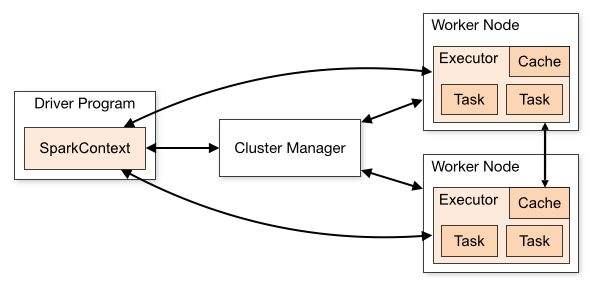
\includegraphics[width=\textwidth]{figures/spark-cluster.png}
    \caption{
      Schematics of a Spark cluster with two workers, each of them with one exectuor and two threads per executor.
      Source: Apache Spark Documentation, https://spark.apache.org/docs/latest/cluster-overview.html
    }
    \label{fig:spark-cluster}
\end{figure}

In Spark, each physical machine is called a \textit{worker}.
On each worker, Spark starts one or multiple Spark processes in their own JVM instance; each of them is called \textit{executor}.
Nowadays, many Spark deployments use a single executor per worker\footnote{This is the setup Databricks uses; Databricks is the leading
maintainer of the Spark platform and offers professional deployment to many customers.}.
Each executor runs multiple threads (often one per core on its worker) to execute multiple tasks in parallel.
In total, a Spark cluster can run \textit{\# workers} $\times$ \textit{\# executors per worker} $\times$ \textit{\# threads per executor} tasks
in parallel.

Spark uses two kinds of processes to execute an application: a \textit{driver program} and multiple \textit{executors}.
When started, the driver program acquires resources from the \textit{cluster manager} for its executor processes.
These executors stay alive during the whole Spark application.
Then, the driver program continues executing the Spark application.
When it encounters parallelizable tasks, it schedules them on the available executors.

All tasks scheduled on the same executor share a cache for in-memory data structures like \textit{Broadcast variables} or persisted RDD
partitions.
This is important in the context of this thesis because it means that we cache the input graph once per executor;
which in many Spark deployments is once per worker or physical machine.
This would not be possible if different tasks in the same JVM would not share the same cache.

Spark allows the user to choose a cluster manager to manage resources in the cluster.
It comes with good integration for Hadoop YARN~\cite{yarn}, Apache Mesos~\cite{mesos} and Kubernetes~\cite{kubernetes}, as well as,
a standalone mode where Spark provides its own cluster manager functionality.
Finally, one can run Spark on a single machine in \textit{local mode}.
In local mode, the driver program and a single executor share a single JVM.
The executor uses the cores assigned to Spark to run multiple worker threads.
For our experiments, we run Spark purely in local mode.

\subsubsection{Catalyst} \label{subsubsec:catalyst}
Catalyst~\cite{spark-sql} is Spark's query optimizer.
It can process queries given as a SQL string or described using the DataFrame API.
From a given query it constructs an executable \textit{physical plan}.
The query compilation process is organized in multiple stages.
Its inputs and stages are shown in~\cref{fig:catalyst-stages}.
Below we explain these in order.
We use the triangle given by the datalog rule $COUNT(triangle(A, B, C)) \leftarrow R(A, B), S(B, C), T(A, C), A < B < C $ as
a running example.

\begin{figure}
    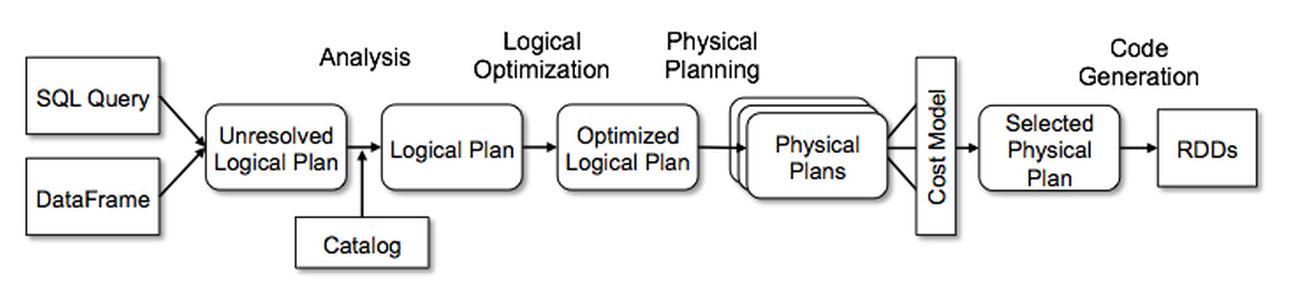
\includegraphics[width=\textwidth]{figures/catalyst-stages.png}
    \caption{
    Input and stages of the Catalyst optimizer.
    Source: Databricks Blog, https://databricks.com/blog/2015/04/13/deep-dive-into-spark-sqls-catalyst-optimizer.html
    }
    \label{fig:catalyst-stages}
\end{figure}

The input of Catalyst is a query in the form of a DataFrame or SQL string.
From this the optimizer builds a \textit{unresolved logical plan}.
This plan can include unresolved attributes, e.g. attribute names which are not matched to a specific
data source yet or which have no known type.
To resolve this attributes Catalyst uses a \textit{Catalog} of possible bindings which describe the
available data sources.
This phase is referred to as \textit{Analysis} and results in a \textit{logical plan}.
The logical plan represents \textit{what} should be done for the query but not exactly \textit{how},
e.g. it might contain a Join operator but not a Sort-merge join.

We show the logical plan for the triangle query in~\cref{fig:triangle-logical-plan}.
As we see, the query is represented as tree where the vertices are operators and the edge indicate dataflow from
one operator to another.
The leaves of the tree are three aliases of the edge relationship.
Two of these source relationships are the input the join between \textit{R} and \textit{S} via \textit{B}.
The result of this join and the leaf relationship \textit{T} are input to the second join.
The tuples produced by this join are filtered to fulfil $A < B < C$.
Finally, at the root of the tree, there is an aggregation to count all results and report the sum.

\begin{figure}
    \centering
    \subfloat[Logical plan\label{fig:triangle-logical-plan}]{\includesvg[width=0.4\textwidth]{triangle-logical-plan}}
    \subfloat[Physical Plan\label{fig:triangle-physical-plan}]{\includesvg[width=0.6\textwidth]{triangle-physical-plan}}
    \caption{Logical and physical plan for the triangle count query as generated by Catalyst.}
\end{figure}

The \textit{logical optimization phase} applies batches of rewriting rules until a fixpoint is reached.
A simple example of a logical optimization would be rewriting $2 + 2$ into $4$.
In the running example of the triangle query, this phase pushes the filters into the two joins.
This optimization is called Filter Pushdown.
It is efficient because it applies filters earlier within the pipeline reducing the number tuples to process by later operators.

From the \textit{optimized logical plan} the optimizer generates one or multiple \textit{physical plans} by
applying so called \textit{Strategies}.
They translate a logical operator in one or multiple \textit{physical operators}.
\textit{Strategies} are also allowed to return multiple physical plans for a single \textit{logical plan}.
In this case, the optimizer selects the best one according to a \textit{cost model}.

The physical plan for the triangle query is shown in~\cref{fig:triangle-physical-plan}.
We see multiple examples of translation of a logical operator, which describes what to do, to its physical pendant that also
describes how to do it: the \textit{TableScan} becomes a \textit{CSVRead} and the \textit{Joins} are implemented as
\textit{BroadcastHashJoins}.

Furthermore, we see the introduction of exchanges.
\textit{BroadcastExchanges} precede the \textit{BroadcastHashJoins}.
They build a hashtable from their input operators and make them available as a broadcast variable to all executors of the cluster;
we explain broadcast variables in depth in~\cref{subsubsec:broadcast-variables}.
When an executor is tasked to execute the hash join operator, it acquires the broadcasted hashtable and executes a local hash join
of its assigned partitions.

Another exchange operator is introduced for the aggregation.
It is broken up into a partial aggregation directly after the last join, an exchange reorganizing all partial counts into a single
partition and a second aggregation over that partition to calculate the total count.
The last is a good example of Catalyst introducing a shuffle.

To conclude, the translation to a physical plan translates logical operators into concrete implementations of these and adds exchanges
to organize the data such that it can be processed independently in partitions.

After generating and choosing a physical plan, Catalyst enters the \textit{code generation} phase in which it compiles Java byte code for
some of the physical operators.
This code executes often magnitudes faster than interpreted versions of the same operator~\cite{spark-sql} because
it can be specialized towards this particular query, e.g. if a join operates only on integers, code
generation can prune all code paths dealing with strings.
Indeed, the code generation phase is part of another Spark project called
\textit{Tungsten}~\cite{tungsten-project,tungsten-code-generation}.
In this thesis, we do not build any code generated physical operators.
Hence, we do not treat this topic in depth.
It is enough to know that all freshly generated Java code is wrapped into a single physical operator.
Therefore, it integrates seamlessly with interpreted operators.

Finally, Catalyst arrives at an optimized physical plan which implements the query.
The execution of this plan is called
\textit{structured query execution}~\cite{spark-internals-structured-query-execution}.
It translates the plan into RDD operations implemented by Spark's core.
Hence, the result of Catalysts query compilation is an RDD representing the query.
One should note that structured query execution does not materialize the query: the result is an RDD which is a none
materialized representation of the operations necessary to generate the result.
In this thesis, we are not concerned with the internals of RDD's.
We do not need to introduce any new RDD operations or even touch Spark's core functionality.
Thanks to the extensibility of Catalyst, we can integrate worst-case optimal joins by adding one logical operator, multiple
physical operators and a Strategy to translate between them.

\subsubsection{Broadcast variables} \label{subsubsec:broadcast-variables}
\textit{Broadcast variables} readonly variables which are accessible by all tasks.
They are initialized once by the driver program and should not be changed after initialization.
The process of broadcasting them is handled by Spark.
It is guaranteed that each broadcast variable is sent only once to each executor and allows it to be spilled to disk if it is not
possible to keep the whole value in memory.
Furthermore, `Spark attempts to distribute broadcast variables using efficient broadcast algorithms to reduce communication
costs'~\cite{rdd-programming-guide}; currently Spark uses a BitTorrent-like communication protocol\footnote{See Spark sources:
\texttt{org.apache.spark.broadcast.TorrentBroadcast}}.
Once sent, they are cached once per executor~(see also~\cref{subsubsec:spark-architecture}) and shared by all tasks on this executor.
They are cached in deserialized form in memory but can be spilled to disk if they are too big.
In this thesis, we use broadcast variables to cache the edge relationship of the graph on all workers.

\subsection{Worst-case optimal join algorithm}\label{subsec:worst-case-optimal-join-algorithm}
The development of worst-case optimal joins started in 2008 with the discovery that the output size of a relational query
is bound by the fractional edge number of its underlying hypergraph~\cite{agm}.
In short, this bound proves that traditional, binary join plans perform asymtopically worse than theoretical possible
for the worst-case database instances, e.g. heavely skewed instances.
For instance, the worst-case of the triangle query is in $\mathcal{O} (N^2)$ , while the AGM bound
shows the possibility to solve it in $\mathcal{O} (N^{3/2})$.
The AGM bound has been treated widely in literature~\cite{skew-strikes-back,andreas,agm}.
A particular good explanation is given by Hung Ngo et al in~\cite{skew-strikes-back}.
We refer the reader to these papers for further information.
In the next paragraph, we discus different algorithms matching the AGM bound which are called worst-case optimal joins.

In 2012, Ngo, Porat, Re and Rudra published a join algorithm matching this bound~\cite{nprr}, called \textit{NPRR} join.
In the same year, Veldhuizen proved that the algorithm \textit{Leapfrog Triejoin} used in LogicBlox,
a database system developed by his company, is also worst-case optimal with regards to the fractional edge number bound.
We often abbreviate Leapfrog Triejoin to \textsc{LFJT}.
Both algorithms have been shown to be instances of a single algorithm, the \textit{Generic Join}, in 2013 Ngo et al.~\cite{skew-strikes-back}.

We identified three worst-case optimal join algorithm: NPRR, LFTJ and Generic Join.
We choose Leapfrog Triejoin as the basis for our work.
The argumentation for this decision is given below.
First, we identify the main criteria this choice.
Then, we use them to compare the different algorithms.

The most important argument for our decision is the degree to which the algorithm has been shown
to be of practical use.
In particular, the number of systems it is used in and openly available data on its performance.
If an algorithm is used in academia as well as in industry, we deem this as a big advantage.
This criteria carries a lot of weight because the first literature on worst-case optimal joins
has been rather theoretical but in our work we take a more praxis and system oriented perspective.

The practical character of our work also motivates the second dimension we compare the algorithms in, namely
ease of implemenation.
If two of the three algoritms both have well proven performance, we would like to choose the algorithm
that takes less time to implement and is easier to adapt and experiment with.
That is to be able to spent more time on evaluation and optimizations for the graph use-case, instead of,
time spent on replicating existing work.

The Leapfrog Triejoin is used in two commercial database solutions:
LogicBlox~\cite{logicBlox} and RelationalAI~\footnote{https://www.relational.ai/}.
Its performance has been reported on in two publications~\cite{myria-detailed,olddog}.
In particular, it beats various general and graph specific databases for graph pattern matching~\cite{oldgo}, i.e.
PostgresSQL, MonetDB, NEO4J, graphLab and Virtuoso.
The broadest study of its performance uses 15 different datasets and 7 queries~\cite{olddog}.
We conclude that the performance of \textsc{LFTJ} is well established by peer reviewed publications
as well as industrial usage.
% TODO find cites for graphlab and Virtuoso

\textit{NPRR} has been well analyzed from the theoretical point of view.
However, we are not able to find any openenly available sources with performance measurements.
This disqualifies \textsc{NPRR} as basis for our thesis.

\textit{Generic Join} is used in at least three academic graph processing engines,
namely GraphFlow~\cite{graphflow}, EmptyHeaded~\cite{emptyheaded} and a unnamed implemenation in
Timely DataFlow~\cite{ammar2018distributed}.
All three show good performance.
However, we are not aware of any commercial systems using \textsc{GJ}.

The comparision of Leapfrog Triejoin, \textsc{NPRR} and \textit{Generic Join} by proven performance
rules out \textsc{NPRR} and puts \textsc{LFTJ} and \textsc{GJ} on a similar level.
Next, we compare these two algorithm in ease of implementation.

The description of the Leapfrog Triejoin implementation in its original paper~\cite{lftj} is excellent.
Furthermore, multiple open source implementation exists~\cite{de-witt,myria-detailed}.
In particular, the implementation of Christian Schroeder for a course at Oxford is helpful because it is standalone and
does not require us to understand a whole system\footnote{TODO GitHub Dewitt}.

\textit{Generic Join} is described as a generalization of \textsc{NPRR} and Leapfrog Triejoin in its original
paper~\cite{skew-strikes-back}.
Although, well written and algorithmically clear, this explanation is much less practical than the one given for \textsc{LFTJ} which
is backed by a executable implementation.

To conclude, we choose Leapfrog Triejoin as basis for our work based on its openely available records of performance, use in
academic as well as industrial systems and good description for direct implementation.
Furthermore, Peter Boncz (supervisor of this thesis) has direct contact to the inventors of \textsc{LFTJ} giving us access to valuable
expertise if necessary.

\subsubsection{LeapfrogTriejoin}
% Use in industry
The Leapfrog Triejoin gives strong theoretical guarantues which have been proven to be worst-case optimal in~\cite{lftj}.
Moreover, the \textsc{LFTJ} has been shown to be of practical use in multiple systems and papers.
It is at the core of the commercial LogicBlox database system~\cite{lftj} and in the products of
RelationalAI\footnote{https://www.relational.ai/}, the latter company of its inventors.
Hence, showing its worth in industry.
In academia, Leapfrog Triejoin has been shown to beat traditional binary join plans employing Hashjoins or Sort-Merge joins,

% background over "typical" graph pattern matching queries needed
%   olddog good introduction about binary joins vs wcoj for graph pattern matching
% background about graph pattern matching needed

% WCOJ against graph engines (oldog)

% worst case optimal up to a logN modulo, can be eliminated lftj
%  more optimal than NPRR on some instances (see lftj)

% Queries in terms of full conjunctive queries, existence queries, none-equi joins
%   extensions to disjunctions, ranges, negation and projection discussed in LFTJ

% background on binary join operators?
% comparision, intermediate results
%  intuitive understanding of why better?

% Queries: olddog, Semih's paper,
%    Mostly for graphs
% Comparision with other systems: oldog, graphlab, virtuoso, monetdb, pssql, neo4j


% Variable ordering: Semih's paper, lftj, design of logixblox: Optimization and parallelism.


% Algorithm and Implemenation
%    As layered algorithm LFTJ, LF, TrieIterators
%    performance guaruntues of the different layers
%    different backing datastructures B-Trees, Arrays Tributary join.
%       in this work we add CSR
%    Connection to query should stay clear, that's why LFTJ paper chooses to introduce them bit
%    by bit


% Codegeneration studied by RelationalAi
% Compression studied by Richard


% Query assumptions
%    Each variable at most once per argument list
%    Each argument list must be a subsequence of the variable ordering

\subsection{Distributed worst-case optimal join in Myria} \label{subsec:myria}
In 2014, a Leapfrog Triejoin variant, dubbed ``Tributary Join'', was used as a distributed join algorithm on a shared-nothing architecture called ``Myria''~\cite{myria-detailed}.
They use Tributary Join as a local, serial worst-case optimal join algorithm, combined with the Hypercube shuffle algorithm to partition the data between their machines~\cite{hypercube}.
% TODO sort out hypercube and shares usage
However, it is not obvious how well Hypercube shuffles scales because it replicates many of its input tuples~\cite{myria-detailed}.
The combination of Hypercube shuffles and Tributary Join in Myria does not scale well (speedup of 8 on 64 workers compared to the time it takes on 2 nodes) which, although unlikely to be optimal, is not investigated in great detail; we therefore, explain Hypercube shuffles in detail and show that they tend to replicate all data to all nodes for bigger graph patterns~\cref{ssec:hypercube-shuffle}.
Their approach is directly applicable to Spark.
% TODO add Graphflow paper: variable ordering studied, combination of bin + wcoj in plans, query planning first known approach, parallel
% execution?
% TODO check emptyheaded, it uses WCOJ's

\subsubsection{Shares}
% TODO rename HC Shares
We first explain how the Hypercube shuffle algorithm, \texttt{HC}, partitions data.
After, we provide an analysis of its scaling with regards to graph patterns with an increasing number of vertices.

\texttt{HC} partitions the input relationships for a multi-way join over \textit{w} worker nodes, such that, all tuples, which could be joined, end up on the same worker in a single shuffle round.
Hence, it allows running any multi-way join algorithm locally after one shuffle round.
The output of the join is the union of all local results.
\texttt{HC} realizes this partitioning by logical organizing all workers in a hypercube with one dimension per join variable; we call the number of variables \textit{A} and use $a_i$ to reference a single variable.
Each dimension has a size $p_i$, the $p_i$'s have to be chosen such that the constraint $w \ge \prod_{i}p_i$ is satisfied.  % TODO choosing problem
In other words, each worker can be addressed by its coordinate in the hypercube of the form $\{1..p_1\} \times ... \times \{1..p_A\}$.

With this topology in mind, it is straightforward to find a partitioning for all tuples from all relationships such that tuples that could join are sent to the same node.
We choose a hash function $h_i$ for each join variable which maps its values in the range of \{1..$p_i$\}.
Then each worker determines where to send the tuple it holds by hashing its join variables.
This results in a coordinate in the hypercube which is fixed for all join variables, which occur in the tuple, and unbounded for join variables not bound by the tuple.
Then the tuple is sent to all workers with a matching coordinate.
For example, assume a join with three variables $a_1$, $a_2$ and $a_3$ and tuple \textit{t} that binds $a_1$ and $a_2$ then we get the coordinates $h_{a1}(t_{a1}) \times h_{a2}(t_{a2}) \times \{0..p_{a3}\}$ and send the tuple
to all workers with a coordinate matching the first two attributes and arbitrary third component of the coordinate; the tuple is replicated across $p_{a_3}$ machines.

Next, we analyse the scalability of \texttt{HC} on growing graph patterns - that is, joins over a single relationship, the edge relationship of the graph \textit{E} and with two variables per atom.
In this context, atoms of the join can be seen as the edges of the pattern and variables as vertices.
In the following we consider the join query represented by the Datalog rule $Q(a_1, ..., a_A) = R_1(a_1, a_2), ..., R_k(a_{A-1}, a_A)$, we call $atoms(Q)$ the set of all atoms in $Q$, $p_1(R)$ and $p_2(R)$ the $p_i$ corresponding to the variables of $R$.
We use the method described in~\cite{myria-detailed} to calculate optimal shares allocation $p_1 ... p_A$.

Each worker receives $\sum_{R \in atoms(Q)} |R| / (p_1(R) * p_2(R))$ tuples under the assumption of uniform data distribution and good hash functions.
Our argument is that the tuples of each $R$ are divided onto $p_1(R) * p_2(R)$ workers - the workers that form the hypercube planes of its two variables.

In the special case of graph pattern matching where all atoms of the query are pointing to the same relationship, we can optimize \texttt{HC} shuffle such that a tuple is only sent once to a worker, although it might be assigned to it via multiple atoms.
If we apply this optimization, we can predict the probability with which each tuple is assigned to a worker using the Poisson binomial distribution.
The Poisson binomial distribution $Pr(n, k, u_0, ..., u_n)$ allows us to calculate the likelihood that $k$ out of $n$ independent, binary and differently distributed trials succeed, under the condition that the $i$'th trial succeeds with a probability of $u_i$.
We then use $n = |atoms(Q)|$, $k = 0$ and $u_i=1/(p_1(R_i) * p_2(R_i))$ to calculate the probability that a tuple is not assigned to an arbitrary, fixed worker $w$.
This allows us to predict the number of tuples assigned to each worker by $|E| * (1 - Pr(|atoms(Q)|, 0, u_0, ..., u_{|atoms(Q)|})$.

\Cref{table:workload} shows the expected percentage of tuples from $E$ assigned to each node for graph patterns of different sizes calculated using Poison binomial distribution and optimal shares assignments according to the method used in~\cite{myria-detailed}.
As we can see in this table, the number of tuples assigned to each worker grows over linear in the size of the graph pattern and that doubling the number of workers is inefficient to counter this growth.

The second observation has two reasons.
First, doubling the number of workers does not allow to double the dimensions of the hypercube - a hypercube always needs $p_1 \times ... \times p_A$ workers to be built.
Second, the number of replicated tuples increases with a growing hypercube because each tuple from $R_i$ is replicated to $\prod_{R_j \in atoms(Q)/R_i} p_1(R_j) * p_2(R_j)$; due to the fact that each tuple binds only two out of $A$ variables the tuple is replicated over many dimensions, e.g. let the bounded varibales be $a_p$ and $a_s$ then we get  $|\{0..p_0\} \times ... a_p ... \times ... a_s... \times \{0..p_A\}|$ matching worker coordinates.


%First, a hypercube of size $s$ and $A$ dimensions requires $s^A$ workers.
%Second, the replication increases with $A$ and $s$; we argue that each tuple is replicated to $(s+1)^{A-2}$ workers.
%Each tuple binds two out of $A$ variables, let's assume these are $a_p$ and $a_s$ then we have $|\{0..s\} \times ... a_p ... \times ... a_s... \times \{0..s\}|$ matching worker coordinates\footnote{The argument can be rephrased as the number of all strings of the length $A-2$ over the alphabet $\{0..s\}$}.

\begin{table}[t]
    \centering
    \begin{tabular}{lrr}
        \toprule
        Pattern  & Edges  & workload [64]/[128] \\ \midrule
        Triangle & 3                 & 0.18 / 0.12    \\
        4-clique & 6                 & 0.59 / 0.44    \\
        5-clique & 10                & 0.9  /d 0.82    \\
        House    & 5                 & 0.42 / 0.32    \\
        Diamond  & 8                 & 0.76 / 0.67    \\
        \bottomrule
    \end{tabular}
    \caption{Workload, on 64 and 128 workers, in percentage of tuples of the edge table assigned to each worker, using Poison binominial distribution to estimate the workload and the method from~\cite{myria-detailed} to determine the optimal shares configuration.}
    \label{table:workload}
    % See hc-workload-1.csv computed with a28fc458f4f8959a5af81a65f593ea22dcb8dd44
\end{table}

In light of the numbers presented in \cref{table:workload} and in line \cite{ammar2018distributed}, we conclude that the communication costs for \texttt{HC} converge towards a full broadcast for bigger graph patterns and scaling becomes increasingly inefficient.
Anyhow, \texttt{HC} is proven to be communication cost optimal for general multi-way joins in map-reduce like systems in a single round of shuffling in multiple settings~\cite{beame2013,beame2014,beame2016}.
Therefore, we decide to follow a different direction for distributing WCOJ's which we explain in~\cref{sec:goals}.


\subsection{Analysis of public real-world graph datasets}\label{subsec:graph-analysis}
TODO will include histogram of graph sizes, average outdeegree, maybe clustering coefficient and further interesting metrics, with
regards to the thesis, for (all?) graphs of the SNAP and Labaratory of Web Algorithms dataset collection.

\subsection{Compressed sparse row representation}\label{subsec:csr-background}
Compressed sparse row representation (short CSR) is a well known, low-memory representation for static graphs~\cite{csr,csr-first}.
To ease its explanation, we assume that the graph's vertices are identified by the numbers from 0 to $|V| - 1$.
However, our implementation allows the use of arbitrary vertice identifiers in $\mathcal{N}$ by storing the translation in an additional
array of size \textit{|V|}.

CSR uses two arrays to represent the edge relationship of the graph: one of size \textit{|E|} which is a projection of the edge relationship
onto the \textit{dst} attribute and a second of size \texttt{|V + 1|} which stores indices into the first array.
To find all destinations directly reachable from a source \textit{src $\in$ V}, one accesses the second array at \textit{src} for the
correct index into the first array for a list of destinations.
% TODO maybe example figure?

The CSR format has two beneficial properties in the context of this thesis.
First, it allows locating all destinations for a source vertice by one array lookup;
hence, in constant time.
Second, the representation is only, roughly, half as big than a simple columnar representation.
A uncompressed columnar representation needs $2 \times |E|$ while CSR uses only $|V| + 1 + |E|$, note that for most real-world graph |V|
<< |E| holds (see~\cref{subsec:graph-analysis}).



% Parallelism in Spark
% ====================
%We give examples for both kind of parallelism in the triangle count query
%(\cref{fig:lineage-triangle}).
%Lets assume that the CSV file is partitioned in 10 equal parts and each part is read
%by one out of 10 workers.
%Then the resulting RDD has 10 partitions.
%The following filter can be applied to all 10 partitions in parallel.
%This computation is also task parallel because all three filters can be applied to the
%input set directly after reading it from disk.

%If we go one step further into the example of the triangle query and look at the first
%join, we see limitations to Spark's parallelism.
%Let's assume that we want to use a Hashjoin implementation.
%In this case, we have to build a hash table of either side of the join.
%Hence, the computation of the join needs to wait until this hash table has been build.
%This is clearly not task parallel and it's also not data parallel on the build site
%because we need the data from all partitions to construct a full hash table.
%The result is that we see an exchange operator in the DAG of \cref{fig:triangle-lineage}.
%This operator allows to reorganize the partitions of a RDD.
%In the case of a hash join, it would reorganize items from all partitions into a hash
%table and make copies of this hash table available to the tasks that compute the
%partitions of the join.

%In the last paragraphs, we covered that Spark uses data parallelism arising from the partitioning of the RDD's
%and task parallelism arising from the lineage-graph representation of the RDD's.
%Synchronization happens via exchange operators which allow to reorganize the paritioning of the RDD's.
%In the following, we explain how Spark exploits parallelism in its execution model.

%Spark uses a scheduler to assign \textit{tasks} to \textit{slots}.
%\textit{Tasks} are the smallest unit of work in Spark.
%They are created by dividing the RDD lineage graph into pipelinable \textit{stages}.
%Normally, a stage consists out of all transformations between two exchange operators.
%Each stage consists out of as many tasks as it has partitions.

%The stages of the triangle query are shown in \cref{fig:triangle-lineage}.
%We have four stages.
%Two to build the hash table for our hash join which start with reading the CSV from disk and end with the exchange operator before
%the join.
%The longest stage also reads the CSV from disk, includes the two streaming sites of the hash joins and finally aggregates all
%results per partition for the count.
%It ends with an exchange to aggregate the counts of all partitions; this aggregation is the last out of for \textit{stages}.
%
%These four stages lead to 31 tasks if we assume that each stage starts with reading the CSV into 10 partitions.
%This is because the first 3 stages have 10 tasks each and the last stage accumulating all counts after the last task is only as single
%task of summing up all partitions of its parent.

\section{Worst-case optimal join parallelization}  % TODO header

Based on the fact that Shares is an optimal partitioning scheme for n-ary joins in MapReduce like systems~\cite{shares} and
our analysis that Shares converges to a full broadcast of the graph edges (see \cref{shares-proof}), we decided
to forego physical partitioning of the graph.
We cache the graph in memory such that each Spark task can access the whole graph.
Then, we experiment with multiple \textit{logical} partitioning schemes which ensure that each task processes
only some parts of the graph.

This design allows us to implement a new flavour of the Shares partitioning in which we filter the vertices of the
graph on-the-fly while processing it with our \textit{Graph\textsc{WCOJ}} algorithm.
We describe this contribution in \cref{ssec:shares-logical}.

Furthermore, we consider a work-stealing based partitioning which does not replicate any work and produces less
skew than Shares. % TODO is that always correct.
This comes at the price of implementing work-stealing on Spark.
The design of work-stealing in Spark is described in \cref{ssec:work-stealing}

\subsection{Logical Shares} \label{ssec:shares-logical}
Shares has been developed as a optimal shuffle for n-ary joins on MapReduce like systems.
So, it is used to physical partition the tables participating in the join over all workers of the system.
Then, each worker works only on the tuples it holds in its partition.
This has been implemented in Myria for \textsc{WCOJ}~\cite{myria-detailed} and for Haddoop~\cite{TODO}.
We describe the Shares and Myria in more detail in~\cref{ssec:myria} and assume that the reader is familiar
with this section.

The idea of Shares can also be used for a \textit{logical} partitioning scheme.
Instead, of partitioning the graph before computing the join, we determine if a tuple should be considered by the
join on-the-fly.
We do so by assigning a coordinate of a hypercube to each worker as in the original Shares.
Then each worker is responsible for the tuples which match its coordinate.
However, in the \textsc{LFTJ} we do not consider whole tuples but only single attributes of a tuple at the time,
e.g. a \textit{LeapfrogJoin} only considers one attribute and cannot determine the whole tuple to which this attribute
belongs.
Fortunately, a tuple matches a coordinate if all hashes match the coordinate.
Hence, we can filter out a tuple if any of its attributes does not match.
For example, we can exclude a value in a \textit{LeapfrogJoin} without knowing the whole tuple.

Integrating Shares and \textsc{LFTJ} with each other comes with two important design decisions.
First, the \textit{LeapfrogTriejoin} operates on all tuples.
Hence, we need to filter out the values that do not match the coordinate of the worker.
Second, where to compute the optimal Hypercube configuration.
We describe our solutions below.

% TODO main difference between precomputed filtered relationship and one shared on-the-fly filtered relationship.

The first design decision is where to filter the values.
The \textit{LeapfrogTriejoin} consists out of multiple components which are composed as layers upon each other.
On top we have the \textit{LeapfrogTriejoin} which operates on one \textit{LeapfrogJoin} per attribute.
The \textit{LeapfrogJoins} uses multiple \textit{TrieIterators}.
Our first instinct is to push the filter as deep as possible into these layers.

We built a \textit{TrieIterator} that never returns a value which hash does not match the coordinate.
This is implemented by changing the \textit{next} and \textit{seek} methods such that they linearly
consider further values until the they find a matching value.
However, the resulting \textsc{LFTJ} was so slow that we abundant this idea immediately.
We hypothize that this is the case because the original \textit{next} and \textit{seek} method is now followed
by a linear search for a matching value.
Furthermore, many of these values are later dropped in the intersection of the \textit{LeapfrogJoin} which
can also be seen as a filter over the values of the \textit{TrieIterators}.
As we know from~\cref{ssec:leapfrog-materialization}, the \textit{LeapfrogJoin} is a rather selective filter.
It does not make sense to push a less selective filter below a more selective filter.

With this idea in mind, we build a logical Shares implementation that filters the return values of the \textit{leapfrogNext}
method.
This is implemented as decorator pattern around the original \textit{LeapfrogJoin}.
The use of the decorator pattern allows us to easily integrate Shares while at the same time allows for
other partitioning schemes later on.

% TODO to negative?
The second design decision is how and where to compute the best hypercube configuration.
The how has been discussed extensively in former literature~\cite{shares,myria-detailed}
% TODO there's one or two more papers, see myria-detailed
We implement the exhaustive search algorithm used in the Myria system~\cite{myria-detailed}.
%In their paper they conclude that this is a `practical and efficient' solution.
%Given that the computation of the hypercube configuration can cost up to 45s for 96 workers, this is only
%the case for quite long running queries.

In interest of a simple solution, we compute the best configuration on the master before starting the Spark
tasks for the join.
We note that the exhaustive algorithm could be optimized easily and it would be worthwhile to introduce
a cache for common configurations.
Due to time constraints, we leave this to future work and keep our focus on the scaling behaviour of Shares.

To conclude, we succeeded to integrate Shares with \textit{LeapfrogTriejoin} and report our results in \cref{ssec:graphWCOJ-scaling}.
We cannot improve on the main weakness of Shares that it duplicates a lot of work.
Indeed, our design filters out tuples only after the \textit{LeapfrogJoin}.
Therefore, all tuples are considered in the \textit{TrieIterator} and their binary search.
However, we are able to share the same CSR data structure for all \textit{TrieIterator} and do not
need to materialize a prefiltered data structure for each \textit{TrieIterator} which saves time and memory.

\subsubsection{RangeShares}
In the last section, we raised the point that our Shares implementation only filters out value after the
\textit{LeapfrogJoins}.
This is due to the fact that the hash based filter of Shares filters values one-by-one.
In this section, we explore the possibility to use range based filters which can be pushed into the \textit{TrieIterators}.
However, we warn the reader that this is a negative result.
It leads to high skew which hinders good scaling of this idea.




\subsection{Work-stealing} \label{ssec:work-stealing}

\section{Graph\textsc{WCOJ}} \label{sec:graphwcoj}

\subsubsection{Combining \textsc{LFTJ} with \textsc{CSR}}
For our graph pattern matching specialized \textit{LeapfrogTriejoin} version we choose \textsc{CSR} (see \cref{subsec:csr-background}) as
backing data structure.
This data structure is typically used for static graphs and we show that it is a great match for \textsc{LFTJ}.
In this section, we shortly describe the implementation of a \textsc{CSR} based \textit{TrieIterator}, point out the differences between
this new version and a column based \textit{TrieIterator} (as described in~\cref{ssec:seq-implementation}\footnote{To be rewritten and
integrated}) and conclude with an experiment demonstrating the power of this optimization.
% TODO rewrite and integrate with LFTJ chapter

The implementation of a \textsc{CSR} based \textit{TrieIterator} is straightforward except for one design change: instead of using
the vertice identifier from the graph directly, we use their indices in the \textsc{CSR} representation.
This change is rather minor because it can be contained at any level by using a hash map for translation, e.g. in the
\textit{TrieIterator} itself, in the \textit{LeapfrogTriejoin} or at the end of the query by an additional mapping operation.
In the current system, the translation is performed by the \textsc{LFTJ} implementation to allow easy integration into other projects.
However, it is possible to work on the indices throughout the whole system to safe the translation costs.
We now outline how to implement each of the \textit{TrieIterator} methods, under the assumption that all vertices have outgoing edges.
Then, we drop this assumption and explain the necessary changes.
The creation of the \textsc{CSR} data structure itself is described in~\cref{subsec:csr-spark}\footnote{To be
written.}.
% TODO CSR creation

We use the variables \textit{depth}, \textit{srcPosition} and \textit{dstPosition} to store if we are operating on the source or destination
level and the positions of the iterator on the respective level.
We call the two arrays of the \textsc{CSR} datastructure \textit{dst} for the array storing all edge destinations and \textit{dstIndices}
for the array storing indices into \textit{dst} (refer to \cref{ssec:csr-background} for a complete explanation of these arrays).
The \textit{open} function does nothing if we open the first level; if we open the second level, it sets \textit{dstPosition} to
\textit{dstIndices(srcPosition)}.
Additionally, it updates \textit{depth}.
The \textit{up} function only updates \textit{depth}.
The \textit{next} method increases \textit{srcPosition} or \textit{dstPosition} by one depending on \textit{depth}.
The \textit{seek(key)} method sets \textit{srcPosition} to \textit{key} if \textit{depth} equals 0 or uses binary search to find
\textit{key} in \textit{dst.slice(dstPosition, dstIndices[srcPosition + 1])} and then sets \textit{dstPosition} accordingly.
The \textit{key} function returns \textit{srcPosition} on the first level and \textit{dst[dstPosition]} if \textit{depth} equals 1.
The \textit{atEnd} function is: \textit{if (depth == 0) srcPosition == dstIndices.length - 1 else dstPosition == dstIndices(srcPosition +
1)}.

<Alternative representation of the \textit{TrieIterator} implementation as table. Let me know what you prefer. I think the text is better
after seeing both.>
\begin{table}[H]
\begin{tabular}{@{}lll@{}}
\toprule
Method    & 1st level                           & 2nd level                                                                                       \\ \midrule
open      & update depth                        & dstPosition $\leftarrow$ dstIndices{[}srcPosition{]}; update depth                              \\
up        & update depth                        & update depth                                                                                    \\
next      & srcPosition++                       & dstPosition++                                                                                   \\
seek(k) & srcPosition $\leftarrow$ k            & dstPosition $\leftarrow$ lub(k, dst[dstPosition:dstIndices[srcPosition +1]] \\
key       & srcPosition                         & dst{[}dstPosition{]}                                                                            \\
atEnd     & srcPosition = dstIndices.length - 1 & dstPosition = dstIndices(srcPosition + 1)\\
\bottomrule
\end{tabular}
\caption{Tabular summary of \textit{TrieIterator} implementation based on \textsc{CSR}. \textit{lub} is \textit{leastUpperBound}.
\textit{dst[<start>:<end>]} slices the array.}
\end{table}

To resolve the assumption of no empty outgoing adjacency lists, we adapt \textit{open}, \textit{next} and \textit{seek} to skip source
positions without outgoing edges.
This is easy to detect because then \textit{dstIndices(x) == dstIndices(x + 1)}.
We can skip these cases by simple linear search until we find a valid position.
This solution is sufficient because there are only a few vertices with no outgoing edges in real-world graphs.
% TODO add to graph analysis chapter?

The \textit{TrieIterator} implementation based on \textsc{CSR} is much faster than the column based iterator; mainly due to the fact
that the \textit{seek} method on the first level can be implemented in $\mathcal{O}(1)$, instead of $\mathcal{O}(\log n)$.
This optimization has huge potential because these searches are the most costly operations for a column based
\textit{TrieIterator}~\cite{myria-detailed}.
Note that searches on the second level are fast, due to the fact that most graphs have a low outdegree (see
\cref{subsec:graph-analysis}).
Additionally to this advantage, \textsc{CSR} based \textit{TrieIterator} do less bookkeeping because they support only 2 levels and spent
nearly no time on processing \textit{atEnd} for the second level, while a column based \textit{TrieIterator} needs to calculate the
number of outgoing edges for each source vertice in its \textit{open} method, to allow a fast \textit{atEnd} method).

We conclude that \textsc{CSR} based \textit{TrieIterator}'s are a promising match for \textsc{LFTJ} and graph pattern matching.
The improvements of this optimization can be seen in \cref{fig:wcoj-vs-graphWCOJ}.
It demonstrates an up to 2.6 speedup over a column based \textsc{LFTJ}. % NUMBER
We also see that the optimization has a stronger impact on queries with more edges and vertices, e.g. \texttt{5-clique}.
For a more thorough evaluation refer to the experiment section \ref{sec:experiments}.

\begin{figure}
\centering
\includegraphics[width=0.5\textwidth]{wcoj-vs-graph-wcoj.png}
\caption{Barchart comparing join time of \texttt{WCOJ} and \texttt{GraphWCOJ} on multiple queries on \texttt{SNB-sf1}}
\label{fig:wcoj-vs-graphWCOJ}
\end{figure}


\subsubsection{Exploiting low average outdegrees}
% TODO study in background

In our study of real-world graphs (\cref{sec:graph-analysis}), we show that most real-world graphs have a small, average outdegree.
The outdegree over all graphs is TODO and the maximum average outdegree of a single graph
is TODO at TODO.
These results lead to the hypothesis that the intersection of multiple adjacency lists is small, e.g. below 10 in many cases.
We can exploit this fact by materializing the intersections in the \textit{Leapfrog joins} directly
in one go; instead of, generating one value at-the-time in an iterator like fashion as described in the
original paper~\cite{leapfrog}.
% TODO rename reference to leapfrog-triejoin
This is beneficial because it makes better use of data locality; we elaborate this statement in a later
paragraph.

We structure the remainder of this section as follows.
First, we shortly reiterate the most important facts about \textit{Leapfrog joins} for this chapter (TODO just organize both sections
behind each other?).
Second, we analysis the intersection workload in terms of input sizes and result size to confirm our hypothesis
and gain valuable insights to choose the best intersection algorithm.
Third, we explain the algorithm we chose based on the analysis.
Fourth, we point out differences to the original Leapfrog Triejoin.
Finally, we present a short experiment showing the performance gains of this optimization.

% TODO synchronize with new Leapfrog section
\textit{Leapfrog joins} build the intersection between multiple adjacency lists.
This is done in an iterator-like fashion in their \textit{leapfrog\_next} method by repeatedly finding the upper-bound for the largest
value in the lowest iterator.
This algorithm is asymptotically optimal for the problem of n-way intersections.
However, we claim that it is (1) to complex for small intersections and (2) should generate all values at once instead of one-by-one to
improve performance on real-world adjacency lists.

To determine the best algorithms to build the n-way intersection in the \textit{Leapfrog joins},
we run some experiments to characterize the workload.
Towards this goal, we log the size of the full intersection, the size of the smallest iterator participating
% TODO multiple queries
and the size of the largest intersection between the smallest iterator and any other iterator on 5-clique queries on \texttt{SNB-sf-1}.
\Cref{fig:intersection-workload} depicts these metrics as cumulative histograms.
In the next paragraphs, we point out the most important observations in each of these graphs.

% TODO why is that faster, deeper in maybe on jit code or perf

\Cref{fig:intersection-workload-smallest} shows the size distribution of the smallest iterator, as to be expected for a social network
graph, the outdegree is between 1 and 200.
% TODO background power-law graph
We do not see the long-tail distribution typical for power-law graphs because we choose the smallest iterator out of 5 and even
though there are vertices with a much higher outdegree, the chance of encountering 5 of these in a single intersection is small.
We note that in 80\% of all cases the smallest iterator has a size lower than 80 and above that the distribution slowly increases to 100\%
% NUMBER

\Cref{fig:intersection-workload-smallest-biggest} illustrates the size distribution of intersecting the smallest iterator with any other
iterator, such that the intersection is maximal.
We choose this specific metric to motivate one of our design choices later on.
As for the smallest iterator, some of these intersections are as big as ~200 but most of them are much smaller.
However, unlike for the smallest iterator metric, 80\% of the intersections contain less than 21  elements and the frequency increases to
100\% in a steep curve.
This last observation is even stronger for the size of the total intersection (\cref{fig:intersection-workload-total}):
the size is less than 5 in 80\% of all intersections and increases similarly steep to 100\%.
The maximum is a little lower than 200.

These observations confirm our hypothesis that the size of the intersections is small (below 5) and do not show the same long-tail
distribution as the whole social network graph.
Hence, we can materialize them without running at risk of building big intermediary results.
Furthermore, the experiment shows that optimizing by taking iterator sizes into account is worthwhile but only for the smallest iterator
because
once we start with the smallest iterator the further intersections are small (below 21) in the vast majority of all instances.


\begin{figure}[H]
\centering
\subfloat[Total intersection\label{fig:intersection-workload-total}]{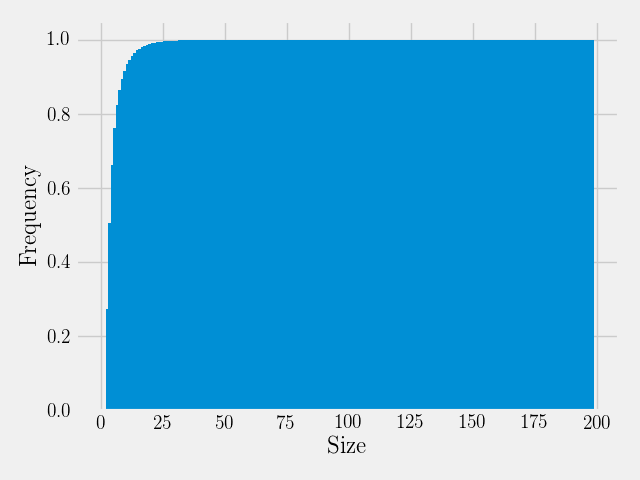
\includegraphics[width=0.3\textwidth]{intersections/total.png}}
\hfill
\subfloat[Largest intersection including smallest iterator\label{fig:intersection-workload-smallest-biggest}]{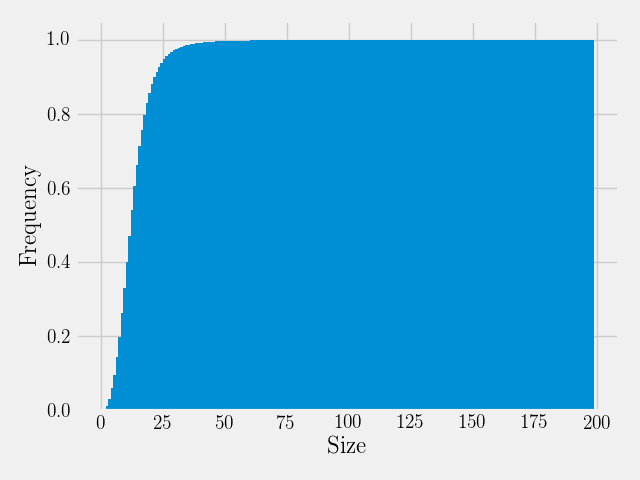
\includegraphics[width=0.3\textwidth]{intersections/smallest-biggest.png}}
\hfill
\subfloat[Smallest iterator\label{fig:intersection-workload-smallest}]{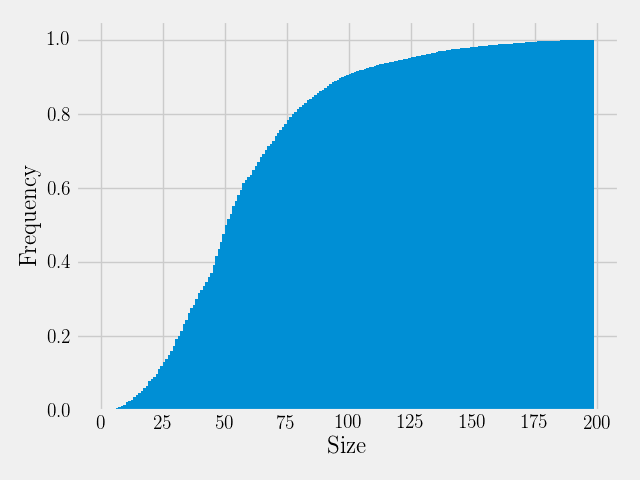
\includegraphics[width=0.3\textwidth]{intersections/smallest.png}}
\caption{Cumulative histograms of total intersection sizes, largest intersection with the smallest iterator and any other, and size of the
smallest iterator participating in \texttt{5-clique} on \texttt{SNB-sf-1}.}
\label{fig:intersection-workload}
\end{figure}

% TODO flowy handover from paragraph to paragraph
In the coming paragraphs, we detail how to build the n-way intersection of multiple adjacency list
such that we gain performance by better use of data-locality than original the \textit{Leapfrog join}.
We choose to use pairwise intersections over multi-way intersection algorithms for their simpler,
linear memory access patterns.

From our analysis, we conclude that the final intersection size is strongly dependent on the
smallest iterator and that the intersection of the smallest iterator with any other iterator is
close to the final size.
These insights translate into two design decisions.
First, we start with the smallest iterator\footnote{We take advantage of the fact that CSR allows us
to determine the size of iterators cheaply (see~\cref{ssec:csr-impl})}.
However, we do not take the sizes of any other iterators into account because the effort for
sorting the iterators by size would not pay off.

Second, we use two different tactics to build the pairwise intersections.
The first intersection between two iterators is built \textit{in-tandem},  where we seek
the upper bound of the higher value in the smaller iterator.
This algorithm guarantees to find the intersection between two iterators in the asymptotical fastest
way.
After this first intersection, the intermediary result is quite small.
Therefore, we use the simpler scheme of linearly iterating the intermediary and probing
the iterator by binary search with fall-back to linear search.

Finally, we point out a few exceptional cases and pitfalls for implementors:
\begin{itemize}
\item If all iterators of the \textit{Leapfrog join} are on their first level, the intersection is near |V|. In this case, we fall back
to the original
\textit{Leapfrog join}.
\item We use an array to materialize the intersections because Scala collections are slow.
Instead of deleting elements, we replace them with a special value.
\item Allocating a new array for every \textit{Leapfrog join} initialization is costly.
We estimate the size of the intersection by the size of the smallest iterator and reuse the array whenever possible. We use a sentry element to mark the end of the array.
\end{itemize}

The carefully chosen operations explained above are faster than the original \textit{Leapfrog join}
algorithm for two reasons.
First, although, the original algorithm uses an asymptotical better n-way intersection, multiple
binary intersections are preferable with the rather small adjacency lists of graph workloads.
In particular, in our situation where the size of the first binary intersection is already
very close to the size of the final intersection.

Second, the \textit{Leapfrog join} generates a single value, then yields control to other parts
of the \textit{LeapfrogTriejoin} algorithm and later touches the same adjacency lists again to generate the next value.
Our approach touches the adjacency lists exactly once per \textit{Leapfrog} initialization and
condenses the intersection into a much smaller array.
This array is more likely to stay cached while the other parts of the \textit{LeapfrogTriejoin} do their work.

\Cref{fig:mat-vs-nomat} shows that a materialized \textit{Leapfrog join} out-performance better than
the original algorithm.
As expected, the optimization is more powerful for bigger queries because they work with more
adjacency lists per \textit{Leapfrog join}, e.g. for a triangle each \textit{Leapfrog join} intersects
only two iterators while for a \texttt{5-clique} each join handles 5 adjacency lists.
Anyhow, even for the triangle query, we see a small but clear improvement and a lower error due to
better cache use.
We refer the reader to our experiment section (\ref{sec:experiments}) for further experiments on
our graph specialized \textsc{wcoj} and detailed descriptions of the datasets and queries used.

\begin{figure}[H]
\centering
% TODO more queries
% TODO add amazon graph
% TODO rename dataset to materialization and no materialization or such
\includesvg[width=0.5\textwidth]{mat-graph-bar-snb-sf1}
\caption{Barchart showing \texttt{GraphWCOJ} with and without \textit{Leapfrog join} materialization
enabled for different queries on \texttt{SNB-sf1}.}
\label{fig:mat-vs-nomat}
\end{figure}
\section{Implementation}\label{sec:implementation}

\subsection{General sequential version (\textit{seq})}\label{ssec:seq-implementation}
We implement the Leapfrog Triejoin~\cite{leapfrog} as our general sequential version of a WCOJ.
However, instead of using B-Trees as a backing data structure, we use sorted arrays and a binary
search, which has been described in~\cite{myria-detailed} and is called
Tributary join in their paper.
Our Leapfrog Triejoin is implemented in three components which we explain in order below: \textit{LeapfrogJoin}, \textit{ArrayTrieIterable} and
\textit{LeapfrogTriejoin}.

The Leapfrog join is a variant of the sort-merge join for unary relationships, originally described in~\cite{leapfrog1,leapfrog2}. % TODO see LFTJ paper 4 and 7
To join $k$ unary relations $A_1(x)$, $A_2(x)$, \dots, $A_k(x)$ it takes one iterator per input relations and offers an iterator
interface that yields the intersection of all relations.
It requires that it's input iterators offer a \textit{key} method in $\mathcal{O}(1)$, a \textit{next} method and
a \textit{leastUpperBound(key: Int)} both in $\mathcal{O} (\log n)$ ($n$ defined as the size of the input relationship).
\textit{leastUpperBound} moves the iterator to the first position of the sought \textit{key} or the first position of the
next higher value.
An idiotmatic implementation of a Leapfrog join is shown in~\cref{lst:leapfrog-join}, for the optimized implementation see
\texttt{leapfrogTriejoin.LeapfrogJoin} in our repository.  % CODEREF

\begin{listing}[H]
    \inputminted[linenos=true]{scala}{code/LeapfrogJoin.scala}
    \caption{Leapfrog join.}
    \label{lst:leapfrog-join}
\end{listing}

To support j-arity relations, $A(a_1, a_2, \dots, a_j)$ we add two methods to the iterator interface that represents the input
relationships: \textit{up} and \textit{open}; both are required to work in $\mathcal{O} (\log n)$.
We call this new iterator Trieiterator because it represents the relationship as a trie, see~\cref{fig:trie-example}.

The implementation of a Trieiterator backed by a columnwise representation of the relation using one array
per column is straight forward, we outline the basic ideas here and refer the interested reader to
\texttt{leapfrogTriejoin.ArrayTrieIterable.TrieIteratorImpl} in our repository for further details.  % CODEREF
It helps to think about the Trieiterator as consisting out of a linear component, containing the functions
\textit{key}, \textit{next} and \textit{leastUpperBound}, and horizontal component, made off the functions \textit{up} and \textit{open},
to move the linear component from one trie level to another.

First, we explain the horizontal component.
They keep track of the current \textit{level} of the Trieiterator and the \textit{startPosition} and \textit{endPosition}
for in the column, e.g. in~\cref{fig:trie-example} when the current \textit{level} is 1 (or x), the key equals 4, the
\textit{startPosition} is 2 and
the \textit{endPosition} is 5 because the value 4 occurs 3 times.
With these bookkeeping variables, updated by \textit{up} and \textit{open}, one can implement the linear part by
a binary search over the current column (given by \textit{level}) which is limited to \textit{startPosition} and \textit{endPosition}.

\begin{figure}
    \centering
    \includesvg[height=5cm]{trie}
    \caption{A 3-ary relationship as table (left) and trie (right), to position the iterator at the tuple (1, 1, 5) one
    calls \textit{open} twice, \textit{key} returns now 5, after a call to \textit{next}, \textit{key} returns 6 and \textit{up}
    would lead to \textit{key} returning 1.}
    \label{fig:trie-example}
\end{figure}

The Leapfrog Triejoin combines TrieIterators and Leapfrog joins to join $k$ relationships of arbitrary arity.
Its input is one Trieiterator per relationship, with these it builds one Leapfrog join per attribute which
receives references to all Trieiterator of relationships containing the attribute, e.g. for the triangle query
\textit{R(a, b), S(b, c), T(a, c)} the Leapfrog Triejoin receives three Trieiterator, for \textit{R}, \textit{S} and
\textit{T},
and builds three Leapfrog joins, for $a$, $b$, $c$, which receive references to two Trieiterators each.
To generate the join result the Leapfrog Triejoin operates the horizontal components of the Trieiterators directly and
uses the Leapfrog joins to operate the linear component.

We show an idiomatic implementation of a Leapfrog Triejoin in~\cref{lst:leapfrog-triejoin} and~\ref{lst:leapfrog-triejoin-helpers}, a performance oriented
implementation can be found in our repository in \texttt{leapfrogTriejoin.LeapfrogTriejoin}.
These listings contain two important functions: the initialization function from line~\ref{line:lftjInitStart} to
line~\ref{line:lftjInitEnd} % LINE
and the \textit{moveToNextTuple} function at line~\ref{line:moveToNextTuple}. % LINE
We go through these functions in order.

The initializer gets two arguments: a mapping from variables to \textit{TrieIterators} (each \textit{TrieIterator} belongs to
the list of attributes of its relationship) and the global variable ordering as a sequence of \textit{Strings}.
First, it creates one \textit{LeapfrogJoin} per variable (line 5) which receives references % LINE
to each \textit{TrieIterator} operating on a relationship with this attribute.
Then it builds a mapping from variables to all \textit{TrieIterators} acting on a relationship with an attribute of the same name (line
8). % LINE
Finally, it initializes \textit{maxDepth}, \textit{action}, \textit{depth}, \textit{bindings} and \textit{atEnd} (line 10 to line 14). % LINES
\textit{depth} and \textit{bindings} are an internal variable storing the index of the variable to bind currently and the
current bindings for all variables up to \textit{depth}.
\textit{atEnd} signals that the join has been completed to the client.

\textit{moveToNextTuple} implements a depth-first traversal of the \textit{TrieIterators}.
This traversal needs to stop each time when a complete tuple has been found to support the iterator interface of the join.
Therefore, it is implemented as a state-machine which stops each time the deepest level is reached and all variables bound
(loop condition in line 35). % LINE
The next action of the state machine is determined by the outcome of the current action.
Hence, we can characterize the state machine by describing each possible action and its possible outcomes.
There are three possible actions: \textit{NEXT}, \textit{DOWN}, \textit{UP}.
We summarize the possible actions, conditions for the next action and
if the main loop of the state machine yields the next tuple in~\cref{table:lftj-state-machine} and describe each action below.

\textit{NEXT} moves the \textit{LeapfrogJoin} at the current depth to the next possible binding for its variable
(line 2 in~\cref{lst:leapfrog-triejoin-helpers}). % LINE
If the \textit{LeapfrogJoin} reached its end, we continue with the \textit{UP} action (line 4), % LINE
otherwise we set the binding and continue by another \textit{NEXT} action, if we are at the deepest level or by moving
to the next deeper level by the \textit{DOWN} action (line 7). % LINE

\textit{DOWN} moves to the next variable in the global variable ordering by opening all related \textit{TrieIterators}
(line 20) % LINE
A \textit{DOWN} can be followed by an \textit{UP} if the \textit{LeapfrogJoin} is \textit{atEnd} (line 22),
by a \textit{NEXT} action if the trie join is at its lowest level (line 25), or by another \textit{DOWN} to reach the last level.

\textit{UP} can signal the completion of the join if all bindings for the first variable in the global ordering have
been explored, or in other words, the first \textit{LeapfrogJoin} is \textit{atEnd} (condition
\textit{depth == 0 $\wedge$ action ==  UP\_ACTION} line 28). % LINE
Otherwise, all \textit{TrieIterators} corresponding to the current variable are moved upwards by calling \textit{triejoinUp} (line 31)
which also updates \textit{depth} and \textit{bindings}.  % LINE
Then, this action is followed by another \textit{UP} or a \textit{NEXT} depending on \textit{atEnd} of the current \textit{LeapfrogJoin}
(lines 32). % LINE

\begin{table}[]
    \centering
    \begin{tabular}{@{}llll@{}}
        \toprule
        Action                & Condition                                  & Next action & Yields \\ \midrule
        \multirow{3}{*}{NEXT} & \textit{lf.atEnd}                                   & UP          & no     \\
        & \textit{$\neg$lf.atEnd} $\wedge$ \textit{reachedMaxDepth}             & NEXT        & yes    \\
        & \textit{$\neg$lf.atEnd} $\wedge$ \textit{$\neg$reachedMaxDepth}            & DOWN        & no     \\
        & & &\\
        \multirow{3}{*}{DOWN} & \textit{lf.atEnd}                                   & UP          & no     \\
        & \textit{$\neg$lf.atEnd} $\wedge$ \textit{reachedMaxDepth}             & NEXT        & yes    \\
        & \textit{$\neg$lf.atEnd} $\wedge$ \textit{$\neg$reachedMaxDepth}            & DOWN        & no     \\
        & & &\\
        \multirow{3}{*}{UP}     & \textit{depth = 0}, means highest \textit{lf.atEnd} is true & -- (done)         & yes    \\
        & \textit{lf.atEnd}                                   & UP          & no     \\
        & \textit{$\neg$lf.atEnd}                                  & NEXT        & no     \\ \bottomrule
    \end{tabular}
    \caption{Summarizes which action follows from the current action under which condition. \textit{lf} abbreviates the
    \textit{LeapfrogJoin} of the current variable.
    \textit{reachedMaxDepth} is true if we currently find bindings for the
    last variable in the global order.
    The columns \textit{Yields} details if the main loop of the state machine yields before computing the next action,
    this is the case, when the \textit{bindings} array contains a complete tuple.
    }
    \label{table:lftj-state-machine}
\end{table}

\begin{listing}[H]
    \inputminted[mathescape, linenos=true]{scala}{code/LeapfrogTriejoinIdiomatic.scala}
    \caption{Shows the main methods of \textit{LeapfrogTriejoin}, the initializer and \textit{moveToNextTuple} functionality
    helper methods are detailed in~\cref{lst:leapfrog-triejoin-helpers}.}
    \label{lst:leapfrog-triejoin}
\end{listing}

\begin{listing}[H]
    \inputminted[linenos=true]{scala}{code/LeapfrogTriejoinHelpers.scala}
    \caption{\textit{LeapfrogTriejoin} helpers.}
    \label{lst:leapfrog-triejoin-helpers}
\end{listing}

\subsubsection{Optimizations}
A simple, idiomatic Scala implementation of the Tributary join is not able to beat Spark's \texttt{BroadcastHashjoin} on any other query than the triangle query.
Hence, we spent roughly 2 weeks to optimize our first implementation.
After, we are able to beat Spark's \texttt{BroadcastHashjoin} on nearly all queries and datasets.
In this section, we discuss the implemented optimization and give a rough estimate of how important each of these is.
In total, we improved the WCOJ running time from 248.2 seconds to 44.5 seconds on the unfiltered 5-clique query on the
\texttt{Amazon-0602} dataset.
We list all optimizations in~\cref{table:optimizations-seq} and label them `very important', `important' and `minor' based on the performance improvement directly after applying it.

It is not helpful to give more detailed information on the effect of single optimization because they are not independent of each other.
Hence, they might have a hugely different effect when applied in a different order, e.g. we first applied an optimization to the binary search and then
optimized the \textit{LeapfrogJoin.next} method to avoid many searches
Hence, giving detailed runtime measurements for the binary search optimization would overestimate its value.
It is out of the scope of this work to study the dependency and order of the optimization to gain correct runtime measurements.

We discuss the optimization in categories: Leapfrog Triejoin specific, binary search specific, Spark related, Scala related and general.
We conclude the section with some changes we tried that do not improve performance.

Binary search specific optimizations become a category on its own because the sorted search is the most expensive operation in the Tributary join.
According to profiler sessions, the join spends more than 70\% of its time in this method. % TODO exact time
This result is in line with the observation that `in the Tributary join algorithm, the most expensive step is the binary search' from~\cite{myria-detailed}.

\begin{table}[]
\begin{tabular}{@{}lp{12cm}l@{}}
\toprule
Category                       & Optimization                                                                           & Impact         \\ \midrule
\multirow{2}{*}{\textbf{LFTJ}} & \textit{LeapfrogJoin.init} avoid sorting iterators                                               & very important \\
& \textit{ArrayTrieIterable.next} in $\mathcal{O} (1)$ for deepest level                               & very important \\
\hline
\multirow{2}{*}{\textbf{Binary search}} & linear search for short search spaces                                                  & important      \\
& avoiding unnecessary conditions                                                        & important      \\
\hline
\textbf{Spark}                  & direct use of arrays instead of \texttt{ColumnVector}                                           &
important

\\
\hline
\multirow{4}{*}{\textbf{Scala}}         & use \textit{while} instead of \textit{map}, \textit{foreach}, \textit{exists}, etc     & very important \\
& use \textit{Array} instead of Scala's collections                                      & very important \\
& use of \textit{private{[}this{]}}                                                      & minor          \\
& enable compiler optimization                                                           & minor          \\
\hline
\multirow{3}{*}{\textbf{General}}& remove array lookups from the critical path \textit{column(depth)(position) $\rightarrow$ currentColumn(position)} & very important \\
& use \textit{Array} instead of \textit{Map} if keys are integers and dense              & important      \\

& strength reduction \textit{(i + 1) \% 5} $\rightarrow$ \textit{if (i == 4) 0 else i+ 1}         & important      \\ \bottomrule

\end{tabular}
\caption{Summary of all optimizations used for \textit{seq} and an estimate of their impact. }
\label{table:optimizations-seq}
\end{table}

We applied two Tributary join specific optimizations.
The first in the class \texttt{leapfrogTriejoin.LeapfrogJoin} (see also~\cref{lst:leapfrog-join}) and the second
in the \texttt{leapfrogTriejoin.ArrayTrieIterable.TrieIteratorImpl}.

The \textit{LeapfrogJoin.init} method is origingally described in~\cite{leapfrog} to sort its \textit{TrieIterators}.
However, the method can be improved by avoiding to sort the \textit{TrieIterators} (line 11).  % LINE
We can start moving the \textit{TrieIterator} without sorting them and arrive at an ordered array in $\mathcal{O} (n)$ steps - $n$ defined as the size of \textit{iterators}.
This approach improves over the original algorithm in two ways: (1) it starts moving the \textit{TrieIterators} to their next intersection immediately without sorting them first and
(2) orders the array in fewer steps than traditional sorting algorithms.

To implement this we find the maximum \textit{key} value in all iterators and store the index of this \textit{TrieIterator} in \textit{p}.
Then we move the \textit{TrieIterator} at $p + 1$ to the least upper bound of this \textit{max} (by calling \textit{seek}) and store the result as the new maximum.
We proceed with this process - wrapping \textit{p} around when it reaches \textit{iterators.length} - until \textit{p} equals the original maximum index.
Now, we are either in a state in which all \textit{TrieIterators} point to the same value and we are done - the \textit{LeapfrogJoin} is initialized -
or we arrived at a state in which the \textit{iterators} array is sorted according to \textit{key} and can proceed as in the original \textit{LeapfrogJoin.init} method.
To apply this optimization one replaces the call to \textit{sort} in line 11 with the procedure explained above\footnote{The
implementation of Scala's array sort for objects is slow
because it copies the array twice and casts the values to \textit{Java.Object} such that it can use Java's sorting methods.
Before we applied the sorting optimization above, we replaced Scala's sort
method with an optimized insertion sort, which was faster than Scala's sorting method - the \textit{iterator} array contains normally at most 20 items.}.

The second Leapfrog Triejoin specific optimization is to change the \texttt{ArrayTrieIterable.TrieIteratorImpl.next} method.
This method moves the iterator to the next value on the same level of the trie.
Hence, it generally runs in $\mathcal{O} (\log n)$, $n$ being the number of tuples in the
relationship, because it needs to find the least upper bound of \textit{key + 1}.
However, under the assumption that all tuples are unique - which is fulfilled for the use-case of an edge relationship -
the last level of the trie is unique.
Hence, we can move to the next value by simply increasing the position by one, which is an operation in $\mathcal{O} (1)$.

The binary search is the most expensive operation of the Leapfrog Triejoin.
Hence, special attention needs to be paid while implementing it.
Our most important optimization is to change to a linear search once we narrowed the search space
to a certain threshold - currently at 60 values.
We experimented with values from 0 to 400 and found that 60 was optimal but even going as high as 120 values would not change the performance much.

Another important optimization is to avoid unnecessary if-statements in the loop of the binary
search, e.g. the implementation on Wikipedia and many other example implementations use an
if-statement with three branches for smaller, bigger and equal but two branches for greater than and less-or-equal suffice for a least upper bound search.

A similar optimization can be applied to a linear search on a sorted array: intuitively one would use the while-loop condition
\textit{array(i) > key $\wedge$ i < end} with \textit{key} being the key to find the least upper bound for, \textit{i} the loop invariant
and \textit{end} the exclusive end of the search space.
Anyhow, it is faster to check for \textit{key > array(end - 1)} once before the loop and return if this is the case because the value
cannot be found in the search space.
This obviously circumvents the main loop of the linear search;
additionally, it simplifies the loop condition to \textit{array(i) > key}.

The Spark infrastructure uses the interface \texttt{ColumnVector} to represent columns of relationships.
The implementation \texttt{OnHeapColumnVector} is a simple wrapper around an array of the correct type with support for \textit{null} values and \textit{append} operations.
First, we used this data structure to represent our columns but we could see a clear increase in performance by replacing it by an implementation that exposes the array
to allow the binary search to run on the array directly.
This is likely due to saving virtual function calls in the hottest part of our code.
The implementation is straightforward and can be found in our repository in \texttt{leapfrogTriejoin.ExposedArrayColumnVector}; we implemented it only for the \texttt{Long} datatype.

We found many standard optimizations and Scala specific optimizations to be really useful.
Most likely these are the optimizations that brought the biggest performance improvements.
However, they are well-known, so we mention them only in the~\cref{table:optimizations-seq}.
For Scala specific optimizations one can find good explanations at~\cite{databricks-scala-guide}.

Apart from the aforementioned very useful optimizations, we investigated multiple other avenues in hope for performance improvements
which did not succeed, we list these approaches here to save others the work of investigating:

\begin{itemize}
    \item reimplement in Java
    \item use of a Galloping search before the binary search
    \item unrolling the while-loop in \textit{LeapfrogTriejoin.moveToNextTuple}
    \item predicating the \textit{action} variable in \textit{LeapfrogTriejoin.moveToNextTuple}
\end{itemize}


% TODO future work?
Finally, we believe that code generation for specific queries that combines the functionality of \textit{LeapfrogTriejoin}, \textit{LeapfrogJoin}
and \textit{ArrayTrieIterator} into one query specific function would lead to noticeable performance improvements.
The reason for this belief is that our implementation takes about 3.46 seconds for a triangle query on the Twitter social circle dataset
while a triangle query specific Julia implementation, of a colleague of ours, needs only half a second.
The main difference between our implementation and his are: the language used (Julia is a high-performance, compiled language) and the fact
that his implementation has no query interpretation overhead but cannot handle any other query than the triangle query.

However, a code generated Leapfrog Triejoin is out of scope for this thesis, also, we are aware of efforts by RelationalAi to
write a paper about this specific topic.
We are looking forward to seeing their results.


% comparison to other work
% comparison to Richards work

%  filter?
%    distinct filter does not help
%    but smaller than does - a lot

%  variable ordering

\subsection{User interface}\label{ssec:user-interface}
\begin{listing}[H]
\inputminted{scala}{code/usage-example.scala}
\caption{Example usage of a WCOJ to find triangles in graph.}
\label{lst:usage-example}
\end{listing}

As one can see in line 16 % LINE
of~\cref{lst:usage-example}, we support a clean and precise DSL to match patterns in graphs.
This DSL is inspired by GraphFrames~\cite{graphframe}.
The user can define a pattern by its edges, each edge is written as \textit{(a) - [] -> (b)} where \textit{a} is the
source vertice and \textit{b} is the destination, multiple edges are separated by a semicolon.
A connected pattern is expressed by defining multiple edges with the same source or destination.
One should be aware, that a named source or destination is not guaranteed to be a distinct element in the graph,
e.g. \textit{(a) - [] -> (b); (b) - [] -> (c)} could be a linear path of size two or a circle between \textit{a} and
\textit{b}; in the second case \textit{a} and \textit{c} are the same element.
The reader might wonders, why we chose to stay with the GraphFrame syntax for edges of
\textit{- [] ->}, although, we could have went with something simpler, like \textit{->}.
However, sticking to the more verbose syntax allows us to include labels inside of the squared brackets
in future extensions, e.g. for our stretch goal of integration with CAPS.

The second parameter to \textit{findPattern} allows the user to specify the variable ordering used in the WCOJ algorithm.
Furthermore, the user interface takes multiple optional arguments, e.g. to apply to common filters to the output of the result,
specify different relationships to be used as input for each edge of the pattern.
The filters are \textit{distinctFilter}, ensuring that each vertice can occur only as binding for one variable, and
\textit{smallerThanFilter} to allow only output bindings were the values decrease with regards to the specified variable ordering,
e.g. the binding \textit{[1, 2, 3]} but not \textit{[2, 1, 3]} for the triangle query above.
We experienced that these queries are typical for graph queries and that the performance greatly benefits from pushing
them into the join.
Implementing the possibility to push general filters into the join would be a valuable addition but we decided against it because
it a pure engineering task.


\subsection{Spark integration}\label{subsec:spark-integration}
We integrated our WCOJ implementation into Spark such that it can be used as function on \textit{Datasets}.
Therefore, we build all components necessary to execute a WCOJ in Spark's structured queries, provided by Catalyst, this includes a
\textit{LogicalPlan},
a \textit{Strategy} to convert this logical operator into a \textit{SparkPlan}, a physical operator to materialize
RDD's in sorted fashion into a columnar representation that supports a least upper bound operation in $\mathcal{O} (\log n)$ and
finally a general implementation of Spark's \textit{zipPartition} operation to support more than 5 children.
We explain these components below; before we outline some limitations of our integration.

% TODO is the right place?
It is not in the scope of this work to integrate WCOJ's into the SQL parser of Spark.
Hence, WCOJ can only be used by Spark's Scala functional interface and not through Spark's SQL queries.

We do not integrate it into the query optimization components of Catalyst, e.g. we do not provide rules or cost-based strategies to
decide when to use a WCOJ or a binary join.
It is up to the user to decide when to use a WCOJ or a binary join.
However, our integration allows the user to intermix these freely.
The reason for this decision is, that at time of writing no published paper existed that systematically studies which queries benefit from
WCOJ's in general, nor, does research exist that studies the combination of WCOJ's and binary joins.
Only a month after we decided on our scope for Spark integration Salihoglu et al. published an arXiv paper~\cite{mhedhbi2019} that
tackled these problems for the first time.
The lack of peer-reviewed papers and the high complexity of the arXiv paper clearly illustrate that deeper integration with
Spark's optimizer is out of scope for this thesis.

%It is established that WCOJ is amendable to cyclic queries but not how strongly to which kind of cyclic query, e.g. dense (clique) or
%sparse (cycle).
%Additionally, no runtime measurements for queries bigger than 4-clique have been published.
To allow the user to call \textit{findPattern} (as defined in~\cref{ssec:user-interface}) on a \textit{Dataset}, we added a new class
to the package \texttt{org.apache.spark.sql} called \texttt{WCOJFunctions} and an implicit conversion from \textit{Dataset} to
\texttt{WCOJFunctions}.
This function parses the pattern - the necessary code is borrowed from GraphFrame~\cite{graphframe} - into a representation of a WCOJ join,
\texttt{JoinSpecification}, and creates new \texttt{AttributeReferences} named accordingly to the join variables.

Due to our decision not to build optimizer rules to introduce WCOJ's, we have to implement a new \textit{LogicalPlan} to represent WCOJ's.
This plan has as many children as relationships joined by the WCOJ.
Its \textit{output} are the \texttt{AttributeReferences} produced by \texttt{findPattern}.

The physical operator for WCOJ's, \texttt{WCOJExec}, is an implementation of the trait \texttt{SparkPlan}.
It expects as many children as the relationships in the join;
these children have to support a Trieiterator interface as specified in~\cref{ssec:seq-implementation}.
The biggest challenge in the implementation of \texttt{WCOJExec} is that Spark does not support to zip the partitions of more than 5 RDD's.
However, to operate synchronously on the partitions of all children, we need this operation for an arbitrary number of children.
Fortunately, although, not publicly available, Spark does implement \textit{zipPartitions} in a general manner in
the abstract class \texttt{ZippedPartitionsBaseRDD}.
Hence, supporting this functionality is a simple matter of subclassing this class publicly to expose its generality to our code (see
\texttt{sparkIntegration.GeneralZippedPartitionsRDD}).

% TODO use 's everywhere for plurals
We need to materialize the input RDD's for \texttt{WCOJExec}, to support the Trieiterator interface.
This is done by \texttt{ToTrieIterableRDD}, a \texttt{SparkPlan}, with a single child.
It iterates over the child and stores all tuples in a columnar representation, a \texttt{ColumnarBatch}\footnote{To all but highly
experienced Spark developers, the construct used to allow us to create an RDD which controls how its partitions are stored might look
unintuitive.
Normally, the type parameter of the \texttt{RDD} class is used to refer to the type of its elements, e.g. Sparks Catalyst module uses
mostly \texttt{RDD[InternalRow]}.
However, it is possible - and practised in the Spark project itself - to use this type parameter to give the type of the partitions of an
RDD.
This is what we do in the class \texttt{TrieIterableRDD}, which at the same time is a subclass of \texttt{RDD[InternalRow]}, so it can be
used in Catalyst.}
\footnote{Later we noticed the RDD function \texttt{glom} which allows to operate on the partitions of RDD's an array.
However, by then we had already implemented our own solution and decided to keep it for better control.}.
Furthermore, our Trieiterator implementation demands that the tuples are sorted.
Therefore, \texttt{ToTrieIterableRDD} requires its child to be ordered using the \texttt{requiredChildOrdering} functionality of Spark.

The last component of our Spark integration is a simple \texttt{Strategy} to translate a \texttt{WCOJ} logical operator into a
\texttt{WCOJExec} physical operator.
This is a one-to-one tranlation from \texttt{WCOJ} to \texttt{WCOJExec} as an implementation of Spark's abstract class
\texttt{SparkStrategy}.
Additionally, this \texttt{Strategy} also introduces a \texttt{ToTrieIterableRDD} operation before the WCOJ for every child.

% TODO move to acknowledgements
The Spark integration of this work has been inspired by the IndexedDataframes~\cite{indexed-dataframes} work of Alex Uta and the supervisors
of this thesis.

% systems integration?
%  relationship reordering

\subsection{Graph pattern sequential version (\textit{graph-pattern-seq})}

\subsubsection{Exploiting low average outdegrees}
% TODO study in background

In our study of real-world graphs (\cref{sec:graph-study}), we show that most real-world graphs have a small, average outdegree.
The outdegree over all graphs is TODO and the maximum average outdegree of a single graph
is TODO at TODO.
These results lead to the hypothesis that the intersection of multiple adjacency lists is small, e.g. below 10 in many cases.
We can exploit this fact by materializing the intersections in the \textit{Leapfrog joins} directly
in one go; instead of, generating one value at-the-time in an iterator like fashion as described in the
original paper~\cite{lftj}.
This is beneficial because it makes better use of data locality; we elaborate this statement in a later
paragraph.

We structure the remainder of this section as follows.
First, we shortly reiterate the most important facts about \textit{Leapfrog joins} for this chapter (TODO just organize both sections
behind each other?).
Second, we analysis the intersection workload in terms of input sizes and result size to confirm our hypothesis
and gain valuable insights to choose the best intersection algorithm.
Third, we explain the algorithm we chose based on the analysis.
Fourth, we point out differences to the original Leapfrog Triejoin.
Finally, we present a short experiment showing the performance gains of this optimization.

% TODO synchronize with new Leapfrog section
\textit{Leapfrog joins} build the intersection between multiple adjacency lists.
This is done in an iterator-like fashion in their \textit{leapfrog\_next} method by repeatedly finding the upper-bound for the largest
value in the lowest iterator.
This algorithm is asymptotically optimal for the problem of n-way intersections.
However, we claim that it is (1) to complex for small intersections and (2) should generate all values at once instead of one-by-one to
improve performance on real-world adjacency lists.

To determine the best algorithms to build the n-way intersection in the \textit{Leapfrog joins},
we run some experiments to characterize the workload.
Towards this goal, we log the size of the full intersection, the size of the smallest iterator participating
% TODO multiple queries
and the size of the largest intersection between the smallest iterator and any other iterator on 5-clique queries on \texttt{SNB-sf-1}.
\Cref{fig:intersection-workload} depicts these metrics as cumulative histograms.
In the next paragraphs, we point out the most important observations in each of these graphs.

\Cref{fig:intersection-workload-smallest} shows the size distribution of the smallest iterator, as to be expected for a social network
graph, the outdegree is between 1 and 200.
% TODO background power-law graph
We do not see the long-tail distribution typical for power-law graphs because we choose the smallest iterator out of 5 and even
though there are vertices with a much higher outdegree, the chance of encountering 5 of these in a single intersection is small.
We note that in 80\% of all cases the smallest iterator has a size lower than 80 and above that the distribution slowly increases to 100\%
% NUMBER

\Cref{fig:intersection-workload-smallest-biggest} illustrates the size distribution of intersecting the smallest iterator with any other
iterator, such that the intersection is maximal.
We choose this specific metric to motivate one of our design choices later on.
As for the smallest iterator, some of these intersections are as big as ~200 but most of them are much smaller.
However, unlike for the smallest iterator metric, 80\% of the intersections contain less than 21  elements and the frequency increases to
100\% in a steep curve.
This last observation is even stronger for the size of the total intersection (\cref{fig:intersection-workload-total}):
the size is less than 5 in 80\% of all intersections and increases similarly steep to 100\%.
The maximum is a little lower than 200.

These observations confirm our hypothesis that the size of the intersections is small (below 5) and do not show the same long-tail
distribution as the whole social network graph.
Hence, we can materialize them without running at risk of building big intermediary results.
Furthermore, the experiment shows that optimizing by taking iterator sizes into account is worthwhile but only for the smallest iterator
because
once we start with the smallest iterator the further intersections are small (below 21) in the vast majority of all instances.


\begin{figure}[H]
\centering
\subfloat[Total intersection\label{fig:intersection-workload-total}]{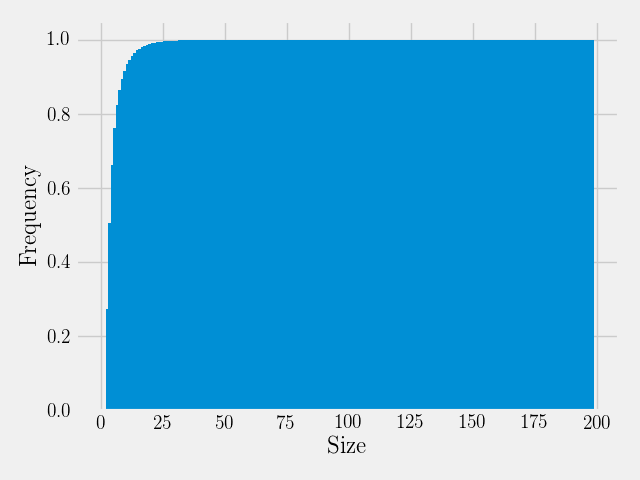
\includegraphics[width=0.3\textwidth]{intersections/total.png}}
\hfill
\subfloat[Largest intersection including smallest iterator\label{fig:intersection-workload-smallest-biggest}]{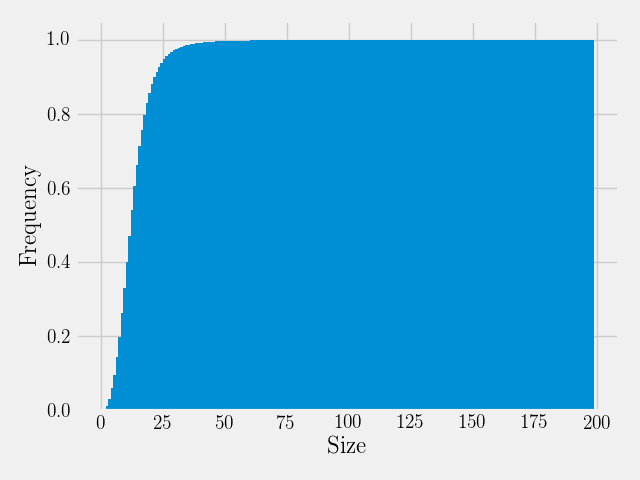
\includegraphics[width=0.3\textwidth]{intersections/smallest-biggest.png}}
\hfill
\subfloat[Smallest iterator\label{fig:intersection-workload-smallest}]{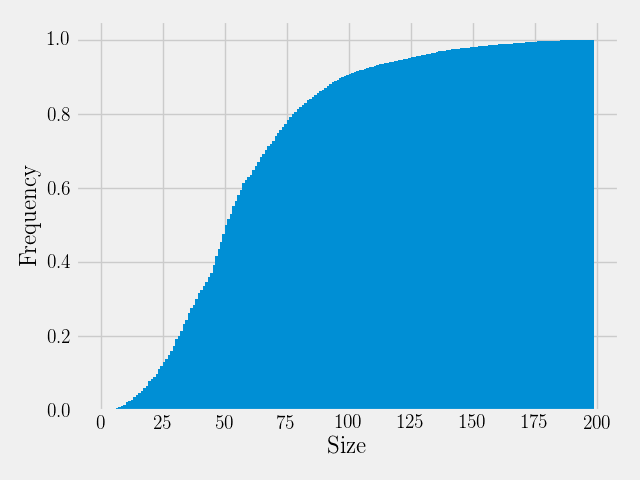
\includegraphics[width=0.3\textwidth]{intersections/smallest.png}}
\caption{Cumulative histograms of total intersection sizes, largest intersection with the smallest iterator and any other, and size of the
smallest iterator participating in \texttt{5-clique} on \texttt{SNB-sf-1}.}
\label{fig:intersection-workload}
\end{figure}

% TODO flowy handover from paragraph to paragraph
In the coming paragraphs, we detail how to build the n-way intersection of multiple adjacency list
such that we gain performance by better use of data-locality than original the \textit{Leapfrog join}.
We choose to use pairwise intersections over multi-way intersection algorithms for their simpler,
linear memory access patterns.

From our analysis, we conclude that the final intersection size is strongly dependent on the
smallest iterator and that the intersection of the smallest iterator with any other iterator is
close to the final size.
These insights translate into two design decisions.
First, we start with the smallest iterator\footnote{We take advantage of the fact that CSR allows us
to determine the size of iterators cheaply (see~\cref{ssec:csr-impl})}.
However, we do not take the sizes of any other iterators into account because the effort for
sorting the iterators by size would not pay off.

Second, we use two different tactics to build the pairwise intersections.
The first intersection between two iterators is built \textit{in-tandem},  where we seek
the upper bound of the higher value in the smaller iterator.
This algorithm guarantees to find the intersection between two iterators in the asymptotical fastest
way.
After this first intersection, the intermediary result is quite small.
Therefore, we use the simpler scheme of linearly iterating the intermediary and probing
the iterator by binary search with fall-back to linear search.

Finally, we point out a few exceptional cases and pitfalls for implementors:
\begin{itemize}
\item If all iterators of the \textit{Leapfrog join} are on their first level, the intersection is near |V|. In this case, we fall back
to the original
\textit{Leapfrog join}.
\item We use an array to materialize the intersections because Scala collections are slow.
Instead of deleting elements, we replace them with a special value.
\item Allocating a new array for every \textit{Leapfrog join} initialization is costly.
We estimate the size of the intersection by the size of the smallest iterator and reuse the array whenever possible. We use a sentry element to mark the end of the array.
\end{itemize}

The carefully chosen operations explained above are faster than the original \textit{Leapfrog join}
algorithm for two reasons.
First, although, the original algorithm uses an asymptotical better n-way intersection, multiple
binary intersections are preferable with the rather small adjacency lists of graph workloads.
In particular, in our situation where the size of the first binary intersection is already
very close to the size of the final intersection.

Second, the \textit{Leapfrog join} generates a single value, then yields control to other parts
of the \textit{LeapfrogTriejoin} algorithm and later touches the same adjacency lists again to generate the next value.
Our approach touches the adjacency lists exactly once per \textit{Leapfrog} initialization and
condenses the intersection into a much smaller array.
This array is more likely to stay cached while the other parts of the \textit{LeapfrogTriejoin} do their work.

\Cref{fig:mat-vs-nomat} shows that a materialized \textit{Leapfrog join} out-performance better than
the original algorithm.
As expected, the optimization is more powerful for bigger queries because they work with more
adjacency lists per \textit{Leapfrog join}, e.g. for a triangle each \textit{Leapfrog join} intersects
only two iterators while for a \texttt{5-clique} each join handles 5 adjacency lists.
Anyhow, even for the triangle query, we see a small but clear improvement and a lower error due to
better cache use.
We refer the reader to our experiment section (\ref{sec:experiments}) for further experiments on
our graph specialized \textsc{wcoj} and detailed descriptions of the datasets and queries used.

\begin{figure}[H]
\centering
% TODO more queries
% TODO add amazon graph
% TODO rename dataset to materialization and no materialization or such
\includesvg{mat-graph-bar-snb-sf1}
\caption{Barchart showing \texttt{GraphWCOJ} with and without \textit{Leapfrog join} materialization
enabled for different queries on \texttt{SNB-sf1}.}
\label{fig:mat-vs-nomat}
\end{figure}
\section{Spark integration}\label{sec:spark-integration}

\subsection{User interface} \label{ssec:user-interface}
\begin{listing}[H]
    \centering
    \inputminted{scala}{code/usage-example.scala}
    \caption{Example usage of a WCOJ to find triangles in graph.}
    \label{lst:usage-example}
\end{listing}

As one can see in line 16 % LINE
of~\cref{lst:usage-example}, we support a clean and precise DSL to match patterns in graphs.
This DSL is inspired by GraphFrames~\cite{graphframe}.
The user can define a pattern by its edges, each edge is written as \textit{(a) - [] -> (b)} where \textit{a} is the
source vertice and \textit{b} is the destination, multiple edges are separated by a semicolon.
A connected pattern is expressed by defining multiple edges with the same source or destination.
One should be aware, that a named source or destination is not guaranteed to be a distinct element in the graph,
e.g. \textit{(a) - [] -> (b); (b) - [] -> (c)} could be a linear path of size two or a circle between \textit{a} and
\textit{b}; in the second case \textit{a} and \textit{c} are the same element.
The reader might wonders, why we chose to stay with the GraphFrame syntax for edges of
\textit{- [] ->}, although, we could have went with something simpler, like \textit{->}.
However, sticking to the more verbose syntax allows us to include labels inside of the squared brackets
in future extensions, e.g. for our stretch goal of integration with CAPS.

The second parameter to \textit{findPattern} allows the user to specify the variable ordering used in the WCOJ algorithm.
Furthermore, the user interface takes multiple optional arguments, e.g. to apply to common filters to the output of the result,
specify different relationships to be used as input for each edge of the pattern.
The filters are \textit{distinctFilter}, ensuring that each vertice can occur only as binding for one variable, and
\textit{smallerThanFilter} to allow only output bindings were the values decrease with regards to the specified variable ordering,
e.g. the binding \textit{[1, 2, 3]} but not \textit{[2, 1, 3]} for the triangle query above.
We experienced that these queries are typical for graph queries and that the performance greatly benefits from pushing
them into the join.
Implementing the possibility to push general filters into the join would be a valuable addition but we decided against it because
it a pure engineering task.

\subsection{Integration with Catalyst} \label{ssec:integration-with-catalyst}
% make clear catalyst ist the only thing we change


We integrated our WCOJ implementation into Spark such that it can be used as function on \textit{Datasets}.
Therefore, we build all components necessary to execute a WCOJ in Spark's structured queries, provided by Catalyst (see
\cref{subsubsec:catalyst}).
First of all this is logical plan representing a worst-case optimal join.
Then a strategy to convert this logical operator into multiple physical operators.
One physical operator executes the join.
In between, this operator and the graph edge relationships, we execute another physical operator that materializes
the graph edge relationships into a data structure that can support a \textit{TrieIterator} interface
(see~\cref{subsubsec:leapfrog-triejoin}).
The integration itself is quite straightforward due to Catalysts extendability.
We explain it in the next sections.
First, we highlight some limitations of our integration into Catalyst.

It is not in the scope of this work to integrate WCOJ's into the SQL parser of Spark.
Hence, WCOJ can only be used by Spark's Scala functional interface and not through Spark's SQL queries.

We do not integrate it into the query optimization components of Catalyst, e.g. we do not provide rules or cost-based strategies to
decide when to use a WCOJ or a binary join.
It is up to the user to decide when to use a WCOJ or a binary join.
However, our integration allows the user to intermix these freely.
The reason for this decision is, that at time of writing no published paper existed that systematically studies which queries benefit from
WCOJ's in general, nor, does research exist that studies the combination of WCOJ's and binary joins.
Only a month after we decided on our scope for Spark integration Salihoglu et al. published an arXiv paper~\cite{mhedhbi2019} that
tackled these problems for the first time.
The lack of peer-reviewed papers and the high complexity of the arXiv paper clearly illustrate that deeper integration with
Spark's optimizer is out of scope for this thesis.


\subsection{A sequetial linear Leapfrog Triejoin} \label{subsec:spark-integration-seq}
For this section we assume that the reader is familiar with the background section about Catalyst (see \cref{subsubsec:catalyst}) and
\textsc{LFTJ} (see \cref{subsubsec:leapfrog-triejoin}) where we explain the components of Catalyst planning phase and the requirements
of a Leapfrog Triejoin.
In the current section, we outline how to satisfy the requirments of \textsc{LFTJ} within and help of Catalysts structured plans.

Our baseline implementation of the Leapfrog Triejoin is a sequential implemenation, i.e. it is not distributed.
Therefore, all representations of the edge relationship have only a single partition which the join operates upon.
In Spark this partitioning is called \textit{AllTuples}.
We enforce sequential execution of the complete Spark plan in our experiments by setting the number of executors to 1.

In the first phases of Catalyst query compilation process, the query plan is represented by logical operators.
Integration into this phase only requires us to build a logical operator to represent the \textsc{WCOJ} join.
A \textsc{LFTJ} can have 2 or more children, one for each input relationship.

The logical and physical plan for the triangle query is shown in~\cref{fig:wcoj-catalyst-plan}.

\begin{figure}
%    \subfloat[Logical plan]{\includesvg[width=0.5\textwidth]{wcoj-catalyst-logical-plan}}
%    \subfloat[Physical plan]{\includesvg[width=0.5\textwidth]{wcoj-catalyst-physical-plan}}
    \caption{Catalyst plans for the triangle query using a Leapfrog Triejoin.}
    \label{fig:wcoj-catalyst-plan}
\end{figure}

The strategy to translate the logical plan into a physical plan has to tasks.
First, simply translating the n-ary logical plan into n-ary physical plan that executes the \textsc{LFTJ} with the children as input.
Second, introducing a physical operator per child which materializes the RDD into a sorted, columnar array representation to support a
\textit{TrieIterator} interface.

The first physical operator is straightforward to implement.
It simply executes a \textit{LFTJ} over the \textit{TrieIterators} provided by the children.
Given that each child has only one partition and there are no parallel operations, the algorithm can be implemented exactly
as described in~\cref{subsubsec:leapfrog-triejoin}.

The second physical operator translates the linear interator interface of any RDD into a \textit{TrieIterator} interface.
In particular, it needs to offer a \textit{seek} operation in $\mathcal{O} (\log N) $.
To support this interface the operator requires its children to be sorted;
this requirement can be fulfilled by Catalyst standard optimization rules.
Then it takes the sorted linear iterator and materializes it into a column-wise array structure.
Given this data structure, the \textit{TrieIterator} can be implemented using binary search (as described
in~\cref{subsubsec:leapfrog-triejoin}).

\subsection{GraphWCOJ} \label{subsec:spark-integration-graphWCOJ}
% TODO maybe i miss a good connection between variable ordering and sorting and the fact that I need only two tables?
The integration of GraphWCOJ is quite similar to the one of \textsc{LFTJ}.
\Cref{fig:graphWCOJ-catalyst-plan} shows the logical and physical plan constructred by our integration.
There are three main difference: GraphWCOJ requires only two children for the input relationships, the children materialize the input
relationships in a CSR data structure (see~\cref{subsec:csr-background}) and we support parallel execution of the join (which requires
a third child) and broadcasting the CSR data structure.
We address these differences in order.

Our GraphWCOJ operators need only two materialized version of the input relationship.
This is because in graph pattern matching the joins are self-joins on the edge relationship.
The \textsc{LFTJ} requires that its input relationships are sorted by an lexicographic sorting over the variable ordering.
To support all possible variable orderings, we need the edge relationship sorted by $src, dst$ and $dst, src$.
Hence, we need to separate, materialized versions of the edge relationship.

GraphWCOJ uses a CSR representation of the edge relationship (see~\cref{sec:graphwcoj}).
% TODO CSR accessible and sorted? definition not given.
Hence, we need to build two CSR representations.
One with its \textit{Indices} array build from the $src$ attribute and the \textit{AdjancencyLists} array build from the $dst$ attribute.
The other, with \textit{Indices} from $dst$ and \textit{AdjacencyLists} from $src$.
Next, we describe how to build these CSR's from two linear, sorted, row wise iterators as provided by Spark for the two child relationships.

% TODO algorithm to build them
First, we note that it is necessary to build both compressed sparse row data structures in tandem.
This is because some vertices in the graph might have no outgoing or incoming edges.
That means some vertice ID's do not occur in the $src$ or $dst$ attributes of any tuple.
Therefore, the \textit{Indices} arrays of the two CSR structures would differ if they are build from either $src$ and $dst$, e.g.
they could have different length.
However, if this is the case, it is not possible to use both CSR's together in a single join.

To allow building the CSR's in-tandem, we introduce \textit{AlignedZippedIterator}.
The \textit{next} method of this iterator is shown in~\cref{alg:alignedZippedIterator}.
It zips two iterators of two-tuple elements and aligns them on the first component, e.g. edges with $src$ as first component and $dst$ as
second component.
The zipped iterator emits triples where the first component is the aligned first element of both underlying iterators and the other
two elements are the second components of both iterators.
If the two iterators have different numbers of elements with the same first component, we advance only one iterator and fill the missing
component in the emitted triple with a placeholder until the first component of both iterators aligns again.

\begin{algorithm}
  \uIf{iter1.hasNext() and iter2.hasNext()} {
    t1 $\leftarrow$ iter1.peek() \;
    t2 $\leftarrow$ iter2.peek() \;
    \uIf {t1[0] == t2[0]} {
      iter1.next()\;
      iter2.next()\;
      \KwRet{(iter1.key()[0], iter1.key()[1], iter2.key()[1])}\;
    } \uElseIf{t1[0] < t2[0]} {
      iter1.next()\;
      \KwRet{(iter1.key()[0], iter1.key()[1], -1)} \;
    } \Else {
      iter2.next()\;
      \KwRet{(iter2.key()[0], -1, iter2.key()[1])} \;
    }
  } \uElseIf {iter1.hasNext()} {
    iter1.next() \;
    \KwRet{(iter1.key()[0], iter1.key()[1], -1)} \;
  } \Else {
    iter2.next() \;
    \KwRet{(iter2.key()[0], -1, iter2.key()[1])} \;
  }
  \caption{\textit{next} method of an \textit{AlignedZippedIterator}.}
  \label{alg:alignedZippedIterator}
\end{algorithm}

Given an \textit{AlignedZippedIterator} over both input relationships, it is straightforward to build both CSR data structures.
We consume the whole \textit{AlignedZippedIterator}, for each element we append the 2nd and 3rd component to \textit{AdjacencyLists} of
the CSR's;
while skipping placeholders.
Whenever the first element of the three tuple changes, we append the current size of the \textit{AdjaencyLists} buffers to the
\textit{Idices} arrays.

The final difference between the Spark integration for \textsc{LFTJ} and GraphWCOJ is that we build GraphWCOJ such that it can
be run in parallel.

As argued in former chapters, we broadcast the edge relationship to all workers.
The broadcast is supported by Spark's broadcast variables (see~\cref{subsubsec:broadcast-variables}) and Catalysts support to broadcast
the execution of a physical operator.

Parallelism is introduced via the third child of our GraphWCOJ operators.
It is an empty RDD with as many partitions as the desired level of parallelism.
We schedule tasks by using the \textit{mapPartitions} function of this empty RDD.
Foreach partition, we run the \textsc{WCOJ} join backing its \textit{TrieIterator} with the broadcasted CSR's and partition the data
logical by one of the schemes described in~\cref{sec:worst-case-optimal-join-parallelization}.


% Broadcast cache
One of the main advantages of broadcasting the edge relationship to all workers is that we can reuse the same broadcast for all queries
over the same graph.
To support this in Catalyst, we introduce one additional physical operator which we call \textit{ReusedCSRBroadcast} and a CSR broadcast
variable cache maintained on the Spark master node.

The CSR broadcast variable cache is a simple dictionary with RDD ID's to broadcast variables of CSR structures.
When, our system builds a broadcasted CSR structure, it registers the broadcast in the cache.
Everytime, we translate a logical WCOJ plan into a physical one, we check if the CSR for edge relationship has been broadcasted already
if so, our strategy reuses this broadcast.


% TODO disk cache?
% CSR disk cache  % CSRTrieIterableBroadcast implements that

% connection to distribution, logical partitionings integrated into the GraphWCOJ algorithm


% TODO where whole system overview as one big diagram, and then used to explain the structure? introduction, extra chapter after background.

% TODO move to acknowledgements
The Spark integration of this work has been inspired by the IndexedDataframes~\cite{indexed-dataframes} work of Alex Uta and the supervisors
of this thesis.



\section{Experiments}\label{sec:experiments}

TODO introduction

\subsection{Setup}

We run our experiments on machines of the type \texttt{diamond} of the Scilens cluster owned by the CWI Database Architecture research
group.
These machines feature 4 Intel Xeon E5-4657Lv2 processors with 12 cores each and hyperthreading of 2 (48 cores / 96 threads)
Each core has 32 KB of 1st level cache, 32KB 2nd level cache.
The 3rd level cache are 30 MB shared between 12 cores.
The main memory consists of 1 TB of RAM DDR-3 memory.

The machines run a Fedora version 30 Linux system with the 5.0.17-300.fc30.x86\_64 kernel.
We use Spark 2.4.0 with Scala 2.11.12 on Java openJDK 1.8.
In the majority of our experiments, we use Spark in its standard configuration with enabled code generation.
We also tune the parameters for driver and executor memory usage (\texttt{spark.driver.memory} and \texttt{spark.executor.memory}) to fit
all necessary data into main memory.

\subsubsection{Algorithms}

In our experiments we use 4 different join algorithms.
Two of them are worst-case optimal joins.
That is our Leapfrog Triejoin implementation and a graph-pattern matching
specialized Leapfrog Triejoin developed in this thesis: Graph\textsc{WCOJ}.
LFTJ is only run as sequential algorithm as a baseline against GraphWCOJ.
We compare these two algorithms in \cref{subsec:lftj-vs-graphWCOJ}.

The other two algorithms are Spark's binary joins: \textit{BroadcastHashJoin} and \textit{SortmergeJoin}.
We compare them against the sequential version of \textsc{LFTJ} and GraphWCOJ in \cref{subsec:seq-vs-spark}.

We adjust the \texttt{"spark.sql.autoBroadcastJoinThreshold"} parameter to control
if Spark is using a \textit{BroadcastHashJoin} or a \textit{SortMergeJoin}.

\subsubsection{Datasets}
We run the our experiments on multiple datasets from two different use-cases: social networks and product co-purchase.
We motivate our choice in the next paragraph.
\Cref{table:datasets} includes a list of all graph datasets mentioned throughout the thesis.

\begin{table}[]
    \centering
    \begin{tabular}{llrrl} \toprule
        Name    & Variant              &  Vertices   & Edges          & Source          \\ \midrule
        \textbf{SNB}         & sf1     &             &  453.032       & \cite{snb}      \\
        \textbf{Amazon}      & 0302    & 262,111     &  1,234,877     & \cite{snapnets} \\
                             & 0601    & 403,394     &  3,387,388     & \cite{snapnets} \\
        \textbf{Twitter}     & sc-d    & 81,306      &  1,768,135     & \cite{snapnets} \\
%                             & sc-u    &   TODO      &       TODO     & \cite{snapnets} \\
        \textbf{LiveJournal} &         & 4,847,571   & 68,993,773     & \cite{snapnets} \\
        \textbf{Orkut}       &         & 3,072,441   & 117,185,083    & \cite{snapnets} \\ \bottomrule
    \end{tabular}
    \caption{A summary of all datasets mentioned in the thesis.}
    \label{table:datasets}
\end{table}

The SNB benchmark~\cite{snb} generates data emulating the posts, messages and friendships in a social network.
For our experiments, we only use the friendships relationship (\texttt{person\_knows\_person.csv}) which is an undirected relationship.
Only edges of the kind \textit{src $<$ dst} exist, we generate the opposing edges before loading the dataset, such
that the edge table becomes truly undirected.

The benchmark comes with an extensively parameterizable graph generation engine
which allows us to experiment with sizes as small as 1GB and up to 1TB for big experiments and different levels of selectivity.
The different sizes are called scale-factor or \texttt{sf}, e.g. \texttt{SNB-sf1} refers to a Social network benchmark dataset generated with
default parameters and scale-factor 1.

The Amazon co-purchasing network contains edges between products that have been purchased together and hence are closely related to each other~\cite{snapnets}.
This is a directed relationship from the product purchased first to the product purchased second, both directions of an edge can exist if the order in which
products have been purchased varies.

The Snap dataset collection contains multiple Amazon co-purchase datasets, each of them containing a single day of purchases.
We choose the smallest and biggest dataset from the 2nd of March and the 1st of June 2003 which we call them \texttt{Amazon-0302} and
\texttt{Amazon-0601}.

We pick co-purchase datasets for evaluation because former work often concentrated on social networks and web crawl based
graphs~\cite{myria-detailed,ammar2018distributed} but~\cite{salihoglu2018} points out that the biggest graphs are actually graphs like
the aforementioned Amazon graph containing purchase information.

To allow comparisons with former work, we run a subset of our experiments on the Twitter social circle network from~\cite{snapnets}.
This dataset includes the follower relationship of one thousand Twitter users; each of these follows 10 to 4.964 other users and
relationships between these are included.

The \texttt{LiveJournal} graph represents the friendship relationship of a medium sized social network.

\subsubsection{Graph patterns}

In this section, we detail the graph patterns used throughout our experiments.
Most of the queries are cyclic because that has been shown to be the primary use-case for WCOJ in former research~\cite{olddog,myria-detailed}.
WCOJ's also have been successfully applied to selective path queries in~\cite{olddog,longbin}.

We apply filters to most of our queries to make them more realistic, e.g. a clique query does make more sense if it is combined with a
smaller-than filter, which requires that the attributes are bound such that \textit{a} smaller than \textit{b}, smaller than \textit{c}.
Otherwise, one gets the same clique in all possible orders, which not only takes much more time but is also most
likely not the result a user would want.

We ensure that filters can be pushed down through or in the join by Spark as well as by the WCOJ to compare both algorithms on an equal basis.
A complete list of all queries and filters used is shown in~\cref{table:patterns}.
\Cref{fig:all-queries} shows depiction of all graph patterns.

Patterns and filters are combined as follows.
Cliques and the \texttt{kite} query use smaller than filters which require the bindings to increase
in value according to the variable ordering.
All other queries are run with a filter such that each of their binding must be distinct.

\begin{table}[]
    \centering
    \begin{tabular}{@{}lcccp{6cm}@{}}
        \toprule
        Name     & Parameters                 & Vertices & Edges

        \\ \midrule
        \texttt{triangle} & NA                          & $3$        & 3                 \\
        \texttt{n-clique} & \# vertices                & $n$        & $1/2 \times n \times (n - 1)$ \\
        \texttt{n-cycle}  & \# vertices                & $n$        & $n$                 \\
        \texttt{n-s-path} & \# edges / selectivity  & $n$       & $n - 1$                 \\
    \texttt{kite}  & NA                         & $4$        & $5$                    \\
        \texttt{house}    & NA                         & $5$        & $9$                 \\
        \texttt{diamond}  & NA                         & $4$        & $4$                 \\
        \textbf{Filters}   &                            &          &                   \\
        \texttt{distinct}  &                            &          &                   \\
        \texttt{less-than} &                            &          &                   \\ \bottomrule
    \end{tabular}
    \caption{Summary of patterns and filters used.}
    \label{table:patterns}
\end{table}

\begin{figure}
    \centering
    \subfloat[triangle]{\includesvg[width=0.2\textwidth]{svg/triangle}}
    \subfloat[4-clique]{\includesvg[width=0.2\textwidth]{svg/4clique}}
    \subfloat[5-clique]{\includesvg[width=0.2\textwidth]{svg/5clique}}
    \subfloat[4-cycle]{\includesvg[width=0.2\textwidth]{svg/4cycle}}\\
    \subfloat[5-cycle]{\includesvg[width=0.2\textwidth]{svg/5cycle}}
    \subfloat[diamond]{\includesvg[width=0.2\textwidth]{svg/diamond}}
    \subfloat[kite]{\includesvg[width=0.2\textwidth]{svg/kite}}
    \caption{Queries used in our experiments.}
    \label{fig:all-queries}
\end{figure}

For a selective path query, we first select two sets of nodes with respect to the \textit{selectivity} parameter.
Then we search for all paths of a certain length according to the \textit{edges} parameter, e.g. \texttt{4-0.1-path} finds all
paths between two randomly selected, fixed sets of vertices of length 4.
The sets of nodes contain roughly 10\% of all input nodes and are
not guaranteed to be intersection free.

\subsection{Linear search threshold}\label{subsec:linear-search-threshold}

We run \textsc{LFTJ} and GraphWCOJ with different settings for the \textit{linear search threshold}.
As explained in \cref{subsubsec:leapfrog-triejoin}, we use a binary search to implement the \textit{seek}
method of the \textit{TrieIterators};
it is also used for GraphWCOJ.
It is well known, that a binary search can be optimized by ending it with a linear search on small
search spaces because linear memory access patterns are cheaper than random accesses.
The threshold gives the size of the search space from which to use a linear search instead of
a binary search, e.g. a threshold of 40 means that the algorithm switches to a linear search
once the search space is 40 numbers or less.

We note that \textsc{LFTJ} and GraphWCOJ could behave differently for the same threshold.
This is because Leapfrog Triejoin uses a binary search for both levels of its \textit{TrieIterators},
while GraphWCOJ only uses the binary search for the second levels;
the first level is indexed in a \textsc{CSR}.

In this experiment, we vary the threshold between 1 and 1600 to determine the best value.
These values are chosen such that 1 does not trigger any linear search and that 1600
does not improve the performance anymore (for \textsc{LFTJ}) and triggers no
binary search for GraphWCOJ.
We do so for the 5-clique query on the SNB-1 and on the Twitter dataset.

The results are shown in \cref{fig:linear-search-threshold-snb} and~\ref{fig:linear-search-threshold-twitter}.
The optimum for LFTJ is around 200 while GraphWCOJ shows the best performance at 1600 and 800 for
SNB-1 respectively Twitter.
This means that GraphWCOJ performs best when there are nearly no binary searches.
A threshold of 1600 triggers no binary search in either of the datasets.

We also note that the effect on the performance of the Leapfrog Triejoin is bigger.

\begin{figure}
    \centering
    \subfloat[SNB-1\label{fig:linear-search-threshold-snb}]{\includesvg[width=0.5\textwidth]{svg/linear-search-threshold-snb}}
    \subfloat[Twitter\label{fig:linear-search-threshold-twitter}]{\includesvg[width=0.5\textwidth]{svg/linear-search-threshold-twitter}}
    \caption{Runtime of \textsc{WCOJs} with different settings for the linear search thresholds.}
\end{figure}

We explain the observations as follows: \textsc{LFTJ} does use searches on the first
and second level of the \textit{TrieIterators} while GraphWCOJ uses it only on the second
level.
Hence, the impact is bigger.

The optimal values are different because data of the levels is differently distributed.
The first level lists nearly all vertices while the second level is made of adjacency lists which are more
sparse.
Hence, we assume that the linear searches on the first level are generally longer than
the one on the second level;
note that the threshold only gives an maximum length for linear searches but this is not
necessarily a good indicator for the length of the performed search.

We tried to use different threshold values for the two levels in \textsc{LFTJ}.
We choose the values 200 for the first level and 1600 for the second level because these
are the optimal values according to our experiments.
However, we note that no huge performance gain can be measured.
This is most likely because the runtime is dominated by the searches on the first level.
For simplicity, we do not use two different thresholds for \textsc{LFTJ} in any further experiments.

From this experiment, we conclude that the optimal threshold for \textsc{LFTJ} is 200 and 800
for GraphWCOJ.
We choose 800 for GraphWCOJ because it is on the safe site:
a binary search performance degrades less than the one of a linear search.
We set these values accordingly in the all further experiments.


\subsection{Baseline: \texttt{BroadcastHashJoin} vs \texttt{seq}}
% TODO use uniform spelling for broadcasthashjoin
In this experiment, we compare the runtime of our sequential Leapfrog Triejoin implementation with the runtime of Spark's \texttt{BroadcastHashjoin}.
Towards, this goal we ran all queries from~\cref{table:patterns} on our three of our datasets: \texttt{Amazon-0302}, \texttt{Amazon-0601}
and
\texttt{SNB-sf1}.


We show our results in~\cref{fig:spark-vs-lftj}.
\Cref{sssec:seq-analysis} analyzes the results.

Our experiment measures the time it takes to perform a \texttt{count} on the cached dataset using \texttt{BroadcastHashjoin} and
\textsc{LFTJ}.
For \texttt{BroadcastHashjoin}, the time to run the whole query is reported.
For \texttt{seq}, we report setup time and the time, it takes to run the join, separately.
Setup time includes the sorting and materialization.
This section is focused on comparing the runtimes excluding the setup time - rational given in~\cref{sssec:seq-experiment-rational}.

\subsubsection{Experiment Setup}\label{sssec:seq-experiment-rational}
\textbf{Question:} Why do we compare against Spark's \texttt{BroadcastHashjoin} instead of \texttt{SortMergeJoin}? \\
\textbf{Answer:} Because even when all data is arranged in a single partition, for simple sequential processing, Spark
schedules its \texttt{SortMergeJoin} to use a shuffle.
A shuffle writes and reads data to and from disk.
Hence, \texttt{SortMergeJoin} is much slower than a \texttt{BroadcastHashJoin}.
We compared the algorithms on the \texttt{Amazon-0601} dataset for the \texttt{triangle} (8.1 seconds vs 58.9 seconds) and
\texttt{5-clique} pattern (32.9 seconds vs 850.9 seconds).
We assume that Spark is able to optimize its broadcasts when \texttt{local[1]} is used to start the Spark session because then Spark uses the driver as executor.

\textbf{Question:} Why do we exclude setup times from the WCOJ times?\\
\textbf{Answer:} Because system is meant to cache the readily sorted and formatted as \textsc{CSR}'s and reuse it for multiple queries.
We anticipate that this is necessary to benefit from \textsc{WCOJ}'s in general.

%\textbf{Question:} Why is the time to copy results into \texttt{UnsafeInternalRow} format for WCOJ counted as setup time?\\
%\textbf{Answer:} It is time solely spent for integration with Spark and not Leapfrog Triejoin specific.
%Furthermore, it could be avoided by working directly on the \texttt{UnsafeInternalRow} format within our \texttt{seq} implementation.
%However, this would require us to work with unmanaged memory (the \texttt{UnsafeInternalRow} interface is slower than working on \texttt{Arrays})
%and we deem this as an unnecessary engineering overhead.

\textbf{Question:} Is Spark's code generation a huge advantage for the \texttt{BroadcastHashjoin}?\\
\textbf{Answer:} Yes, we ran Spark without code generation for comparision on the \texttt{Amazon-0302} dataset for the \texttt{triangle}
query and \texttt{5-clique}: with code generation Spark takes 3.1 and 4.2 seconds without 14 and 16 seconds.

\subsubsection{Analysis}\label{sssec:seq-analysis}

We are able to beat Spark's \texttt{BroadcastHashjoin} on all datasets and queries except \texttt{5-clique-lt} on \texttt{Amazon-0602}.
Generally, we see that for \texttt{n-clique} patterns the speedup over Spark decreases for bigger $n$.
This is due to the fact that many binary joins in a \texttt{n-clique} are actually semi-joins which to do not increase but decrease the size of intermediary results,
e.g. for \texttt{5-clique} on \texttt{Amazon-0302} only 3 out of 9 joins lead to a bigger intermediary result.

The cycle query results are highly interesting because we see an increasing speedup for higher $n$ on \texttt{Amazon-0602} but a
decreasing speedup on \texttt{Amazon-0302}.
% TODO n-cycle results for snb

The \texttt{House} and \texttt{5-clique} pattern seem to be quite similiar - the \texttt{House} is a \texttt{5-clique} with two missing
edges.
However, as the count of their results indicates these two edges lead to dramatically different outcomes.
Hence, their different timing and speedup behaviour.

The \texttt{Kite} pattern produces consistently the second highest speedup after the \texttt{3-clique}.
Most likely due to the fact that a \texttt{Kite} is two triangles back-to-back.

The path query shows very different behaviour on the \texttt{Amazon} and the \texttt{SNB} datasets.
This might be due to the different selectivity; it is extremely high on the co-purchase datasets and rather low on the social network
benchmark.
This different in selectivity is not surprising given that the \texttt{SNB} network fulfills the small world property, while the
\texttt{Amazon} dataset relates products purchased together which naturally leads to multiple loosely connected, denser components.

% TODO maybe run path query with different selectivity

Finally, we observe that all three datasets lead to quite different results which are most likely not comparable to each other without deeper research
in the characteristics of the datasets themselves.

In particular, it becomes clear that co-purchase datasets and social network datasets must have very different characteristics.
Although, \texttt{SNB-sf1} is much smaller than \texttt{Amazon-0601}, queries on it take a similar or even much more time,
e.g. \texttt{5-clique} takes 14.21 seconds on the bigger dataset and 12.65 seconds smaller, even though, the result set is much
smaller on \texttt{SNB-sf1};
\texttt{4-cycles} takes roughly 8 times longer on the small dataset and has a much bigger result set.
In general, we see a higher speedup on \texttt{SNB-sf1}

\begin{figure}
    \centering
    \subfloat[Amazon0302]{
        \includesvg[width=0.5\textwidth]{svg/spark-wcoj-amazon}
        \includesvg[width=0.5\textwidth]{svg/spark-wcoj-amazon-long}
    }\\
    \subfloat[Amazon0601]{
        \includesvg[width=0.5\textwidth]{svg/spark-wcoj-amazon0601}
        \includesvg[width=0.5\textwidth]{svg/spark-wcoj-amazon0601-long}
    }\\
    \subfloat[SNB-sf-1]{
        \includesvg[width=0.5\textwidth]{svg/spark-wcoj-snb}
        \includesvg[width=0.5\textwidth]{svg/spark-wcoj-snb-long}
    }
    \caption{Runtime of a Leapfrog Triejoin and Spark's \texttt{BroadcastHashJoin}}
    \label{fig:spark-vs-lftj}
\end{figure}


%\begin{table}
%    \centering
%
%    \begin{tabular}{lr||r|rr||r}
\toprule
        Query &  \# Result & \texttt{BroadcastHashJoin} & \texttt{seq} & setup & Speedup \\
\midrule
    Clique(3) &    188,705 &                       3.08 &         0.49 &  2.51 &     6.3 \\
    Clique(4) &     47,824 &                       3.85 &         1.25 &  4.55 &     3.1 \\
    Clique(5) &      7,064 &                       4.22 &         2.32 &  7.60 &     1.8 \\
        House &  2,941,664 &                       7.87 &         5.66 &  6.18 &     1.4 \\
         Kite &    220,637 &                       3.82 &         1.04 &  6.73 &     3.7 \\
     Cycle(4) &  3,076,324 &                       4.90 &         2.75 &  3.40 &     1.8 \\
     Cycle(5) &  6,389,425 &                      13.15 &         8.28 &  4.87 &     1.6 \\
     Cycle(6) & 11,682,732 &                      38.00 &        27.62 &  6.79 &     1.4 \\
 Path-3-0.001 &      2,092 &                       1.36 &         0.01 &  0.89 &   136.0 \\
 Path-4-0.001 &      8,829 &                       3.11 &         0.03 &  1.58 &   103.7 \\
\bottomrule
\end{tabular}

%    \vspace{0.3cm}
%
%    \begin{tabular}{lr||r|rr||r}
\toprule
        Query &     \# Result & \texttt{BroadcastHashJoin} & \texttt{seq} &  setup & Speedup \\
\midrule
    Clique(3) &     1,137,579 &                       9.25 &         1.92 &   6.23 &     4.8 \\
    Clique(4) &       911,548 &                      13.97 &         7.12 &  11.74 &     2.0 \\
    Clique(5) &       585,171 &                      12.27 &        14.21 &  19.23 &     0.9 \\
        House &   177,745,510 &                      66.53 &        57.37 &  23.45 &     1.2 \\
         Kite &     3,672,375 &                      13.67 &         5.40 &  15.93 &     2.5 \\
     Cycle(4) &    45,175,984 &                      37.76 &        21.77 &  14.12 &     1.7 \\
     Cycle(5) &   263,436,965 &                     227.97 &       115.60 &  24.96 &     2.0 \\
     Cycle(6) & 1,484,438,088 &                    2020.04 &       872.62 &  83.12 &     2.3 \\
 Path-3-0.001 &        98,929 &                       2.31 &         0.07 &   2.30 &    33.0 \\
 Path-4-0.001 &       922,888 &                       5.61 &         0.52 &   4.25 &    10.8 \\
\bottomrule
\end{tabular}

%
%    \vspace{0.3cm}
%    \begin{tabular}{lr||r|rr||r}
\toprule
        Query &     \# Result & \texttt{BroadcastHashJoin} & \texttt{seq} &   setup & Speedup \\
\midrule
    Clique(3) &       540,225 &                      11.88 &         0.73 &    1.09 &    16.3 \\
    Clique(4) &       260,786 &                      15.43 &         4.85 &    2.33 &     3.2 \\
    Clique(5) &        40,137 &                      18.64 &        12.65 &    3.08 &     1.5 \\
        House &   100,206,468 &                     300.13 &        85.18 &    6.58 &     3.5 \\
         Kite &     1,780,235 &                      21.59 &         2.45 &    2.20 &     8.8 \\
     Cycle(4) &   232,636,376 &                     636.77 &       162.89 &   10.68 &     3.9 \\
 Path-3-0.001 &    65,290,479 &                       1.76 &         6.05 &    3.28 &     0.3 \\
 Path-4-0.001 & 7,235,522,926 &                     111.73 &       655.52 &  293.27 &     0.2 \\
\bottomrule
\end{tabular}

%    \caption{Runtimes for \texttt{BroadcastHashJoin} and \texttt{seq}.
%    The speedup is calculated between join times and excludes setup.
%    From top to bottom for dataset: \texttt{ama-0302}, \texttt{ama-0601} and \texttt{snb-sf1}.
%    All times in seconds.
%    }
%    \label{table:seq-vs-bhj}
%    % TODO align and remove headers
%\end{table}

\subsection{\textsc{LFTJ} vs GraphWCOJ} \label{subsec:lftj-vs-graphWCOJ}

In this experiment, we compare sequentials runs of the Leapfrog Triejoin and GraphWCOJ
on the \texttt{Amazon}, \texttt{SNB-1} and \texttt{Twitter} datasets.
We do not show the run-time of \texttt{Path} queries because GraphWCOJ is not able to run
them\footnote{\texttt{Path} queries require us to filter the input relationship before
the join. This has not been implemented for GraphWCOJ due to time constraints.}.

We show the results for the different datasets in~\cref{fig:lftj-graphWCOJ}.


\begin{figure}
    \subfloat[Amazon-0302]{\includesvg[width=0.3\textwidth]{svg/lftj-graphWCOJ-amazon}}
    \subfloat[Amazon-0601]{
      \includesvg[width=0.3\textwidth]{svg/lftj-graphWCOJ-amazon0601}
      \includesvg[width=0.3\textwidth]{svg/lftj-graphWCOJ-amazon0601-long}
    }\\
    \subfloat[SNB-1]{
    \includesvg[width=0.3\textwidth]{svg/lftj-graphWCOJ-snb}
    \includesvg[width=0.3\textwidth]{svg/lftj-graphWCOJ-snb-long}
    }\\
    \subfloat[Twitter]{
    \includesvg[width=0.3\textwidth]{svg/lftj-graphWCOJ-twitter}
%    \includesvg[width=0.3\textwidth]{svg/lftj-graphWCOJ-twitter-long}
    }
    \caption{WCOJ run time of \textsc{LFTJ} and GraphWCOJ on different datasets and queries.}
    \label{fig:lftj-graphWCOJ}
\end{figure}

\subsection{Scaling of \textit{Graph\textsc{WCOJ}}} \label{subsec:scaling-graphWCOJ}

In this section, we aim to analyse and compare the scaling of Graph\textsc{WCOJ} using different
partitioning schemes.
Towards this goal, we run Graph\textsc{WCOJ} on datasets of different size namely \texttt{Twitter},
\texttt{LiveJournal} and \texttt{Orkut}.
We compare two partitioning schemes: Shares and work-stealing.
These are the two most promising schemed identified in \cref{sec:worst-case-optimal-join-parallelization}.
The experiment is performed on 3-clique and 5-clique.
3-clique is the smallest of our queries.
Therefore, it is most difficult to scale.
5-clique takes much longer than 3-clique.
Hence, it shows how query size influences the scaling.
Also, it increases the job size for the \textit{work-stealing} partitioning scheme.

% TODO paragraph about section structure

\subsubsection{Results}

\begin{figure}
    \centering
    \subfloat[Twitter dataset\label{fig:graphWCOJ-scaling-twitter}]
      {\includesvg[width=0.5\textwidth]{svg/graphWCOJ-scaling-twitter}}
    \subfloat[LiveJournal dataset\label{fig:graphWCOJ-scaling-livej}]
      {\includesvg[width=0.5\textwidth]{svg/graphWCOJ-scaling-livej}}
    \newline
    \subfloat[Orkut dataset\label{fig:graphWCOJ-scaling-orkut}]
      {\includesvg[width=0.5\textwidth]{svg/graphWCOJ-scaling-orkut}}
    \caption{Scaling behaviour of Shares and work-stealing on three different datasets
      and two different queries.
      The batch size parameter for \textit{work-stealing} is chosen for balance between lock contention and worker skew:
      50 for Twitter and 3-clique on LiveJournal, 1 for 5-clique on LiveJournal and 20 on the Orkut dataset.
    }
    \label{fig:graphWCOJ-scaling}
\end{figure}

We first describe our expectations of the experiment outcome.
We assume that scaling improves with the dataset size.
Hence, we should see the highest speedups for Orkut, then LiveJournal and the lowest speedups for Twitter.
Also, we expect the scaling to improve with the query size.
Both hypothesis are grounded in the fact that more work to distribute often leads to stronger scaling.
Additionally, we believe that \textit{work-stealing} shows better scaling than Shares because it does not duplicate work.
Finally, we have no clear cut expectations to the scaling behaviour of \textit{work-stealing}.
Theoretically, we could expect linear scaling for it because no work is duplicated, synchronization overhead is minimal and
work balance should be given by the scheme.
However, we measure on a quite complex hardware platform which complicates scaling behaviour.

First of all, we work on a machine with 4 sockets.
This can influence scaling positively and negatively.
Positively because adding more sockets means to add significantly more L3 cache (30 MB shared per socket).
If we do not use all cores on a socket, each used core can use a bigger share of this cache.
Negatively because each socket is in a different NUMA zone and the graph is not guarantued to be chached in all
NUMA zone.
Indeed, Spark shares the broadcasts for all tasks on a single executor.
So there is only one copy in memory.

Additionally, we run on an Intel processor with hyperthreading.
Hence, we can not expect linear speedup above 48 workers because after multiple threads will share resources and cannot be
expected to reach the same performance as two cores.

To conclude, we expect sub-linear speedup for Shares and better but still sub-linear speedup for \textit{work-stealing}.
Anyhow, it super-linear scaling in MapReduce like systems is not unheard of and could be possible on our machines.
% TODO cite the internet source from Monday.

We describe our observations per dataset;
starting with Twitter.
As expected, both partitioning schemes scale better when we increase the query size.
For 5-clique, \textit{work-stealing} exhibits near linear scaling up to 48 workers, while
clique-3 reaches the maximum speedup of 6.22 for 8 workers.
The highest speedup for 5-clique is 45 on 96 workers; clique-3 reaches its highest speedup
with 13.2 on 64 workers.
Shares lacks behind in scaling for both queries and all levels of parallelism.
The best observed speedup is 21.3 for 5-clique and 96 workers.
% TODO spark overhead
% TODO bad scaling for hyperthreading

The experiment on LiveJournal confirms our hypothesis that bigger datasets lead to better
speedups;
the highest observed speedup is 61.2 for \textit{work-stealing} on 3-clique and
36.81 for Shares on 5-clique each with 96 workers.
Also, we can confirm that Shares scales better on 5-clique than on 3-clique; with the exception of 32 workers.
However, this is not the case for \textit{work-stealing}.
\textit{work-stealing} shows better speedups on clique-3 than on clique-5.
Nevertheless, \textit{work-stealing} beats Shares on both queries and all levels of parallelism.
% TODO analyse, higher skew rigth, at least name reason, is skew higher because of 0th vertice?
% TODO effect of dataset size leads to 5-clique scaling the same or worse

Additionally, we see two strange scaling behaviours for LiveJournal.
First, super-linear scaling for 3-clique and \textit{work-stealing}.
We hypnotize that this is the fact because if the 32 processes are distributed over all 4 sockets they share in total
120 MB of L3 cache while a single process can use only 30 MB of L3 cache.
%To confirm this we rerun the experiment with 1, 8, 16 and 32 workers while using \textit{taskset} to bind the application
%to the first 8, 16 or 32 cores.
%This rules out the use of more than 1, 2 or 3 sockets respectively.
%In this experiment, we measure speedup of 8.6, 16.6 and 32.9 for 8, 16 and 32 workers.
%This is significantly lower than the speedup measurements without \textit{taskset}.
%We conclude that this confirms our hypothesis and believe that the slight super-linear
%scaling that remains arises from the bigger amount of L1 and L2 cache in the system.
% TODO run with perf counter
% TODO note why do we have locallity in data accesses?

Second, Shares exhibits lower speedup of 12.1 for 64 workers which is
lower than for 32 workers (14.7) and 14.8 for 96 workers.
This can be explained by the chosen Shares configuration.
For 32 workers, the best configuration is given by the hypercube of the sizes 4, 4, 2.
For 64 workers, we get the hypercube with 4 workers on each axis.
Hence, although we are doubling the number of workers, we use the new workers only to partition
work along the last axis, in the case of 3-clique along the C attribute axis.
Partitioning work along the last axis leads to a high amount of duplicated work on the first
two axis.
Additionally, with 64 workers at least 12 of these workers are not exclusive cores but cores shared by
two hyperthreads.
In total, we get a lower speedup.
This changes slightly for 96 workers because the optimal hypercube configuration here is 6, 4, 4 which
adds more workers along the first axis.
However, the scaling only increases marginally by 0.1 from 32 workers which is quite disappointing given
that the number of threads increased by a threefold.

One could argue that we should use a different definition of \textit{best} hypercube configuration.
As we see, it is not necessarily efficient to distribute the computation along the last axis.
% TODO prefix shares
%We implemented version of the configuration finder that considers only the first \textit{i} axes and
%call this partitioning scheme \textit{i-prefixShares}.
%However for time constraints, we do not investigate this issue further and do not include \textit{i-prefixShares}
%in our further experiments.

The Orkut and LiveJournal datasets lead to highly similar scaling results:
super-linear scaling for \textit{work-stealing} up to 48 workers,
\textit{work-stealing} scales significantly better than Shares.
Shares exhibits less speedup for 64 workers than for 32 and 64 workers.


% TODO workstealing slower on bigger queries?


% TODO experiment about scaling of Spark





% comparision against other work
%   Dewitt
%   Andreas Amler
%   Old dog
%   LFTJ
%   Richard
\section{Related Work} \label{sec:related-work}

TODO introduction
% Maybe
%   CAPs?a
%   semih's work on binary plus other joins
\subsection{\textsc{WCOJ} on Timely Data Flow}\label{subsec:wcoj-timely-data-flow}

Mc Sherry et al. published a distributed worst-case optimal join based on Timely Data Flow in 2018~\cite{ammar2018distributed,naiad}.
In their paper they introduce three algorithms: \textit{BigJoin}, \textit{Delta-BigJoin} and \textit{BigJoin-S}.
They implement only the first two algorithms.

\textit{BigJoin-S} is only described not implemented but comes with stronger theoretical guarantees.
Namely, it is worst-case optimal in computation and communication with respect to the output size of the query
given by the AGM bound.
\textit{BigJoin-S} can guarantee work balance.
Moreover, it achieves optimality and work-balance while using low amounts of memory on all workers;
the memory usage per worker is in $\mathcal{O} (\frac{IN}{w})$ with $IN$ size of the input relationships and $w$ the number of workers.

The other two join algorithm are only worst-case optimal in computation and communication costs but
do not guarantue work-balance nor do they give the same low memory guarantues.
Although, in praxis, they archieve both on many real-world datasets.

\textit{Delta-BigJoin} is an incremental algorithm which computes the new instances of the subgraph given a batch of new edges.
Hence, it operates in a different setting than our work.
We assume static graphs while they operate on graphs with the ability to find new instances caused by insertions.

\textit{BigJoin} is closest to our work.
It has been implemented and is a worst-case optimal join for static graphs.
In the following paragraphs, we describe \textit{BigJoin}, analyse why it is not likely to be a good fit for Spark,
discuss and compare the index structures used in their work to represent the input relationships and compare the
guarantees given by them and us.

\subsubsection{The \textit{BigJoin} algorithm}
\textit{BigJoin} encodes a \textit{Generic Join} (see~\cref{subsec:worst-case-optimal-join-algorithm}) into multiple
timely dataflow operators.

In short, Timely Dataflow operators are distributed over multiple workers and each of them takes a stream of input data, operates
on it and sends it to the next operator which can be processed on a different worker.
Examples for operators are \textit{map} functions, \textit{filters} \textit{count} or \textit{min}.
It is important to note that sending the output to an operator on a different worker is a fast, streaming operation, as opposed to,
Spark's shuffles which are synchronous and slow because they involve disk writes and reads.

For the \textit{BigJoin} the authors require each worker to hold an index for each input relationship which maps prefixes
of the global variable order to the possible bindings for the next variable.
In use-case of graph pattern matching, this means that each worker holds an index into the forward and backward adjacency lists.

Their algorithm runs in multiple rounds;
one per variable in the join query.
In each round, they bind one variable.
So each round takes the prefixes as input and fixes one more binding.

A single round starts with all prefixes from the former round distributed among all workers arbitrarily.
Then they find join relation that offers the smallest set of extensions for each prefix.
This is done in steps with one step per relationship.
In each step, the prefix is sent to a worker by the hash of the attributes bound in the relationship of that step.
When the relationship offers less possible values for the new binding then the current minimum, i.e. the size of its matching adjacency
list is smaller, we remember it as the new minimum for the given prefix.

Next, they hash the values of the prefix which are defined in the relationship with the least extensions and use these hashes to
distribute the tuples over all workers.
Then, each worker produces all possible extensions for each prefix.

Finally, each round ends with filtering out all extensions that are not in the intersection of extensions offered by each relationship.
This again takes one filtering step per relationship in the join.

This is a simple instance of the \textit{Generic Join} implemented in data flow operators.

The algorithm described so far can build a high amount of possible extensions in each round.
This keeps it from keeping worst-case optimal guarantees for memory usage.
The authors fix this problem by batching the prefixes;
they allow only a certain number of prefixes in the system at all times.
They defer building new prefixes until the current batch of prefixes has been completed.
This is natively supported by Timely Dataflow.

\subsubsection{Applicability to Spark and comparison to GraphWCOJ}
\textit{BigJoin} is not suitable for Spark.
This has multiple reasons.

Most importantly, it uses too many shuffle rounds.
Each round and each step in a round requires communication and therefore a shuffle.
In total, the algorithm uses $2R \times V$ rounds for a query with $R$ relations and $V$ variables.
As pointed out before this is no big problem in Timely Dataflow because shuffles are fast and asynchronous.
However, in Spark, this is not the case.

We would like to point out that binary join plans can solve the same queries in $R - 1$ shuffle rounds and
that our solution does not require any communication rounds.

Second, Spark does not support batching queries naturally as Timely Dataflow.
Building support for batching into Spark would be an engineering effort.
Additionally, it would be hard to define a good user interface over a batched query in Spark.

\textsc{GraphWCOJ} does not require batching because it only processes at most as many prefixes as workers in the system in parallel.
Therefore, we do not have the problem of memory pressure to remember prefixes.
This is because the \textsc{LFTJ} algorithm is a none materialized representation of the join.
When the Leapfrog Triejoin is executed, it changes its state such that the state always represents the none materialized
part of the join;
the state is encoded in the positions of the \textit{TrieIterators}.
In other words, the \textsc{LFTJ} performs a depth-first search of all possible bindings while the \textit{BigJoin}
performs a batched breadth-first search.

\subsubsection{Indices used by \textit{BigJoin} and GraphWCOJ}
The index structures used in their and our solutions are the same; one forward and one backward index over the whole graph on each
worker.
It is possible to distribute the index of \textit{BigJoin} such that each worker holds only a part
of the index.
This is because each worker needs to hold only the possible extensions for the prefixes that map to it for each relationship.
We analyse this in the next paragraph.

The prefixes are mapped to workers  by the hash of the attributes already bound.
For graph pattern matching this is one or zero attributes;
the edge relationship has two attributes and one is a new, yet unbound variable in the prefix.

We can reach a distribution of the indices such that each worker holds $\frac{I}{w}$ with $I$ the size of the indices.
For that, we choose the same hash function for each variable such that always the same values match to the same worker.
However, this solution is likely to lead to high skew and work imbalance because if a value is a heavy hitter the
worker needs to process it for each binding over and over.

It is better to use different hash functions per variable.
In this case, we can estimate the percentage of the whole index hold by each worker by the binomial distribution.
This distribution models the probability that out of $N$ independent trials $k$ succeed with the likelihood of $p$ for a single trial
to succeed.
We model the event of a key from the index being assigned to a worker as trial.
The likelihood is $\frac{1}{w}$.
We have as many trials as variables in the join: $N = V$.
We are interested in the case that the tuple is not assigned by any of the variables, so $k = 0$.
Then we have the likelihood that a tuple is not assigned given by $\mathcal{B} (V, 0, \frac{1}{w})$;
so the fraction of the indices assigned to each worker is $1 - \mathcal{B} (V, 0, \frac{1}{w})$.

We plot this function for different numbers of workers and variables in~\cref{fig:big-join-indices}.
The split of the indices hold by each worker decreases drastically with the numbers of workers in
the system.
Hence, this partitioning scheme scales relatively well.

\begin{figure}
    \centering
    \includesvg[width=0.5\textwidth]{svg/big-join-indices}
    \caption{Expected split of the indexes hold on each worker for different numbers of workers used
      and variables in the query.
    }
    \label{fig:big-join-indices}
\end{figure}

\subsubsection{Theoretical guarantees}
\textit{BigJoin} guarantees computational and communication worst-case optimality.
However, the communication optimality does not take into account how the indices are generated on each worker.
If they are sent to each worker, this would be not worst-case optimal.
The extensions of \textit{BigJoin-S} additionally give work-balance and low memory usage in $\mathcal{O} (\frac{IN}{w})$.

GraphWCOJ guarantees computational worst-case optimality which it inherits from \textsc{LFTJ}.
Worst-case optimal communication is given by the fact that we do not communicate.
This is if we do not take the distribution of the indices into account which is in line with the analysis of the discussed paper.

If we take the distribution of indices into account, our algorithm is not worst-case optimal.
During our setup, we broadcast the indices used.
This is not optimal for a single query;
Shares would be optimal.
However, it amortizes quickly over multiple queries, while Shares converges to broadcasting for big queries.

We can not guarantee work-balance.
However, we get close to it by using work-stealing.
With work-stealing, we are optimal within the size of a single task.

GraphWCOJ's memory footprint does not depend on the size of the input nor of the output of the join.
Its memory usage is given by the size of the Java objects used which depend on the query.
However, this size should be neglectful small for all but embedded use-cases.

\subsubsection{Conclusion}
We conclude that our approach is the better fit for Spark because it requires less shuffling and no batching.
GraphWCOJ gives nearly the same theoretical guarantees as \textit{BigJoin}.
While they can distribute their indices we cannot;
we rely on the fact that each worker holds the complete index.

Finally, we would like to point out that~\cite{ammar2018distributed} does not publish any number on the amount
of network traffic caused by their algorithm.
Given that it sends many prefixes via the network this could be a bottleneck in many deployments, i.e. in cheaper instances
int in the Amazon cloud.
An analysis of the network traffic would be beneficial for a better understanding of the advantages and disadvantages
of their approach.

% General comparision?
% rather not
% but if so, state tracked, number of prefixes in the system at any time,
% our system is monolith, theirs is built of simple operators

% Experiments
% Scaling of BigJoin not given, cannot be compared
% Single threaded on twitter graph (big one) (need to double check which) and LJ, LJ needs 6.5s
% BigJoin 8 workers 16 cores each, takes 3.4 s to find all triangles in LJ
% BigJoin 10 machines 16 cores each 4-clique, house, 5-clique. they do not report dataset, maybe i can find the dataset int
% seed paper
% no experiment regarding communication costs

% Implemenation: https://github.com/frankmcsherry/dataflow-join

\subsection{Survey and experimental analysis of distributed subgraph matching}
On the 28th July 2019, L. Lai et al. published a survey with experiments for multiple
distributed graph pattern matching algoritms~\cite{longbin}\footnote{The survey was published on arXiv 5 months after we started our
thesis in
February.}.
Here, we focus on four of the strategies they tested: \textit{BigJoin} (see \cref{subsec:wcoj-timely-data-flow}),
Shares, fully replicated graph and binary joins.
All of their algorithms are implemented in Timely Dataflow;
so far they are not open-source.
They ran the all algorithms on 9 different queries over 8 datasets mostly on a cluster of 10 machines
and 3 workers per machine.
Below we first summarize the most important design decisions for each algorithm, then
highlight their most interesting findings and finally compare their results with ours.

\textit{BigJoin} is implemented as described above but uses a \textsc{CSR} data structure,
triangle indexing and a specific form of compression as optimization.

The Shares algorithm is configured as described in~\cref{subsubsec:shares} and uses
\textit{DualSim} as local algorithm.
\textit{DualSim} is a specialized subgraph matching algorithm.
The authors show that it beats the worst-case optimal join used in \textit{EmptyHeaded}~\cite{emptyheaded}
which is a form of the \textit{Generic Join} (see \cref{subsec:worst-case-optimal-join-algorithm}).

The survey also covers our strategy of fully replicating the graph on all machines.
They choose \textit{DualSim} as a local algorithm and a round-robin partitioning on the
second join variable.

Finally, they implement the binary joins with hash joins and use a sophisticated query optimizer
to devise the best join order.

The most important finding of this work is that fully replicating the graph on all machines
is the best option if the graph fits into memory even in Timely Dataflow with its deeply
optimized and asynchronous communication routines.
They establish that fully replicating the graph is nearly always the fastest strategy,
has the lowest memory footprint\footnote{Shares replicates too much data,
\textit{BigJoin} needs to hold many prefixes in memory and binary joins incur intermediary results.}, no
further
communication costs and scales better
than
all other strategies up to 60 workers.

In line with our argument against Shares, they find that this strategy is nearly always
beaten by most other strategies.
They establish that it takes longer than the other strategies on nearly all queries and datasets.
Furthermore, it shows the weakest ability to scale.

They report that \textit{BigJoin} or binary joins are the best option if fully
replicating the graph is out of the question.
Binary joins can be used for star and clique joins if it is possible to index all triangles in
the graph and keep this index in memory.
Otherwise, \textit{BigJoin} is preferable in most cases.

Finally, they study the communication costs of the binary joins, Shares and \textit{BigJoin}.
They find that graph pattern matching is computation bound problem when 10 GB switches are used
for networking but communication costs dominate in 1 GB switched networks.
They draw there conclusions from experiments run with 10 GB network infrastructure.

Interestingly, Shares incurs fewer communication costs than \textit{BigJoin}.

Their paper differs from our thesis in multiple ways.
However, they come to the same conclusions, namely that fully replicating is the preferred strategy
when the graph fits into main memory and that Shares is not a good strategy for graph pattern matching.

We implement our system in Spark which has wide-spread usage in industry and a surrounding eco-system
of graph pattern matching systems (see \cref{subsec:graphs-on-spark}).

We give a comparison between a column store, binary search based Leapfrog Triejoin and
our \textsc{CSR} based GraphWCOJ.
They do not report on the benefits of \textsc{CSR} in the context of \textsc{WCOJ}.

Their implementation of the fully replicated strategy differs from ours in two important factors.

First, they use a different local algorithm % TODO read up on Dual sim

Second, they use a different partitioning scheme.
Their scheme replicates work of finding bindings for the first and second variable in a query and does not actively counter skew.
The skew-resilience of their scheme is based on the fact that it partitions the work on the second
binding.
Hence, it distributes skew of the first binding equally.
However, as we see with our work-stealing approach this does not guarantee skew freeness for
bigger queries (see \cref{subsec:scaling-graphWCOJ}).

Their scheme could be applied to our system.
It is simpler than work-stealing but less resilient to skew.

\subsection{Fractal a graph pattern mining system on Spark} \label{subsec:fractal}
Fractal is a general-purpose graph pattern mining system built on top of Spark published at SIGMOD'19~\cite{fractal}.
We first describe the relevant aspects of their system.
Then we compare it to our approach.

Graph pattern mining includes the problem of graph pattern matching (as defined in~\cref{subsec:graph-pattern-matching}).
Additionally, it includes problems such as frequent subgraph mining or keyword-based subgraph search.

To support all these problems in a single system, the authors describe their own programming interface made
off initialization operators, workflow operators and output operators.
Each workflow is described as a sequence of these operators.
All workflows are based around extending a subgraph starting from a single edge, vertex or a user-described
pattern.
This makes for three initialization operators one to start from a vertex, edge or pattern each.

The workflow operators process the subgraphs induced by the initialization operators.
They can expand the subgraph, e.g. if the subgraph is vertex induced, one expand step adds all neighbouring
vertices to the subgraph.

Another workflow operator is to filter the subgraph instances.

Then it is possible to aggregate subgraphs by computing a key, a value and possibly a reduction.

Finally, these workflow steps can be looped to be repeated multiple times.

To execute the workflow the user can use one out of two output operators: \textit{subgraphs} and
\textit{aggregation} to list all matching subgraphs or aggregate all matching subgraphs respectively.

For example, the workflow $vertexInduced().filter(sg => fully connected).subgraphs()$ enumerates
all cliques in a graph.

Fractal maps these workflows to Spark by splitting them into \textit{fractal steps} on
synchronization points, e.g. an aggregation which results is required in the next step.
Each step maps to a Spark job which is scheduled by the Spark scheduler.
Fractal schedules the \textit{fractal steps} in the correct order and waits for them to complete
before starting the next one.

A typical problem of graph pattern mining is the high amount of memory needed to keep partial matches;
the state of the algorithm.
Fractal counters this problem by enlisting subgraphs with a depth-first strategy.
Furthermore, it starts computing all subgraphs from scratch for each steap, instead of keeping them in
memory in between the steps.
They only keep the results of the aggregations to be used by the next step.

Another problem in graph pattern mining is work-balance because some parts of the graph are
more work-intensive than others.
Fractal tackles this problem with work-stealing.
They use a hierarchical work-stealing approach.
First, each thread tries to steal work from another thread within the same Spark executor.
Only if this is not possible, they request work from another machine.

The local work-stealing is implemented by sharing the same subgraph enumerators;
an iterator-like data structure that saves the state of the subgraph matching algorithm in a prefix
match.
The subgraph enumerator offers a thread-safe method to generate the next prefix.
Hence, a thread can steal work simply by using the enumerator of another thread.

The second hierarchy of work-stealing is between multiple Spark workers.
The authors support that by using Akka to implement a simple message passing interface between
all Spark workers.

Their experiments show near-linear scaling for the described work-stealing strategy up to 280
execution threads over 10 machines.

Fractal is similar to our system in some aspects.
They also solve graph pattern matching on Spark, inspired our approach to work-stealing and
choose a depth-first subgraph enumeration approach.
We discuss these similarities below and outline the differences.

Like us, Fractal solves the problem of graph pattern matching.
However, they offer the ability to solve multiple other common subgraph related problems as well.
The biggest difference is that they directly support aggregation over subgraphs, which, for example,
allows them to solve frequent subgraph mining.

They build an independent system on top of Spark's infrastructure which comes with their own
imperative query language.
We integrate a single algorithm deeply into Spark's query optimizer.
Therefore, our contribution can be easily integrated into other graph systems building on Spark, e.g.
G-Core~\cite{gcore} or CAPS~\cite{caps}.
These systems would offer a declarative interface to our worst-case optimal joins.

The work-stealing approach of Fractal inspired our solution.
We also use a shared object to steal work within a single Spark executor.
Anyhow, our approach is simpler and less fine-grained.
They allow stealing work at every level of the depth-first enumeration of all subgraphs.
We only share work on the first level.
This makes their solution strictly more fine-grained and likely to perform better on big
queries.
We discuss this issue in our future work section~\ref{subsubsec:work-stealing}.

Fractal is built for Spark in cluster mode.
Hence, they allow processes to steal work from different workers.
GraphWCOJ is currently limited to a single worker.
However, their message-passing based solution is directly applicable to our system if
we extend to multiple workers.
Again, we talk about this in more depth in future work (\ref{subsubsec:cluster-mode}).
In short, we could use the same message-passing implementation but instead of stealing
from a subgraph enumerator, the work would be taken from the queue on each worker.

Both systems enlist the subgraphs in a depth-first like fashion.
In both systems, this is highly beneficial to memory usage;
the problem of breadth first algorithms has been discussed for \textit{BigJoin} before (\cref{subsec:wcoj-timely-data-flow}).

To conclude, Fractal is a complete system with its own query interface.
This makes it more powerful than our system but also less integrated into Spark.
Hence, it forces the user to adapt to their imperative language and hinders
integration with declarative graph query languages.
We used a similar work-stealing algorithm in our work.
Both systems recognize and demonstrate the advantages of a depth-first approach.

%\subsection{Adaptive Query Exectution}

% Code generation
%A novel development in Spark is the ability to generate code to execute queries on the fly, called WholeStage codegeneration, based on a technique used in the Hyper database~\cite{hyper,jira-whole-stage,1m-rows-laptop}.
%Compiled queries have been shown to be multiple magnitudes faster than interpreted queries traditionally used in most database systems.
%Interpreted queries are most commonly implemented using the Volcano model~\cite{volcano}.
%This model provides a simple and composable interface for algebraic operators; basically every operator would provide an iterator interface.
%This interface would be used by a query by calling next on the root operator, who in turn calls next on each of its children and so on, until the next calls reach the scanning operators at the bottom of the query execution tree.
%These would provide a single tuple which would then be "pulled" upwards through the query tree and processed by all operators.
%When it reaches the root operator, the result is delivered to the user.
%This happens for every tuple; hence, the approach can be described as tuple-at-a-time. % TODO wording
%Although, this interface is simple yet powerful due to its composability, it is also quite computation intensive mainly due to the high number of calls to the next function, which is often a virtual function call.
%This high number of virtual function call is not only CPU intensive but also makes bad use of CPU registers (they are spilled on every function call) and hinders compiler optimizations.
%Compiled queries avoid these costs by generating code specific to each query consisting mainly out of multiple, tight for-loops following each other.
%This speeds up processing by keeping data in the CPU registers as long as possible and avoiding materilization and function calls.
%Furthermore, it allows compiler optimizations, such as loop unrolling or ~\cite{hyper}% TODO one more.
%We are not aware of any published efforts to speed up worst-case optimal joins via code generation.

%We aim to combine the research on worst-case optimal join algorithm and Spark's extensible optimizer Catalyst to speed up graph processing for all Spark users.
%In particular, this work will be based on either of the two distributed versions of worst-case optimal join algorithms mentioned above.
%We hope to further their work by evaluating which approach (shuffle + local join or timely data flow) works best on a MapReduce based processing engine as well as proving that worst-case optimal join algorithms
%can improve performance on a complex, optimized, existing platform that has not been built with them in mind originally, albeit their high additional cost (e.g. for sorting and need for special data structures).

\section{Conclusions} \label{sec:conclusions}

First, we summarize the answers to our research questions outlined in~\cref{subsec:research-questions-and-contributions}.
Then, we explain to areas of future work: finer-grained work-stealing and possibilities for inter executor work-stealing in Spark.

The first research question is if we can gain performance by specializing \textsc{LFTJ} to graphs.
We explored two possibilities: to use \textsc{CSR} to store the graphs edge relationship and to find a more suitable
intersection algorithm.

Using \textsc{CSR} is a big advantage for dense queries where it leads up to 11 times better performance.
Sparse queries profit less but are often 2 times faster.

We partially succeeded in finding a better intersection algorithm to use in the \textit{LeapfrogJoin}'s for the graph-pattern use-case.
We find that intersections tend to converge to their final size quickly when using binary intersections driven by the often small
intermediary result.
Therefore, multiple binary intersections are often faster than the n-ary intersection proposed in the original Leapfrog Triejoin
paper~\cite{lftj}.
Again, dense queries can profit while sparse queries show no difference or even a slow down.

The slow down in sparse queries is likely caused by our second attempted specialization, namely materializing the intersections in
hope for better use of the processor cache.
We can not measure any difference in cache use.
Hence, this optimization is not worth-while.

To answer the first research question: yes, \textsc{WCOJ} should be specialized to the graph-pattern
use-case.
Even straightforward optimizations like using a compact graph representation can lead to 11 times
better performance.

Our second research question concerns the scalability of \textsc{WCOJ}'s in Spark.
In our background research, we find that the implementation in Myria of a provably optimal partitioning scheme, Shares, suitable for
Spark does not scale well.
In \cref{subsubsec:shares}, we demonstrate that Shares scaling behaviour is inherently bad for graph-pattern matching because
it leads to a lot of duplicated work and its partitioning deteriorates to a full broadcast;
hence, it cannot save much communication or memory over simply replicating the whole graph on each machine, in particular, if
we run multiple queries.
We conclude that caching the complete edge relationship of the graph on each machine at system start-up is the better design.
This fits well with \textsc{WCOJ} joins because they need to sort and materialize their input relationships which comes at non-trivial
costs.
When we cache the edge relationship once and reuse it for all queries, we can amortize these costs.

On the base of a replicated graph, we study two \textit{logical}, static partitioning schemes which we directly integrate into the
Leapfrog Triejoin.
First, we implement range based partitioning on a single variable which allows us to trade duplicated work against skew.
Second, we build a range based and a hashed based Shares partitioning into the \textsc{LFTJ}.

We find that hash-based Shares is the best \textit{logical}, static partitioning scheme because it is most skew resilient.
Although, it replicates more work than partitioning on the first or second variable.

However, the replicated work leads to bad scaling of \textit{logical} Shares;
measured over 3 queries on three different datasets Shares strongest speedup is 25 for 96 workers, mostly it does not
reach speedup of 20 and more for any query, dataset and level of parallelism of 48 and up.

Based on this result, we conclude that static partitioning schemes are not scalable when using the \textsc{LFTJ} for graph-pattern
matching.
Therefore, we investigate the integration of work-stealing in Spark.

First, we demonstrate high potential for work-stealing as a partitioning scheme in our experiments on a single machine in Spark's local
mode in~\cref{subsec:scaling-graphWCOJ}.
It achieves super-linear speedup for the triangle query on two out of three datasets and near-linear speedup if we do not take sequential
overhead into account on the last dataset.
Bigger queries scale less well but often twice as good as Shares.

We identified residual skew as the main reason for the weaker scaling on 4-clique and 5-clique.
This is caused by our design decision to use one binding for the first variable as minimal stealable job size.
We describe an alternative algorithm to generalize work-stealing to all levels of variables in~\cref{subsubsec:finer-grained-work-stealing}.

Then, we investigate the scaling of a simple, communication free, distributed work-stealing integration into Spark.
We find that the scaling of it is similar to the local mode version in 3 out of 4 measured queries.
It scales as good or better for most levels of parallelism for the 5-clique query up to 96 workers.
We do not have data for the local version on more than 96 cores due to the size of our machines.

The scaling above 96 workers for the 5-clique query is dataset dependent, while
the Orkut dataset leads a speedup of 56 for a parallelism level of 384;
on LiveJournal, the algorithm reaches a speedup of 182 for 384 workers.
This seems a decent result given that only 192 physical cores are used and the fact that
it could be improved by avoiding internal executor skew by the more fine-grained work-stealing
approach described in~\cref{subsubsec:finer-grained-work-stealing}.

The scaling for 3-clique on the LiveJournal dataset is worse than in the local version and
deteriorates for higher levels of parallelism.
This is partly caused by the contention of the work-stealing queue which can be easily mitigated
by using one queue per worker which leaves queues uncontested until most tasks are finished;
we provide a more detailed analysis of the expected contention of this design in~\cref{subsubsec:finer-grained-work-stealing}.

We conclude that executor internal work-stealing is a good starting point to fully distribute
\textsc{WCOJ} optimal joins on Spark.
It often reaches similar speedups than the local version and beats Spark's built-in joins
by two magnitudes.
While being far from perfect it is the best scaling distributed \textsc{WCOJ} on a Spark
like system to the best of our knowledge.

However, we recognize that our distributed version works best on a cluster with a few
big machines, like the one we ran experiments for this thesis on.
This is because then the graph is broken down in a few big pieces which are processed by
many tasks that share work.
If one uses a cluster that has many small machines, the graph is partitioned in many small pieces
which are worked upon by a few tasks each.
This setup is likely to lead to higher inter worker skew.
We discuss possible solutions in~\cref{subsubsec:cluster-mode}.

The answers to our second set of research questions are: Shares does not scale well but
better than less skew resilient schemes and dynamic work-sharing approaches are needed to
achieve good speedup in a Spark like system.
However, these are not natural to Spark like systems and difficult to integrate.

\subsection{Distributed work-stealing} \label{subsubsec:cluster-mode}

Work-stealing between executors inherently needs communication.
Spark does not offer any direct means of communication between two executors to the developer.

\textit{Broacast variables} and \textit{Accumables} offer one-way communication from the driver to the executors and vice versa.
On first sight, one could assume that these can be combined into a two way message channel.
However, this is not the case.
\textit{Broadcast variables} can transfer information to the executors but they do not offer the ability to check whether a message has
arrived.
The information they carry is accessed via a lazy attribute of an variable from the outer scope of a task closure.
Once, the lazy attribute is evaluated by the task it takes the current value at the driver and will not change anymore even if
it does so on the driver.
Hence, the executor can only guess when to evaluate the value and if it does so too early the variable cannot be reused.
Additionally, the number of broadcast variables needs to be known before the task is serialized because they are variables in the outer
scope of the closure to serialize.
Therefore, the number of broadcast variables cannot be infinite.
If we take the two arguments together, it becomes clear that a it is not possible to use broadcast variables for dynamic communication.

There are two possibilities to enable executors to communicate in Spark.

First, one can use an external message-passing framework which can be setup during Spark's startup and connect all executors, e.g.
Akka\footnote{https://akka.io/}.
That is possible because often Spark executors are connected in the same network and otherwise the driver can be used as proxy.
This has been done in Fractal (see~\cref{subsec:fractal}) for the use-case of inter executor work-stealing.
We inspected the code and find that they use a straightforward Akka setup for a simple work-stealing approach via message-passing.
There design is directly applicable to our setup.

Second, Spark uses remote procedure calls internally to schedule tasks on executors and to receive heartbeats and accumables.
The same functionality could be used to implement work-stealing.
In particular, the \textit{BarrierTasksContexts} uses remote procedure calls to implement its barrier method.
This remote procedure end-point could be made accessible to the user with minimal effort.
However, the original design of the barrier mode explicitly names further communication methods as a \textit{Non-goal}\footnote{
https://issues.apache.org/jira/browse/SPARK-24582?page=com.atlassian.jira.plugin.system.issuetabpanels\%3Aall-tabpanel\\
https://docs.google.com/document/d/1GvcYR6ZFto3dOnjfLjZMtTezX0W5VYN9w1l4-tQXaZk/edit\#heading=h.yqvxlbrdqkkb}.

We conclude that both options to introduce communication between different executors are suboptimal.
The first adds an additional dependency and requires the user to setup its cluster such that executors are located in the same
network.
The second uses private and undocumented Spark internals.
We argue that the first approach is cleaner as it does not misuse parts of the Spark system in a way they have not be designed for
and leaves us in full control of the setup.

\subsection{Finer-grained work-stealing} \label{subsubsec:finer-grained-work-stealing}
In our experiment section~\ref{subsec:scaling-graphWCOJ}, we noted that work-stealing that
operates only on the first level of variable bindings can still lead to skew for bigger queries.
Therefore, we describe a work-stealing Leapfrog Triejoin algorithm that allows stealing work
on all levels.
We describe a possible design in two steps.
First, we explain under which circumstances to steal work.
Then, we describe how to steal work.
In the following, we call the process that steals work thief and the other process
victim.

We let each task start with its own bindings for the first variable, e.g. by assigning
a range to each task based on its partition number.
This can be implemented as a range filter in the \textit{LeapfrogJoin} of the first variable.

Once all of these initial bindings are processed, we start stealing work from other
\textit{LeapfrogTriejoins}.
It is beneficial to steal bindings of variables higher in the global order because this
maximizes the amount of work stolen.
A task is encoded as a prefix of variable bindings, e.g. if we steal work in a 5-clique query at
the third level a prefix might be $[4, 1 , 5]$.
If the work-stealing request successfully returns a binding, we set the state of all components
of the thief to the values of the prefix.
Then we run the normal Leapfrog Triejoin algorithm to generate all complete bindings for the stolen
prefix.
When all bindings have been produced, we steal work and repeat the process.
If a work-stealing request cannot find any work, the task finishes.

We propose to steal work by accessing the \textit{LeapfrogJoin} instances of the victim to generate
the next binding for a variable at a given depth.
The victim then should not generate results for this binding.
We face four challenges for the question of how work is stolen.

First, the Leapfrog Triejoin encodes its state in the \textit{TrieIterator} components.
This state should not be changed when we steal work, except for the fact that a stolen
prefix is not considered by the victim.

Second, when we use the \textit{LeapfrogJoin} to steal work it is not guaranteed that the underlying
\textit{TrieIterators} are set to the correct level for this \textit{LeapfrogJoin}.

Third, we plan to use shared \textit{LeapfrogJoin} instances to implement work-stealing.
Therefore, this interface needs to become thread-safe.

Fourth, the \textit{LeapfrogJoin} interfaces need to be accessible to the thieves.
As in our current solution, we implement communication via a shared data structure.
This data structure allows access to all \textit{LeapfrogJoin} instances on the same worker.
If a task needs to steal work, it selects one of these \textit{LeapfrogJoin} instances.

We describe the solution to these problems in order.

For the first problem of not changing the state of the \textit{TrieIterators}, we
suggest to add new \textit{seek} and \textit{next} methods to the \textit{LeapfrogJoin} and
\textit{TrieIterator} interface which do not change the state but work exactly as the originals
otherwise.
Additionally, the stateless \textit{next} method of the \textit{LeapfrogJoin} interface stores
the last value it returns.
This value can be used from the stateful method to seek for the upper bound of it, such that
values returned by the stateless version are skipped in the stateful version.
Then thieves can use the stateless versions and the owner of the interfaces uses the stateful
versions.

The second issue of ensuring that the \textit{LeapfrogJoin} uses the \textit{TrieIterators} with
the correct level is trivially solved by introducing one version per level of the stateless \textit{next}
and \textit{seek} methods of the \textit{TrieIterator} interface and store which to use in the
\textit{LeapfrogJoin}.

Introducing a thread-safe \textit{LeapfrogJoin} interface requires one lock per instance which
needs to be acquired before using any method and released after.
It is not necessary to lock the underlying \textit{TrieIterator} interfaces as we argue in the next
paragraphs.

We start our argument with the observation that we only need to consider cases where one thief and one victim
thread interfere with each other.
This is because only one thief can be active at any \textit{LeapfrogJoin} at any time due to the
the necessity to hold the lock for this \textit{LeapfrogJoin}.

We observe that to use a specific \textit{LeapfrogJoin} to steal work from, the
victim needs to work on bindings which are later in the variable ordering.
Otherwise, the variables above are not bound and it is not possible to steal a complete prefix.
This is a precondition to be enforced on the thieves side when it chooses a \textit{LeapfrogJoin}
to steal work from.

Then, we require the victim to hold the lock of the respective \textit{LeapfrogJoin}
instance when its enters the \textit{trieJoinUp} method.
This guarantees that the victim \textit{LeapfrogTriejoin} cannot break the assumption above during the process
of work-stealing.

With these assumptions in place, we are ensured that the victim does not call
any \textit{TrieIterator} methods which interfere with the thief.
There are two cases to consider.
First, the \textit{TrieIterator} is independent of the work-stealing process because it is not
part of the intersection of the \textit{LeapfrogJoin} which is used by the thief.
Second, the \textit{TrieIterator} is used at a deeper level than the one which is used by the
\textit{LeapfrogJoin} to steal work of.
In both cases, the use of the \textit{TrieIterator} does not interfere with the thief.

The changes outlined above allow to share the \textit{LeapfrogJoin} instances of all
tasks of an executor to steal work at any level in the variable ordering.
This should approach should lead to work-stealing jobs which are fine-grained enough
to be nearly skew free for queries of all sizes.
We end the section with a short discussion of lock contention.

The algorithm starts with totally uncontested locks until the first task finishes work in its
range.
Then the number of threads which could contend for locks grows linearly with the progress of the
algorithm within finding all possible bindings because before a thread can start work-stealing it
finishes its range.

When threads start stealing work they can choose their victims such that they minimize lock contention.
Hence, locks are contested mostly between the thief and the victim.
For this case, we note that the thief chooses \textit{LeapfrogJoins} as high in the variable ordering
as possible which are less often used by the victim which spends most of its time with bindings
for lower variables.

Finally, the locking time of the locks is short most of the times because it only needs to find
one further binding.
With materialized \textit{LeapfrogJoins} the locked code section only
reads one value from an array, one or at most two \textit{seek} calls on the first level of a
\textit{TrieIterator}\footnote{These calls need two array reads. Hence, they are actions in constant time.} and stores the value returned.

\clearpage

\addcontentsline{toc}{section}{References}
\printbibliography
\clearpage

\begin{appendix}
    \section{Additional experimental results}
    \subsection{Graph\textsc{WCOJ} local mode scaling} \label{app:local-mode-scaling}
    Run-times and speedups of the local mode GraphWCOJ scaling experiment.
    Time shown in minutes.
    \begin{center}
        Twitter
        \begin{longtable}{llr|rr}
\toprule
  Partitioning &     Query &  Parallelism &  Time &  Speedup \\
\midrule
\endhead
\midrule
\multicolumn{5}{r}{{Continued on next page}} \\
\midrule
\endfoot

\bottomrule
\endlastfoot
        Shares &  3-clique &            1 &   0.0 &      1.0 \\
        Shares &  3-clique &            2 &   0.0 &      1.8 \\
        Shares &  3-clique &            4 &   0.0 &      3.1 \\
        Shares &  3-clique &            8 &   0.0 &      3.2 \\
        Shares &  3-clique &           16 &   0.0 &      5.5 \\
        Shares &  3-clique &           32 &   0.0 &      6.5 \\
        Shares &  3-clique &           48 &   0.0 &      6.9 \\
        Shares &  3-clique &           64 &   0.0 &      6.5 \\
        Shares &  3-clique &           96 &   0.0 &      6.9 \\
        Shares &  4-clique &            1 &   0.3 &      1.0 \\
        Shares &  4-clique &            2 &   0.2 &      1.9 \\
        Shares &  4-clique &            4 &   0.1 &      3.6 \\
        Shares &  4-clique &            8 &   0.0 &      6.4 \\
        Shares &  4-clique &           16 &   0.0 &      6.6 \\
        Shares &  4-clique &           32 &   0.0 &     11.9 \\
        Shares &  4-clique &           48 &   0.0 &     10.0 \\
        Shares &  4-clique &           64 &   0.0 &     15.7 \\
        Shares &  4-clique &           96 &   0.0 &     18.6 \\
        Shares &  5-clique &            1 &   2.6 &      1.0 \\
        Shares &  5-clique &            2 &   1.5 &      1.8 \\
        Shares &  5-clique &            4 &   0.8 &      3.5 \\
        Shares &  5-clique &            8 &   0.4 &      7.0 \\
        Shares &  5-clique &           16 &   0.2 &     11.9 \\
        Shares &  5-clique &           32 &   0.2 &     11.9 \\
        Shares &  5-clique &           48 &   0.1 &     19.8 \\
        Shares &  5-clique &           64 &   0.2 &     17.3 \\
        Shares &  5-clique &           96 &   0.1 &     21.4 \\
 work-stealing &  3-clique &            1 &   0.0 &      1.0 \\
 work-stealing &  3-clique &            2 &   0.0 &      2.0 \\
 work-stealing &  3-clique &            4 &   0.0 &      3.6 \\
 work-stealing &  3-clique &            8 &   0.0 &      6.2 \\
 work-stealing &  3-clique &           16 &   0.0 &      9.7 \\
 work-stealing &  3-clique &           32 &   0.0 &     12.1 \\
 work-stealing &  3-clique &           48 &   0.0 &     12.7 \\
 work-stealing &  3-clique &           64 &   0.0 &     13.2 \\
 work-stealing &  3-clique &           96 &   0.0 &     12.8 \\
 work-stealing &  4-clique &            1 &   0.3 &      1.0 \\
 work-stealing &  4-clique &            2 &   0.2 &      2.1 \\
 work-stealing &  4-clique &            4 &   0.1 &      4.1 \\
 work-stealing &  4-clique &            8 &   0.0 &      8.1 \\
 work-stealing &  4-clique &           16 &   0.0 &     15.4 \\
 work-stealing &  4-clique &           32 &   0.0 &     26.4 \\
 work-stealing &  4-clique &           48 &   0.0 &     33.6 \\
 work-stealing &  4-clique &           64 &   0.0 &     37.8 \\
 work-stealing &  4-clique &           96 &   0.0 &     40.4 \\
 work-stealing &  5-clique &            1 &   2.6 &      1.0 \\
 work-stealing &  5-clique &            2 &   1.4 &      1.9 \\
 work-stealing &  5-clique &            4 &   0.7 &      3.8 \\
 work-stealing &  5-clique &            8 &   0.3 &      7.8 \\
 work-stealing &  5-clique &           16 &   0.2 &     15.4 \\
 work-stealing &  5-clique &           32 &   0.1 &     27.8 \\
 work-stealing &  5-clique &           48 &   0.1 &     45.5 \\
 work-stealing &  5-clique &           64 &   0.1 &     41.4 \\
 work-stealing &  5-clique &           96 &   0.1 &     45.0 \\
\end{longtable}


        LiveJournal
        \begin{longtable}{llr|rr}

\toprule
  Partitioning &     Query &  Parallelism &   Time &  Speedup \\
\midrule
\endhead
\midrule
\multicolumn{5}{r}{{Continued on next page}} \\
\midrule
\endfoot

\bottomrule
\endlastfoot
        Shares &  3-clique &            1 &    1.7 &      1.0 \\
        Shares &  3-clique &            2 &    0.8 &      2.2 \\
        Shares &  3-clique &            4 &    0.4 &      4.1 \\
        Shares &  3-clique &            8 &    0.4 &      4.4 \\
        Shares &  3-clique &           16 &    0.2 &      8.5 \\
        Shares &  3-clique &           32 &    0.1 &     14.7 \\
        Shares &  3-clique &           48 &    0.1 &     13.7 \\
        Shares &  3-clique &           64 &    0.1 &     12.1 \\
        Shares &  3-clique &           96 &    0.1 &     14.8 \\
        Shares &  4-clique &            1 &   15.1 &      1.0 \\
        Shares &  4-clique &            2 &    8.2 &      1.8 \\
        Shares &  4-clique &            4 &    4.2 &      3.6 \\
        Shares &  4-clique &            8 &    2.4 &      6.4 \\
        Shares &  4-clique &           16 &    2.2 &      7.0 \\
        Shares &  4-clique &           32 &    1.1 &     13.2 \\
        Shares &  4-clique &           48 &    1.1 &     13.8 \\
        Shares &  4-clique &           64 &    0.8 &     19.3 \\
        Shares &  4-clique &           96 &    0.7 &     22.0 \\
        Shares &  5-clique &            1 &  531.3 &      1.0 \\
        Shares &  5-clique &           16 &   54.3 &      9.8 \\
        Shares &  5-clique &           32 &   47.5 &     11.2 \\
        Shares &  5-clique &           48 &   29.0 &     18.3 \\
        Shares &  5-clique &           64 &   29.7 &     17.9 \\
        Shares &  5-clique &           96 &   23.6 &     22.5 \\
 work-stealing &  3-clique &            1 &    1.7 &      1.0 \\
 work-stealing &  3-clique &            2 &    0.7 &      2.4 \\
 work-stealing &  3-clique &            4 &    0.3 &      5.0 \\
 work-stealing &  3-clique &            8 &    0.2 &     10.0 \\
 work-stealing &  3-clique &           16 &    0.1 &     19.6 \\
 work-stealing &  3-clique &           32 &    0.0 &     36.7 \\
 work-stealing &  3-clique &           48 &    0.0 &     50.0 \\
 work-stealing &  3-clique &           64 &    0.0 &     54.7 \\
 work-stealing &  3-clique &           96 &    0.0 &     61.3 \\
 work-stealing &  4-clique &            1 &   15.1 &      1.0 \\
 work-stealing &  4-clique &            2 &    7.5 &      2.0 \\
 work-stealing &  4-clique &            4 &    3.8 &      4.0 \\
 work-stealing &  4-clique &            8 &    1.9 &      7.8 \\
 work-stealing &  4-clique &           16 &    1.0 &     14.7 \\
 work-stealing &  4-clique &           32 &    0.6 &     25.8 \\
 work-stealing &  4-clique &           48 &    0.4 &     34.8 \\
 work-stealing &  4-clique &           64 &    0.4 &     34.2 \\
 work-stealing &  4-clique &           96 &    0.4 &     36.1 \\
 work-stealing &  5-clique &            1 &  531.3 &      1.0 \\
 work-stealing &  5-clique &           16 &   37.1 &     14.3 \\
 work-stealing &  5-clique &           32 &   18.8 &     28.3 \\
 work-stealing &  5-clique &           48 &   13.2 &     40.3 \\
 work-stealing &  5-clique &           64 &   12.1 &     44.1 \\
 work-stealing &  5-clique &           96 &   10.9 &     48.7 \\
\end{longtable}


        Orkut
        \begin{longtable}{llr|rr}
\toprule
  Partitioning &     Query &  Parallelism &    Time &  Speedup \\
\midrule
\endhead
\midrule
\multicolumn{5}{r}{{Continued on next page}} \\
\midrule
\endfoot

\bottomrule
\endlastfoot
        Shares &  3-clique &            1 &    16.3 &      1.0 \\
        Shares &  3-clique &            2 &     7.7 &      2.1 \\
        Shares &  3-clique &            4 &     4.0 &      4.0 \\
        Shares &  3-clique &            8 &     3.7 &      4.4 \\
        Shares &  3-clique &           16 &     1.9 &      8.8 \\
        Shares &  3-clique &           32 &     1.0 &     17.0 \\
        Shares &  3-clique &           48 &     1.2 &     14.1 \\
        Shares &  4-clique &            1 &   136.5 &      1.0 \\
        Shares &  4-clique &            2 &    67.2 &      2.0 \\
        Shares &  4-clique &            4 &    35.4 &      3.9 \\
        Shares &  4-clique &            8 &    19.0 &      7.2 \\
        Shares &  4-clique &           16 &    18.6 &      7.3 \\
        Shares &  4-clique &           32 &     9.5 &     14.4 \\
        Shares &  4-clique &           48 &     9.6 &     14.3 \\
        Shares &  5-clique &            1 &  1112.1 &      1.0 \\
        Shares &  5-clique &           16 &    99.7 &     11.2 \\
        Shares &  5-clique &           32 &   101.4 &     11.0 \\
        Shares &  5-clique &           48 &    70.0 &     15.9 \\
 work-stealing &  3-clique &            1 &    16.3 &      1.0 \\
 work-stealing &  3-clique &            2 &     7.4 &      2.2 \\
 work-stealing &  3-clique &            4 &     3.7 &      4.4 \\
 work-stealing &  3-clique &            8 &     1.7 &      9.3 \\
 work-stealing &  3-clique &           16 &     0.9 &     18.8 \\
 work-stealing &  3-clique &           32 &     0.4 &     36.9 \\
 work-stealing &  3-clique &           48 &     0.3 &     54.0 \\
 work-stealing &  4-clique &            1 &   136.5 &      1.0 \\
 work-stealing &  4-clique &            2 &    65.2 &      2.1 \\
 work-stealing &  4-clique &            4 &    32.5 &      4.2 \\
 work-stealing &  4-clique &            8 &    16.2 &      8.4 \\
 work-stealing &  4-clique &           16 &     8.1 &     17.0 \\
 work-stealing &  4-clique &           32 &     4.0 &     33.8 \\
 work-stealing &  4-clique &           48 &     2.7 &     50.3 \\
 work-stealing &  5-clique &            1 &  1112.1 &      1.0 \\
 work-stealing &  5-clique &           16 &    77.8 &     14.3 \\
 work-stealing &  5-clique &           32 &    39.6 &     28.1 \\
 work-stealing &  5-clique &           48 &    31.6 &     35.2 \\
\end{longtable}


    \end{center}

    \subsection{Graph\textsc{WCOJ} distributed scaling} \label{app:distributed-scaling}
    Run-times and speedups of the distributed GraphWCOJ scaling experiment.
    Time shown in minutes.
    \begin{center}
        LiveJournal
        \begin{tabular}{llr|rr}
\toprule
          Partitioning &     Query &  Parallelism &     Time &  Speedup \\
\midrule
 batched work-stealing &  3-clique &            1 &    100.3 &      1.0 \\
 batched work-stealing &  3-clique &           16 &     12.1 &      8.3 \\
 batched work-stealing &  3-clique &           32 &      6.5 &     15.5 \\
 batched work-stealing &  3-clique &           48 &      4.5 &     22.2 \\
 batched work-stealing &  3-clique &           64 &      3.7 &     27.2 \\
 batched work-stealing &  3-clique &           96 &      2.4 &     42.5 \\
 batched work-stealing &  3-clique &          128 &      2.0 &     49.1 \\
 batched work-stealing &  3-clique &          192 &      1.7 &     59.5 \\
 batched work-stealing &  3-clique &          384 &      1.2 &     83.3 \\
         work-stealing &  3-clique &            1 &    100.3 &      1.0 \\
         work-stealing &  3-clique &           16 &      7.3 &     13.7 \\
         work-stealing &  3-clique &           32 &      3.7 &     27.1 \\
         work-stealing &  3-clique &           48 &      2.9 &     34.7 \\
         work-stealing &  3-clique &           64 &      4.1 &     24.3 \\
         work-stealing &  3-clique &           96 &      2.4 &     41.1 \\
         work-stealing &  3-clique &          128 &      2.2 &     45.5 \\
         work-stealing &  3-clique &          192 &      4.3 &     23.5 \\
         work-stealing &  3-clique &          384 &      3.5 &     28.8 \\
         work-stealing &  5-clique &            1 &  31875.6 &      1.0 \\
         work-stealing &  5-clique &           16 &   1828.9 &     17.4 \\
         work-stealing &  5-clique &           32 &   1092.2 &     29.2 \\
         work-stealing &  5-clique &           48 &    851.1 &     37.5 \\
         work-stealing &  5-clique &           64 &    683.1 &     46.7 \\
         work-stealing &  5-clique &           96 &    508.6 &     62.7 \\
         work-stealing &  5-clique &          128 &    405.0 &     78.7 \\
         work-stealing &  5-clique &          192 &    224.3 &    142.1 \\
         work-stealing &  5-clique &          384 &    175.0 &    182.1 \\
\bottomrule
\end{tabular}


        Orkut
        \begin{longtable}{llr|rr}
\toprule
  Partitioning &     Query &  Parallelism &     Time &  Speedup \\
\midrule
\endhead
\midrule
\multicolumn{5}{r}{{Continued on next page}} \\
\midrule
\endfoot

\bottomrule
\endlastfoot
 work-stealing &  3-clique &            1 &    978.6 &      1.0 \\
 work-stealing &  3-clique &           16 &     51.0 &     19.2 \\
 work-stealing &  3-clique &           32 &     25.4 &     38.5 \\
 work-stealing &  3-clique &           48 &     17.6 &     55.5 \\
 work-stealing &  3-clique &           64 &     13.6 &     71.8 \\
 work-stealing &  3-clique &           96 &      9.9 &     98.6 \\
 work-stealing &  3-clique &          128 &      8.3 &    118.2 \\
 work-stealing &  3-clique &          192 &      6.6 &    149.0 \\
 work-stealing &  3-clique &          384 &      5.7 &    172.6 \\
 work-stealing &  5-clique &            1 &  66728.9 &      1.0 \\
 work-stealing &  5-clique &           16 &   9354.7 &      7.1 \\
 work-stealing &  5-clique &           32 &   5062.7 &     13.2 \\
 work-stealing &  5-clique &           48 &   3491.8 &     19.1 \\
 work-stealing &  5-clique &           64 &   2579.5 &     25.9 \\
 work-stealing &  5-clique &           96 &   1813.8 &     36.8 \\
 work-stealing &  5-clique &          128 &   1541.3 &     43.3 \\
 work-stealing &  5-clique &          192 &   1434.7 &     46.5 \\
 work-stealing &  5-clique &          384 &   1176.4 &     56.7 \\
\end{longtable}


    \end{center}

\end{appendix}



\end{document}
